% Options for packages loaded elsewhere
% Options for packages loaded elsewhere
\PassOptionsToPackage{unicode}{hyperref}
\PassOptionsToPackage{hyphens}{url}
\PassOptionsToPackage{dvipsnames,svgnames,x11names}{xcolor}
%
\documentclass[
  number]{elsarticle}
\usepackage{xcolor}
\usepackage{amsmath,amssymb}
\setcounter{secnumdepth}{5}
\usepackage{iftex}
\ifPDFTeX
  \usepackage[T1]{fontenc}
  \usepackage[utf8]{inputenc}
  \usepackage{textcomp} % provide euro and other symbols
\else % if luatex or xetex
  \usepackage{unicode-math} % this also loads fontspec
  \defaultfontfeatures{Scale=MatchLowercase}
  \defaultfontfeatures[\rmfamily]{Ligatures=TeX,Scale=1}
\fi
\usepackage{lmodern}
\ifPDFTeX\else
  % xetex/luatex font selection
\fi
% Use upquote if available, for straight quotes in verbatim environments
\IfFileExists{upquote.sty}{\usepackage{upquote}}{}
\IfFileExists{microtype.sty}{% use microtype if available
  \usepackage[]{microtype}
  \UseMicrotypeSet[protrusion]{basicmath} % disable protrusion for tt fonts
}{}
\makeatletter
\@ifundefined{KOMAClassName}{% if non-KOMA class
  \IfFileExists{parskip.sty}{%
    \usepackage{parskip}
  }{% else
    \setlength{\parindent}{0pt}
    \setlength{\parskip}{6pt plus 2pt minus 1pt}}
}{% if KOMA class
  \KOMAoptions{parskip=half}}
\makeatother
% Make \paragraph and \subparagraph free-standing
\makeatletter
\ifx\paragraph\undefined\else
  \let\oldparagraph\paragraph
  \renewcommand{\paragraph}{
    \@ifstar
      \xxxParagraphStar
      \xxxParagraphNoStar
  }
  \newcommand{\xxxParagraphStar}[1]{\oldparagraph*{#1}\mbox{}}
  \newcommand{\xxxParagraphNoStar}[1]{\oldparagraph{#1}\mbox{}}
\fi
\ifx\subparagraph\undefined\else
  \let\oldsubparagraph\subparagraph
  \renewcommand{\subparagraph}{
    \@ifstar
      \xxxSubParagraphStar
      \xxxSubParagraphNoStar
  }
  \newcommand{\xxxSubParagraphStar}[1]{\oldsubparagraph*{#1}\mbox{}}
  \newcommand{\xxxSubParagraphNoStar}[1]{\oldsubparagraph{#1}\mbox{}}
\fi
\makeatother

\usepackage{color}
\usepackage{fancyvrb}
\newcommand{\VerbBar}{|}
\newcommand{\VERB}{\Verb[commandchars=\\\{\}]}
\DefineVerbatimEnvironment{Highlighting}{Verbatim}{commandchars=\\\{\}}
% Add ',fontsize=\small' for more characters per line
\usepackage{framed}
\definecolor{shadecolor}{RGB}{241,243,245}
\newenvironment{Shaded}{\begin{snugshade}}{\end{snugshade}}
\newcommand{\AlertTok}[1]{\textcolor[rgb]{0.68,0.00,0.00}{#1}}
\newcommand{\AnnotationTok}[1]{\textcolor[rgb]{0.37,0.37,0.37}{#1}}
\newcommand{\AttributeTok}[1]{\textcolor[rgb]{0.40,0.45,0.13}{#1}}
\newcommand{\BaseNTok}[1]{\textcolor[rgb]{0.68,0.00,0.00}{#1}}
\newcommand{\BuiltInTok}[1]{\textcolor[rgb]{0.00,0.23,0.31}{#1}}
\newcommand{\CharTok}[1]{\textcolor[rgb]{0.13,0.47,0.30}{#1}}
\newcommand{\CommentTok}[1]{\textcolor[rgb]{0.37,0.37,0.37}{#1}}
\newcommand{\CommentVarTok}[1]{\textcolor[rgb]{0.37,0.37,0.37}{\textit{#1}}}
\newcommand{\ConstantTok}[1]{\textcolor[rgb]{0.56,0.35,0.01}{#1}}
\newcommand{\ControlFlowTok}[1]{\textcolor[rgb]{0.00,0.23,0.31}{\textbf{#1}}}
\newcommand{\DataTypeTok}[1]{\textcolor[rgb]{0.68,0.00,0.00}{#1}}
\newcommand{\DecValTok}[1]{\textcolor[rgb]{0.68,0.00,0.00}{#1}}
\newcommand{\DocumentationTok}[1]{\textcolor[rgb]{0.37,0.37,0.37}{\textit{#1}}}
\newcommand{\ErrorTok}[1]{\textcolor[rgb]{0.68,0.00,0.00}{#1}}
\newcommand{\ExtensionTok}[1]{\textcolor[rgb]{0.00,0.23,0.31}{#1}}
\newcommand{\FloatTok}[1]{\textcolor[rgb]{0.68,0.00,0.00}{#1}}
\newcommand{\FunctionTok}[1]{\textcolor[rgb]{0.28,0.35,0.67}{#1}}
\newcommand{\ImportTok}[1]{\textcolor[rgb]{0.00,0.46,0.62}{#1}}
\newcommand{\InformationTok}[1]{\textcolor[rgb]{0.37,0.37,0.37}{#1}}
\newcommand{\KeywordTok}[1]{\textcolor[rgb]{0.00,0.23,0.31}{\textbf{#1}}}
\newcommand{\NormalTok}[1]{\textcolor[rgb]{0.00,0.23,0.31}{#1}}
\newcommand{\OperatorTok}[1]{\textcolor[rgb]{0.37,0.37,0.37}{#1}}
\newcommand{\OtherTok}[1]{\textcolor[rgb]{0.00,0.23,0.31}{#1}}
\newcommand{\PreprocessorTok}[1]{\textcolor[rgb]{0.68,0.00,0.00}{#1}}
\newcommand{\RegionMarkerTok}[1]{\textcolor[rgb]{0.00,0.23,0.31}{#1}}
\newcommand{\SpecialCharTok}[1]{\textcolor[rgb]{0.37,0.37,0.37}{#1}}
\newcommand{\SpecialStringTok}[1]{\textcolor[rgb]{0.13,0.47,0.30}{#1}}
\newcommand{\StringTok}[1]{\textcolor[rgb]{0.13,0.47,0.30}{#1}}
\newcommand{\VariableTok}[1]{\textcolor[rgb]{0.07,0.07,0.07}{#1}}
\newcommand{\VerbatimStringTok}[1]{\textcolor[rgb]{0.13,0.47,0.30}{#1}}
\newcommand{\WarningTok}[1]{\textcolor[rgb]{0.37,0.37,0.37}{\textit{#1}}}

\usepackage{longtable,booktabs,array}
\usepackage{calc} % for calculating minipage widths
% Correct order of tables after \paragraph or \subparagraph
\usepackage{etoolbox}
\makeatletter
\patchcmd\longtable{\par}{\if@noskipsec\mbox{}\fi\par}{}{}
\makeatother
% Allow footnotes in longtable head/foot
\IfFileExists{footnotehyper.sty}{\usepackage{footnotehyper}}{\usepackage{footnote}}
\makesavenoteenv{longtable}
\usepackage{graphicx}
\makeatletter
\newsavebox\pandoc@box
\newcommand*\pandocbounded[1]{% scales image to fit in text height/width
  \sbox\pandoc@box{#1}%
  \Gscale@div\@tempa{\textheight}{\dimexpr\ht\pandoc@box+\dp\pandoc@box\relax}%
  \Gscale@div\@tempb{\linewidth}{\wd\pandoc@box}%
  \ifdim\@tempb\p@<\@tempa\p@\let\@tempa\@tempb\fi% select the smaller of both
  \ifdim\@tempa\p@<\p@\scalebox{\@tempa}{\usebox\pandoc@box}%
  \else\usebox{\pandoc@box}%
  \fi%
}
% Set default figure placement to htbp
\def\fps@figure{htbp}
\makeatother





\setlength{\emergencystretch}{3em} % prevent overfull lines

\providecommand{\tightlist}{%
  \setlength{\itemsep}{0pt}\setlength{\parskip}{0pt}}



 
\usepackage[]{natbib}
\bibliographystyle{elsarticle-num}


\makeatletter
\@ifpackageloaded{tcolorbox}{}{\usepackage[skins,breakable]{tcolorbox}}
\@ifpackageloaded{fontawesome5}{}{\usepackage{fontawesome5}}
\definecolor{quarto-callout-color}{HTML}{909090}
\definecolor{quarto-callout-note-color}{HTML}{0758E5}
\definecolor{quarto-callout-important-color}{HTML}{CC1914}
\definecolor{quarto-callout-warning-color}{HTML}{EB9113}
\definecolor{quarto-callout-tip-color}{HTML}{00A047}
\definecolor{quarto-callout-caution-color}{HTML}{FC5300}
\definecolor{quarto-callout-color-frame}{HTML}{acacac}
\definecolor{quarto-callout-note-color-frame}{HTML}{4582ec}
\definecolor{quarto-callout-important-color-frame}{HTML}{d9534f}
\definecolor{quarto-callout-warning-color-frame}{HTML}{f0ad4e}
\definecolor{quarto-callout-tip-color-frame}{HTML}{02b875}
\definecolor{quarto-callout-caution-color-frame}{HTML}{fd7e14}
\makeatother
\makeatletter
\@ifpackageloaded{caption}{}{\usepackage{caption}}
\AtBeginDocument{%
\ifdefined\contentsname
  \renewcommand*\contentsname{Table of contents}
\else
  \newcommand\contentsname{Table of contents}
\fi
\ifdefined\listfigurename
  \renewcommand*\listfigurename{List of Figures}
\else
  \newcommand\listfigurename{List of Figures}
\fi
\ifdefined\listtablename
  \renewcommand*\listtablename{List of Tables}
\else
  \newcommand\listtablename{List of Tables}
\fi
\ifdefined\figurename
  \renewcommand*\figurename{Figure}
\else
  \newcommand\figurename{Figure}
\fi
\ifdefined\tablename
  \renewcommand*\tablename{Table}
\else
  \newcommand\tablename{Table}
\fi
}
\@ifpackageloaded{float}{}{\usepackage{float}}
\floatstyle{ruled}
\@ifundefined{c@chapter}{\newfloat{codelisting}{h}{lop}}{\newfloat{codelisting}{h}{lop}[chapter]}
\floatname{codelisting}{Listing}
\newcommand*\listoflistings{\listof{codelisting}{List of Listings}}
\makeatother
\makeatletter
\makeatother
\makeatletter
\@ifpackageloaded{caption}{}{\usepackage{caption}}
\@ifpackageloaded{subcaption}{}{\usepackage{subcaption}}
\makeatother
\usepackage{bookmark}
\IfFileExists{xurl.sty}{\usepackage{xurl}}{} % add URL line breaks if available
\urlstyle{same}
\hypersetup{
  pdftitle={What drives commuting decisions?},
  pdfauthor={2601547},
  pdfkeywords={Commuting flows, Socio-economic factors, Regional
disparities, Transport policy, Machine learning, Statistical
modelling, Local authorities},
  colorlinks=true,
  linkcolor={blue},
  filecolor={Maroon},
  citecolor={Blue},
  urlcolor={Blue},
  pdfcreator={LaTeX via pandoc}}


\setlength{\parindent}{6pt}
\begin{document}

\begin{frontmatter}
\title{What drives commuting decisions?}
\author[1]{2601547%
\corref{cor1}%
}
 \ead{2601547@protonmail.com} 

\affiliation[1]{address={University of Bristol}}

\cortext[cor1]{Corresponding author}

        
\begin{abstract}
This study answers, ``which structural socio-economic factors between
regions most influence the relative popularity of commuting routes?''
This question is important as transport policy, development planning and
wider government initiatives such as the ``Levelling Up'' agenda are all
influenced by commuting patterns. The analysis uses a dataset of
commuting flows between local authorities in England. It employs
statistical and machine learning techniques (such as OLS, SEM and Random
Forest) to identify the most significant factors influencing commuting
decisions. The study finds that across all methods, distance is the most
important factor influencing commuting flows, generally followed by
population, median pay and housing growth differences between local
authorities. The study also finds that the relative importance of these
factors varies by region, with spatial aspects playing a key role in the
influence of different factors.
\end{abstract}





\begin{keyword}
    Commuting flows \sep Socio-economic factors \sep Regional
disparities \sep Transport policy \sep Machine learning \sep Statistical
modelling \sep 
    Local authorities
\end{keyword}
\end{frontmatter}
    

\section{Research Question}\label{sec-research-question}

The question asks, ``what factors are influential in driving commuting
decisions?'' The provided dataset includes daily commuting data between
local authorities (LAs) in England over the course of 2019.
\texttt{\textquotesingle{}journey\_score,}' the key candidate for the
dependent variable, represents the popularity of each route.

As with all inferential tasks, there are multiple paths to understanding
and addressing the question. ~The dataset is daily, and
\texttt{\textquotesingle{}journey\_score\textquotesingle{}} varies daily
per route. The
\texttt{\textquotesingle{}journey\_score\textquotesingle{}} appears
standardised, i.e.~popularity is relative to other routes. However, the
variables are point in time, i.e.~constant over the year, mainly
focusing on socio-economic aspects of regions.

To me, this would imply that rather than looking at individual daily
trips, which may be influenced by variables such as weather, sickness
outbreaks across regions, fuel prices, etc., we are looking to identify
more structural differences between regions.

Therefore, the research question I intend to answer is:

``Which structural socio-economic factors between regions most influence
the relative popularity of commuting routes?''

This research question is not the only way to interpret this task, and
it will, in turn, directly influence the decisions I intend to make for
inferential design. For example, aggregating daily data over the year
per route may be more appropriate than using the current daily set, as
structural socio-economic factors such as average wages do not vary
materially over the course of a week or month.

The submission is structured to focus on the key aspects of statistical
inference and analytics. Code is included where helpful to explain the
process, and excluded where not, however complete code can be found in
the `Article Notebook'. Some elements of the process, such as
explanatory data analysis, are found in the appendices and referenced
throughout the submission. Each section summarises the key points, and a
conclusion is provided at the end of the submission.

\section{Inferential Design}\label{sec-inferential-design}

\begin{tcolorbox}[enhanced jigsaw, colframe=quarto-callout-tip-color-frame, opacityback=0, breakable, toptitle=1mm, titlerule=0mm, coltitle=black, colback=white, bottomtitle=1mm, left=2mm, arc=.35mm, leftrule=.75mm, opacitybacktitle=0.6, bottomrule=.15mm, colbacktitle=quarto-callout-tip-color!10!white, title=\textcolor{quarto-callout-tip-color}{\faLightbulb}\hspace{0.5em}{Section Summary}, rightrule=.15mm, toprule=.15mm]

\begin{itemize}
\item
  A cleaned version of the dataset is loaded in
\item
  \textbf{Data Refinement:}

  \begin{itemize}
  \tightlist
  \item
    The dataset is refined for the research question by dropping:

    \begin{itemize}
    \tightlist
    \item
      Routes with the same origin and destination
    \item
      Days of the year which are non-typical for commuting
      (i.e.~unrepresentative data in terms of the research question)

      \begin{itemize}
      \tightlist
      \item
        Weekends
      \item
        Bank Holidays
      \end{itemize}
    \end{itemize}
  \end{itemize}
\item
  \textbf{Feature Additions:}

  \begin{itemize}
  \tightlist
  \item
    Geospatial and rent cost features are added to the dataset to reduce
    omitted-variable bias (OVB) and improve model performance
  \end{itemize}
\item
  \textbf{Data Aggregation:}

  \begin{itemize}
  \tightlist
  \item
    Absolute differences for each variable are calculated between the
    two local authorities for each route
  \item
    The dataset is aggregated to one row per route, per local authority
    pair, per year
  \end{itemize}
\item
  \textbf{Feature Transformations:}

  \begin{itemize}
  \tightlist
  \item
    Skewness is identified in the data
  \item
    Discussion around addressing this depends on the model used
  \end{itemize}
\end{itemize}

\end{tcolorbox}

\begin{tcolorbox}[enhanced jigsaw, colframe=quarto-callout-warning-color-frame, opacityback=0, breakable, toptitle=1mm, titlerule=0mm, coltitle=black, colback=white, bottomtitle=1mm, left=2mm, arc=.35mm, leftrule=.75mm, opacitybacktitle=0.6, bottomrule=.15mm, colbacktitle=quarto-callout-warning-color!10!white, title=\textcolor{quarto-callout-warning-color}{\faExclamationTriangle}\hspace{0.5em}{Warning}, rightrule=.15mm, toprule=.15mm]

This code follows a setup (Appendix A - Setup: Section~\ref{sec-setup})
and preliminary exploratory analysis of the data (Appendix B - EDA:
Section~\ref{sec-eda}) in the Appendices.

The code in this section is intended to be run independently following
that setup with the cleaned dataset, which can be downloaded from the
\href{https://github.com/2601547/commute}{Github project repo}. However,
the library installations must be first run and can be found in the
Appendix A - Packages: Section~\ref{sec-packages} section.

To run independently from the original dataset, it is important to
follow the step-by-step process in the Appendices:
Section~\ref{sec-appendices} section, that precedes this section in
terms of the running order.

\end{tcolorbox}

The cleaned (achieved in the Appendices: Section~\ref{sec-appendices})
dataset is loaded in:

\begin{Shaded}
\begin{Highlighting}[]
\NormalTok{base\_data\_dir }\OperatorTok{=}\NormalTok{ os.path.abspath(}
    \StringTok{\textquotesingle{}../../1. Data/LAcommute\textquotesingle{}}\NormalTok{)}
\NormalTok{commute }\OperatorTok{=}\NormalTok{ pd.read\_csv(}
\NormalTok{    os.path.join(base\_data\_dir, }\StringTok{"LAcommute\_clean.csv"}\NormalTok{), index\_col}\OperatorTok{=}\DecValTok{0}\NormalTok{)}

\NormalTok{commute}
\end{Highlighting}
\end{Shaded}

\begin{longtable}[]{@{}llllllllllllllllllllll@{}}
\toprule\noalign{}
& date & area\_name\_origin & area\_code\_origin & area\_name\_dest &
area\_code\_dest & journey\_score & journey\_count\_decile & distance &
population\_origin & population\_dest & ... & gcse\_rate\_origin &
life\_satisfaction\_origin & housing\_growth\_origin &
value\_added\_hourly\_dest & median\_weekly\_pay\_dest & emp\_rate\_dest
& travel\_time\_dest & gcse\_rate\_dest & life\_satisfaction\_dest &
housing\_growth\_dest \\
\midrule\noalign{}
\endhead
\bottomrule\noalign{}
\endlastfoot
0 & 2019-01-01 & Hartlepool & E06000001 & Hartlepool & E06000001 &
1.4414 & 9 & 0.000000 & 92401 & 92401 & ... & 67.6 & 7.33 & 161 & 28.31
& 487.4 & 67.1 & 12.9 & 67.6 & 7.33 & 161 \\
1 & 2019-01-01 & Hartlepool & E06000001 & County Durham & E06000047 &
-0.3129 & 3 & 37592.170378 & 92401 & 518562 & ... & 67.6 & 7.33 & 161 &
28.96 & 469.4 & 71.4 & 14.1 & 67.6 & 7.43 & 1343 \\
2 & 2019-01-01 & Middlesbrough & E06000002 & Middlesbrough & E06000002 &
1.0253 & 10 & 0.000000 & 142134 & 142134 & ... & 63.2 & 7.21 & 456 &
29.30 & 420.8 & 65.6 & 15.4 & 63.2 & 7.21 & 456 \\
3 & 2019-01-01 & Middlesbrough & E06000002 & Redcar and Cleveland &
E06000003 & 0.3086 & 7 & 13069.176565 & 142134 & 136699 & ... & 63.2 &
7.21 & 456 & 26.54 & 439.2 & 68.4 & 13.3 & 69.6 & 7.44 & 365 \\
4 & 2019-01-01 & Middlesbrough & E06000002 & Stockton-on-Tees &
E06000004 & 0.3772 & 8 & 7379.212731 & 142134 & 196860 & ... & 63.2 &
7.21 & 456 & 34.37 & 469.4 & 74.8 & 13.2 & 69.5 & 7.40 & 616 \\
... & ... & ... & ... & ... & ... & ... & ... & ... & ... & ... & ... &
... & ... & ... & ... & ... & ... & ... & ... & ... & ... \\
301022 & 2019-12-31 & Westminster & E09000033 & Sutton & E09000029 &
-0.6732 & 4 & 16964.439602 & 208415 & 208516 & ... & 77.3 & 7.21 & 580 &
35.19 & 565.8 & 77.4 & 9.0 & 82.0 & 7.36 & 313 \\
301023 & 2019-12-31 & Westminster & E09000033 & Tower Hamlets &
E09000030 & 1.3720 & 10 & 8616.142460 & 208415 & 305066 & ... & 77.3 &
7.21 & 580 & 60.46 & 680.3 & 74.4 & 4.4 & 72.4 & 7.13 & 3248 \\
301024 & 2019-12-31 & Westminster & E09000033 & Waltham Forest &
E09000031 & -0.4483 & 6 & 13672.865893 & 208415 & 281015 & ... & 77.3 &
7.21 & 580 & 34.63 & 624.7 & 71.5 & 7.2 & 71.5 & 7.30 & 1263 \\
301025 & 2019-12-31 & Westminster & E09000033 & Wandsworth & E09000032 &
0.1871 & 8 & 7117.584240 & 208415 & 334558 & ... & 77.3 & 7.21 & 580 &
35.15 & 746.7 & 84.9 & 6.2 & 74.2 & 7.34 & 1415 \\
301026 & 2019-12-31 & Westminster & E09000033 & Westminster & E09000033
& 1.6534 & 10 & 0.000000 & 208415 & 208415 & ... & 77.3 & 7.21 & 580 &
52.46 & 771.6 & 67.2 & 5.1 & 77.3 & 7.21 & 580 \\
\end{longtable}

The cleaned dataset removes all routes with missing values e.g.~``City
of London'' and ``Isles of Scilly''. The full list of columns /
variables can be seen below:

\begin{verbatim}
Index(['date', 'area_name_origin', 'area_code_origin', 'area_name_dest',
       'area_code_dest', 'journey_score', 'journey_count_decile', 'distance',
       'population_origin', 'population_dest', 'value_added_hourly_origin',
       'median_weekly_pay_origin', 'emp_rate_origin', 'travel_time_origin',
       'gcse_rate_origin', 'life_satisfaction_origin', 'housing_growth_origin',
       'value_added_hourly_dest', 'median_weekly_pay_dest', 'emp_rate_dest',
       'travel_time_dest', 'gcse_rate_dest', 'life_satisfaction_dest',
       'housing_growth_dest'],
      dtype='object')
\end{verbatim}

\subsection{Data Refinement}\label{sec-data-refinement}

\begin{tcolorbox}[enhanced jigsaw, colframe=quarto-callout-tip-color-frame, opacityback=0, breakable, toptitle=1mm, titlerule=0mm, coltitle=black, colback=white, bottomtitle=1mm, left=2mm, arc=.35mm, leftrule=.75mm, opacitybacktitle=0.6, bottomrule=.15mm, colbacktitle=quarto-callout-tip-color!10!white, title=\textcolor{quarto-callout-tip-color}{\faLightbulb}\hspace{0.5em}{Subsection Summary}, rightrule=.15mm, toprule=.15mm]

\begin{itemize}
\tightlist
\item
  The dataset is refined for the reserach quesion by dropping:

  \begin{itemize}
  \tightlist
  \item
    Routes with the same origin and destination
  \item
    Days of the year which are non-typical for commuting
    (i.e.~unrepresentative data in terms of the research question)

    \begin{itemize}
    \tightlist
    \item
      Weekends
    \item
      Bank Holidays
    \end{itemize}
  \end{itemize}
\end{itemize}

\end{tcolorbox}

My research question focuses on the structural differences between
regions, and therefore, I will be using one
\texttt{\textquotesingle{}journey\_score\textquotesingle{}} per route,
per local authority pair. This can also be achieved in multiple ways
(e.g.~taking data for each route for one day only, averaging over some
time, etc.). I will use the average over the year, as I believe this is
the most representative of the structural differences between regions
and allows full use of the dataset. This also avoids any potential bias
from seasonal effects (such as holidays), weather, or other temporal
factors and instead smoothes out the data.

To aggregate this way, I will need to remove any data that is not
representative of structural commuting route popularity. This includes
removing days that are not typical for commuting, such as weekends and
bank holidays.

\begin{itemize}
\tightlist
\item
  Weekends are not typical for commuting as most people do not work and
  therefore commute on weekend
\item
  Bank holidays are not typical for commuting as most people do not work
  on bank holidays
\end{itemize}

One of the advantages of using the average over the year instead of a
smaller subset is that these effects are minimised. However, it is still
important to consider this potential source of bias in the data and
remove it, as I want the model to be as representative as possible to
get stronger confidence in the inference.

I drop all rows where there are weekends:

\begin{Shaded}
\begin{Highlighting}[]
\NormalTok{commute[}\StringTok{\textquotesingle{}date\textquotesingle{}}\NormalTok{] }\OperatorTok{=}\NormalTok{ commute[}\StringTok{\textquotesingle{}date\textquotesingle{}}\NormalTok{].}\BuiltInTok{apply}\NormalTok{(}
\NormalTok{    pd.to\_datetime, }\BuiltInTok{format}\OperatorTok{=}\StringTok{\textquotesingle{}\%Y{-}\%m{-}}\SpecialCharTok{\%d}\StringTok{\textquotesingle{}}\NormalTok{, errors}\OperatorTok{=}\StringTok{\textquotesingle{}coerce\textquotesingle{}}\NormalTok{)}
\NormalTok{commute }\OperatorTok{=}\NormalTok{ commute[commute[}\StringTok{\textquotesingle{}date\textquotesingle{}}\NormalTok{].dt.dayofweek }\OperatorTok{\textless{}} \DecValTok{5}\NormalTok{]}
\end{Highlighting}
\end{Shaded}

Pull bank holidays from the
\href{https://www.gov.uk/bank-holidays.json}{UK Government's Bank
Holiday API}, and drops all rows where the date is a bank holiday:

\begin{Shaded}
\begin{Highlighting}[]
\NormalTok{url }\OperatorTok{=} \StringTok{\textquotesingle{}https://www.gov.uk/bank{-}holidays.json\textquotesingle{}}
\NormalTok{response }\OperatorTok{=}\NormalTok{ requests.get(url)}
\NormalTok{gov\_uk\_bank\_holdadays }\OperatorTok{=}\NormalTok{ response.json()}

\NormalTok{eng\_wales\_holidays }\OperatorTok{=}\NormalTok{ gov\_uk\_bank\_holdadays[}\StringTok{\textquotesingle{}england{-}and{-}wales\textquotesingle{}}\NormalTok{][}\StringTok{\textquotesingle{}events\textquotesingle{}}\NormalTok{] }\CommentTok{\# filter to england and wales...}
\NormalTok{bank\_holidays }\OperatorTok{=}\NormalTok{ [pd.to\_datetime(event[}\StringTok{\textquotesingle{}date\textquotesingle{}}\NormalTok{]) }\ControlFlowTok{for}\NormalTok{ event }\KeywordTok{in}\NormalTok{ eng\_wales\_holidays }\ControlFlowTok{if} \StringTok{\textquotesingle{}2019\textquotesingle{}} \KeywordTok{in}\NormalTok{ event[}\StringTok{\textquotesingle{}date\textquotesingle{}}\NormalTok{]] }\CommentTok{\# ... in 2019}

\NormalTok{commute }\OperatorTok{=}\NormalTok{ commute[}\OperatorTok{\textasciitilde{}}\NormalTok{commute[}\StringTok{\textquotesingle{}date\textquotesingle{}}\NormalTok{].isin(bank\_holidays)]}
\end{Highlighting}
\end{Shaded}

Similarly, there are routes in the dataset where the origin and
destination are the same. These can easily be identified when
\texttt{\textquotesingle{}distance\textquotesingle{}\ =\ 0} and capture
employees commuting within the same local authority.

Since the research question is focused on regional socio-economic
structural differences, these are irrelevant as there are no differences
for intra-regional commuting. These routes are, therefore, dropped:

\begin{Shaded}
\begin{Highlighting}[]
\NormalTok{commute }\OperatorTok{=}\NormalTok{ commute[commute[}\StringTok{\textquotesingle{}distance\textquotesingle{}}\NormalTok{] }\OperatorTok{!=} \DecValTok{0}\NormalTok{]}
\end{Highlighting}
\end{Shaded}

\subsection{Feature Additions}\label{sec-feature-additions}

\begin{tcolorbox}[enhanced jigsaw, colframe=quarto-callout-tip-color-frame, opacityback=0, breakable, toptitle=1mm, titlerule=0mm, coltitle=black, colback=white, bottomtitle=1mm, left=2mm, arc=.35mm, leftrule=.75mm, opacitybacktitle=0.6, bottomrule=.15mm, colbacktitle=quarto-callout-tip-color!10!white, title=\textcolor{quarto-callout-tip-color}{\faLightbulb}\hspace{0.5em}{Subsection Summary}, rightrule=.15mm, toprule=.15mm]

\begin{itemize}
\tightlist
\item
  Geospatial, centrality and rent cost features are added to the dataset
  to reduce omitted-variable bias (OVB) and improve model performance
\end{itemize}

\end{tcolorbox}

The dataset provided is largely complete, however, omitted-variable bias
(OVB) is a key concern in any inferential task and so additional
features I believe may be useful are added. These are:

\begin{itemize}
\tightlist
\item
  Coordinates of the local authorities
\item
  A centrality measure
\item
  Accommodation rental costs
\end{itemize}

Once multicollinearity is assessed, these may need to be removed.

\subsubsection{Geometry}\label{sec-geometry}

LAs are regional by definition. Therefore, geospatial relationships may
need to be considered, and coordinates are added to the dataset
accordingly.

The coordinates for the LA can be found in the
\href{https://geoportal.statistics.gov.uk/datasets/9cb3c710143649499ff6acaca927d205_0/explore}{government
depo}, and is downloaded as the file
\texttt{"LAD\_Dec\_2019\_Boundaries\_UK\_BFC\_2022\_-5126023737554987305.csv"}.

\begin{Shaded}
\begin{Highlighting}[]
\NormalTok{LA\_coordinates }\OperatorTok{=}\NormalTok{ pd.read\_csv(}
\NormalTok{    os.path.join(base\_data\_dir, }\StringTok{"LAD\_Dec\_2019\_Boundaries\_UK\_BFC\_2022\_{-}5126023737554987305.csv"}\NormalTok{), index\_col}\OperatorTok{=}\DecValTok{0}\NormalTok{)}

\NormalTok{LA\_coordinates.head(}\DecValTok{3}\NormalTok{)}
\end{Highlighting}
\end{Shaded}

\begin{longtable}[]{@{}llllllllllllll@{}}
\toprule\noalign{}
& objectid & lad19cd & lad19nm & lad19nmw & bng\_e & bng\_n & long & lat
& st\_areasha & st\_lengths & Shape\_\_Area & Shape\_\_Length &
GlobalID \\
FID & & & & & & & & & & & & & \\
\midrule\noalign{}
\endhead
\bottomrule\noalign{}
\endlastfoot
1 & 1 & E06000001 & Hartlepool & & 447160 & 531474 & -1.27018 & 54.67614
& 9.371262e+07 & 71011.933949 & 2.797890e+08 & 122680.152623 &
d3127426-63c8-4358-a554-b3fe4f0e537e \\
2 & 2 & E06000002 & Middlesbrough & & 451141 & 516887 & -1.21099 &
54.54467 & 5.388156e+07 & 44481.691242 & 1.598722e+08 & 76614.777246 &
7caac8a1-a10b-4878-a2ab-4fdb80e987a4 \\
3 & 3 & E06000003 & Redcar and Cleveland & & 464361 & 519597 & -1.00608
& 54.56752 & 2.450695e+08 & 96703.989701 & 7.274510e+08 & 166599.724875
& 96cc264b-6155-48cb-8fc0-7e41684d2682 \\
\end{longtable}

\begin{Shaded}
\begin{Highlighting}[]
\KeywordTok{def}\NormalTok{ merge\_coordinates(df, coordinates, merge\_col, prefix):}
\NormalTok{    df }\OperatorTok{=}\NormalTok{ df.merge(}
\NormalTok{        coordinates[[}\StringTok{\textquotesingle{}lad19nm\textquotesingle{}}\NormalTok{, }\StringTok{\textquotesingle{}lat\textquotesingle{}}\NormalTok{, }\StringTok{\textquotesingle{}long\textquotesingle{}}\NormalTok{]],}
\NormalTok{        how}\OperatorTok{=}\StringTok{\textquotesingle{}left\textquotesingle{}}\NormalTok{,}
\NormalTok{        left\_on}\OperatorTok{=}\NormalTok{merge\_col,}
\NormalTok{        right\_on}\OperatorTok{=}\StringTok{\textquotesingle{}lad19nm\textquotesingle{}}
\NormalTok{    )}
\NormalTok{    df }\OperatorTok{=}\NormalTok{ df.rename(columns}\OperatorTok{=}\NormalTok{\{}
        \StringTok{\textquotesingle{}lat\textquotesingle{}}\NormalTok{: }\SpecialStringTok{f\textquotesingle{}lat\_}\SpecialCharTok{\{}\NormalTok{prefix}\SpecialCharTok{\}}\SpecialStringTok{\textquotesingle{}}\NormalTok{,}
        \StringTok{\textquotesingle{}long\textquotesingle{}}\NormalTok{: }\SpecialStringTok{f\textquotesingle{}long\_}\SpecialCharTok{\{}\NormalTok{prefix}\SpecialCharTok{\}}\SpecialStringTok{\textquotesingle{}}
\NormalTok{    \})}
    \ControlFlowTok{return}\NormalTok{ df.drop(columns}\OperatorTok{=}\NormalTok{[}\StringTok{\textquotesingle{}lad19nm\textquotesingle{}}\NormalTok{])}
\end{Highlighting}
\end{Shaded}

\begin{Shaded}
\begin{Highlighting}[]
\NormalTok{commute }\OperatorTok{=}\NormalTok{ merge\_coordinates(commute, LA\_coordinates, }\StringTok{\textquotesingle{}area\_name\_origin\textquotesingle{}}\NormalTok{, }\StringTok{\textquotesingle{}origin\textquotesingle{}}\NormalTok{)}
\NormalTok{commute }\OperatorTok{=}\NormalTok{ merge\_coordinates(commute, LA\_coordinates, }\StringTok{\textquotesingle{}area\_name\_dest\textquotesingle{}}\NormalTok{, }\StringTok{\textquotesingle{}dest\textquotesingle{}}\NormalTok{)}
\end{Highlighting}
\end{Shaded}

\subsubsection{Centrality}\label{sec-centrality}

Centrality measures how connected a node is in a network. It may add
insight into major hubs, act as a proxy for urban/rural splits, and soak
up concerns around spatial autocorrelation.

This is literature-driven, as Tranos et al.~(2015) demonstated that
centrality play a key role in understanding international migration
flows, and it is reasonable to believe this may also apply at a smaller
scale.

I use an undirected graph (visualised in Figure~\ref{fig-centr}) and
calulate a normalised centrality metric based on node connections
(i.e.~the number of connections divided by the maximum number of
connections), as this can be done quickly with the data provided.

\begin{Shaded}
\begin{Highlighting}[]
\NormalTok{G }\OperatorTok{=}\NormalTok{ nx.Graph()}
\ControlFlowTok{for}\NormalTok{ \_, row }\KeywordTok{in}\NormalTok{ commute\_centr.iterrows():}
\NormalTok{    G.add\_edge(row[}\StringTok{\textquotesingle{}area\_name\_origin\textquotesingle{}}\NormalTok{], row[}\StringTok{\textquotesingle{}area\_name\_dest\textquotesingle{}}\NormalTok{])}
\end{Highlighting}
\end{Shaded}

\begin{Shaded}
\begin{Highlighting}[]
\NormalTok{degree\_centrality }\OperatorTok{=}\NormalTok{ nx.degree\_centrality(G)}

\NormalTok{centrality }\OperatorTok{=}\NormalTok{ pd.DataFrame(\{}
    \StringTok{\textquotesingle{}area\_name\textquotesingle{}}\NormalTok{: }\BuiltInTok{list}\NormalTok{(degree\_centrality.keys()),}
    \StringTok{\textquotesingle{}centrality\textquotesingle{}}\NormalTok{: }\BuiltInTok{list}\NormalTok{(degree\_centrality.values())}
\NormalTok{\})}
\end{Highlighting}
\end{Shaded}

\begin{Shaded}
\begin{Highlighting}[]
\KeywordTok{def}\NormalTok{ merge\_centrality(df, centrality, merge\_col, prefix):}
\NormalTok{    df }\OperatorTok{=}\NormalTok{ df.merge(}
\NormalTok{        centrality,}
\NormalTok{        how}\OperatorTok{=}\StringTok{\textquotesingle{}left\textquotesingle{}}\NormalTok{,}
\NormalTok{        left\_on}\OperatorTok{=}\NormalTok{merge\_col,}
\NormalTok{        right\_on}\OperatorTok{=}\StringTok{\textquotesingle{}area\_name\textquotesingle{}}
\NormalTok{    )}
\NormalTok{    df }\OperatorTok{=}\NormalTok{ df.rename(columns}\OperatorTok{=}\NormalTok{\{}
        \StringTok{\textquotesingle{}centrality\textquotesingle{}}\NormalTok{: }\SpecialStringTok{f\textquotesingle{}centrality\_}\SpecialCharTok{\{}\NormalTok{prefix}\SpecialCharTok{\}}\SpecialStringTok{\textquotesingle{}}
\NormalTok{    \})}
    \ControlFlowTok{return}\NormalTok{ df.drop(columns}\OperatorTok{=}\NormalTok{[}\StringTok{\textquotesingle{}area\_name\textquotesingle{}}\NormalTok{])}
\end{Highlighting}
\end{Shaded}

\begin{Shaded}
\begin{Highlighting}[]
\NormalTok{commute }\OperatorTok{=}\NormalTok{ merge\_centrality(commute, centrality, }\StringTok{\textquotesingle{}area\_name\_origin\textquotesingle{}}\NormalTok{, }\StringTok{\textquotesingle{}origin\textquotesingle{}}\NormalTok{)}
\NormalTok{commute }\OperatorTok{=}\NormalTok{ merge\_centrality(commute, centrality, }\StringTok{\textquotesingle{}area\_name\_dest\textquotesingle{}}\NormalTok{, }\StringTok{\textquotesingle{}dest\textquotesingle{}}\NormalTok{)}
\end{Highlighting}
\end{Shaded}

\begin{longtable}[]{@{}llllllllllllllllllllll@{}}
\toprule\noalign{}
& date & area\_name\_origin & area\_code\_origin & area\_name\_dest &
area\_code\_dest & journey\_score & journey\_count\_decile & distance &
population\_origin & population\_dest & ... & travel\_time\_dest &
gcse\_rate\_dest & life\_satisfaction\_dest & housing\_growth\_dest &
lat\_origin & long\_origin & lat\_dest & long\_dest & centrality\_origin
& centrality\_dest \\
\midrule\noalign{}
\endhead
\bottomrule\noalign{}
\endlastfoot
0 & 2019-01-02 & Hartlepool & E06000001 & Stockton-on-Tees & E06000004 &
1.5423 & 5 & 12951.008041 & 92401 & 196860 & ... & 13.2 & 69.5 & 7.40 &
616 & 54.67614 & -1.27018 & 54.556911 & -1.30664 & 0.025862 &
0.051724 \\
1 & 2019-01-02 & Hartlepool & E06000001 & County Durham & E06000047 &
1.5683 & 5 & 37592.170378 & 92401 & 518562 & ... & 14.1 & 67.6 & 7.43 &
1343 & 54.67614 & -1.27018 & 54.685131 & -1.84050 & 0.025862 &
0.077586 \\
2 & 2019-01-02 & Middlesbrough & E06000002 & Redcar and Cleveland &
E06000003 & 0.9239 & 8 & 13069.176565 & 142134 & 136699 & ... & 13.3 &
69.6 & 7.44 & 365 & 54.54467 & -1.21099 & 54.567520 & -1.00608 &
0.043103 & 0.025862 \\
\end{longtable}

\subsubsection{Accommodation Rental
Cost}\label{sec-accomodation-rental-cost}

Multiple studies (So et al., 2001; Ahrens and Lyons, 2021; Wander and
Blumenberg, 2024) have shown that the cost of accommodation is a key
factor in commuting decisions, using varying metrics such as house
prices, rental fees, etc. I include rental costs as the data is
available at the LA level in 2019 from the same data source as other
variables (ONS). The metric can be used as a proxy for accommodation
costs generally (i.e.~house prices, which are likely to be correlated).

Data can be found here:
\href{https://www.ons.gov.uk/peoplepopulationandcommunity/housing/bulletins/privaterentalmarketsummarystatisticsinengland/october2018toseptember2019}{ONS
Private Rental Market Summary}.

\begin{Shaded}
\begin{Highlighting}[]
\NormalTok{rent }\OperatorTok{=}\NormalTok{ pd.read\_csv(}
\NormalTok{    os.path.join(base\_data\_dir, }\StringTok{"datadownload {-} extract.csv"}\NormalTok{))}

\NormalTok{rent.head(}\DecValTok{3}\NormalTok{)}
\end{Highlighting}
\end{Shaded}

\begin{longtable}[]{@{}lllllllllll@{}}
\toprule\noalign{}
& LA Code1 & Area Code1 & Area & Room & Studio & One Bedroom & Two
Bedrooms & Three Bedrooms & Four or more Bedrooms & All categories \\
\midrule\noalign{}
\endhead
\bottomrule\noalign{}
\endlastfoot
0 & NaN & E92000001 & ENGLAND & NaN & NaN & NaN & NaN & NaN & NaN &
NaN \\
1 & NaN & E12000001 & NORTH EAST & NaN & NaN & NaN & NaN & NaN & NaN &
NaN \\
2 & 1355.0 & E06000047 & County Durham & 368 & .. & 350 & 425 & 495 &
695 & 450 \\
\end{longtable}

Columns are converted to the correct format. I select the
\texttt{"All\ categories"} column (average rental cost for all
properties), as otherwise, I would need to take a view on what kind of
property to use, which may introduce bias.

\begin{Shaded}
\begin{Highlighting}[]
\KeywordTok{def}\NormalTok{ merge\_rent(df, rent, merge\_col, prefix):}
\NormalTok{    df }\OperatorTok{=}\NormalTok{ df.merge(}
\NormalTok{        rent[[}\StringTok{\textquotesingle{}Area\textquotesingle{}}\NormalTok{, }\StringTok{\textquotesingle{}All categories\textquotesingle{}}\NormalTok{]],}
\NormalTok{        how}\OperatorTok{=}\StringTok{\textquotesingle{}left\textquotesingle{}}\NormalTok{,}
\NormalTok{        left\_on}\OperatorTok{=}\NormalTok{merge\_col,}
\NormalTok{        right\_on}\OperatorTok{=}\StringTok{\textquotesingle{}Area\textquotesingle{}}
\NormalTok{    )}
\NormalTok{    df }\OperatorTok{=}\NormalTok{ df.rename(columns}\OperatorTok{=}\NormalTok{\{}
        \StringTok{\textquotesingle{}All categories\textquotesingle{}}\NormalTok{: }\SpecialStringTok{f\textquotesingle{}avg\_monthly\_rent\_}\SpecialCharTok{\{}\NormalTok{prefix}\SpecialCharTok{\}}\SpecialStringTok{\textquotesingle{}}
\NormalTok{    \})}
    \ControlFlowTok{return}\NormalTok{ df.drop(columns}\OperatorTok{=}\NormalTok{[}\StringTok{\textquotesingle{}Area\textquotesingle{}}\NormalTok{])}
\end{Highlighting}
\end{Shaded}

\begin{Shaded}
\begin{Highlighting}[]
\NormalTok{commute }\OperatorTok{=}\NormalTok{ merge\_rent(commute, rent, }\StringTok{\textquotesingle{}area\_name\_origin\textquotesingle{}}\NormalTok{, }\StringTok{\textquotesingle{}origin\textquotesingle{}}\NormalTok{)}
\NormalTok{commute }\OperatorTok{=}\NormalTok{ merge\_rent(commute, rent, }\StringTok{\textquotesingle{}area\_name\_dest\textquotesingle{}}\NormalTok{, }\StringTok{\textquotesingle{}dest\textquotesingle{}}\NormalTok{)}
\end{Highlighting}
\end{Shaded}

\subsection{Data Aggregation}\label{sec-data-aggregation}

\begin{tcolorbox}[enhanced jigsaw, colframe=quarto-callout-tip-color-frame, opacityback=0, breakable, toptitle=1mm, titlerule=0mm, coltitle=black, colback=white, bottomtitle=1mm, left=2mm, arc=.35mm, leftrule=.75mm, opacitybacktitle=0.6, bottomrule=.15mm, colbacktitle=quarto-callout-tip-color!10!white, title=\textcolor{quarto-callout-tip-color}{\faLightbulb}\hspace{0.5em}{Subsection Summary}, rightrule=.15mm, toprule=.15mm]

\begin{itemize}
\tightlist
\item
  Absolute differences for each variable are calculated between the two
  local authorities for each route
\item
  The dataset is aggregated to one row per route, per local authority
  pair, per year
\end{itemize}

\end{tcolorbox}

As per the research question, I take the average of the data over the
year. This is done by grouping by the origin and destination local
authorities, and taking the mean of the varying variables such as
\texttt{\textquotesingle{}journey\_score\textquotesingle{}} and
\texttt{\textquotesingle{}avg\_monthly\_rent\_origin\textquotesingle{}}.
For the point in time variables, I take the first value as they are
constant over the year.

\begin{longtable}[]{@{}llllllllllllllllllllll@{}}
\toprule\noalign{}
& area\_name\_origin & area\_name\_dest & journey\_score &
journey\_count\_decile & distance & population\_origin &
population\_dest & value\_added\_hourly\_origin &
median\_weekly\_pay\_origin & emp\_rate\_origin & ... &
life\_satisfaction\_dest & housing\_growth\_dest & lat\_origin &
long\_origin & lat\_dest & long\_dest & avg\_monthly\_rent\_origin &
avg\_monthly\_rent\_dest & centrality\_origin & centrality\_dest \\
\midrule\noalign{}
\endhead
\bottomrule\noalign{}
\endlastfoot
0 & Barking and Dagenham & Brent & -0.707100 & 1.000000 & 27881.522854 &
218828 & 347424 & 36.89 & 523.5 & 67.3 & ... & 7.25 & 2404 & 51.545551 &
0.129479 & 51.564411 & -0.275680 & 1200.0 & 1452.0 & 0.189655 &
0.258621 \\
1 & Barking and Dagenham & Camden & 0.040885 & 2.295455 & 20345.000863 &
218828 & 217136 & 36.89 & 523.5 & 67.3 & ... & 6.78 & 509 & 51.545551 &
0.129479 & 51.543060 & -0.162890 & 1200.0 & 2058.0 & 0.189655 &
0.336207 \\
2 & Barking and Dagenham & Enfield & 0.020474 & 2.558559 & 19482.245346
& 218828 & 335151 & 36.89 & 523.5 & 67.3 & ... & 6.86 & 797 & 51.545551
& 0.129479 & 51.648880 & -0.081470 & 1200.0 & 1250.0 & 0.189655 &
0.189655 \\
3 & Barking and Dagenham & Greenwich & 0.076071 & 2.899083 & 9642.046411
& 218828 & 288205 & 36.89 & 523.5 & 67.3 & ... & 7.22 & 1042 & 51.545551
& 0.129479 & 51.463928 & 0.050107 & 1200.0 & 1350.0 & 0.189655 &
0.241379 \\
4 & Barking and Dagenham & Hackney & 0.017374 & 3.161074 & 13748.465842
& 218828 & 265825 & 36.89 & 523.5 & 67.3 & ... & 6.94 & 969 & 51.545551
& 0.129479 & 51.554920 & -0.060450 & 1200.0 & 1699.0 & 0.189655 &
0.224138 \\
... & ... & ... & ... & ... & ... & ... & ... & ... & ... & ... & ... &
... & ... & ... & ... & ... & ... & ... & ... & ... & ... \\
1257 & Wolverhampton & Telford and Wrekin & 0.120656 & 2.984615 &
29347.918605 & 263519 & 182081 & 27.86 & 481.3 & 72.5 & ... & 7.39 & 836
& 52.597881 & -2.127460 & 52.714169 & -2.489410 & 555.0 & 575.0 &
0.068966 & 0.043103 \\
1258 & Wolverhampton & Walsall & 0.999048 & 8.206349 & 10596.257678 &
263519 & 284600 & 27.86 & 481.3 & 72.5 & ... & 7.35 & 145 & 52.597881 &
-2.127460 & 52.605030 & -1.970440 & 555.0 & 550.0 & 0.068966 &
0.051724 \\
1259 & York & East Riding of Yorkshire & 0.321147 & 4.313492 &
38473.087474 & 203877 & 338944 & 34.64 & 478.2 & 78.2 & ... & 7.74 &
1447 & 53.965820 & -1.073750 & 53.881119 & -0.661950 & 775.0 & 495.0 &
0.025862 & 0.051724 \\
1260 & York & Leeds & 0.247854 & 4.144628 & 32762.280089 & 203877 &
804640 & 34.64 & 478.2 & 78.2 & ... & 7.28 & 2950 & 53.965820 &
-1.073750 & 53.822731 & -1.507360 & 775.0 & 675.0 & 0.025862 &
0.103448 \\
1261 & York & Wakefield & 0.000000 & 1.666667 & 40490.805449 & 203877 &
348201 & 34.64 & 478.2 & 78.2 & ... & 7.28 & 1227 & 53.965820 &
-1.073750 & 53.659222 & -1.420920 & 775.0 & 525.0 & 0.025862 &
0.086207 \\
\end{longtable}

\subsubsection{Addressing Paired Data}\label{sec-paired-data}

The dataset is structured as paired routes, i.e.~for most A to B routes,
there is also a B to A route on the same day. This makes sense as a)
employees may commute in both directions and b) commuting data may
include the return journey.

However, it presents a problem for this specific dataset, as the
\texttt{\textquotesingle{}journey\_score\textquotesingle{}} is not
symmetric/directional but is instead a raw measure of popularity,
whereas almost all the other variables are in the context of origin/dest
directions. The only exception is
\texttt{\textquotesingle{}distance\textquotesingle{}}, which is the same
in both directions. ~ Without addressing this dataset structure, the
model will be confused by positive and similar
\texttt{\textquotesingle{}journey\_scores\textquotesingle{}} where all
other variables are equal and opposite.

For example, for the route between ``Bristol'' and ``Bath'':

\begin{Shaded}
\begin{Highlighting}[]
\NormalTok{bristol\_to\_bath }\OperatorTok{=}\NormalTok{ commute[}
\NormalTok{    ((commute[}\StringTok{\textquotesingle{}area\_name\_origin\textquotesingle{}}\NormalTok{] }\OperatorTok{==} \StringTok{\textquotesingle{}Bristol, City of\textquotesingle{}}\NormalTok{) }\OperatorTok{\&}\NormalTok{ (commute[}\StringTok{\textquotesingle{}area\_name\_dest\textquotesingle{}}\NormalTok{] }\OperatorTok{==} \StringTok{\textquotesingle{}Bath and North East Somerset\textquotesingle{}}\NormalTok{)) }\OperatorTok{|}
\NormalTok{    ((commute[}\StringTok{\textquotesingle{}area\_name\_origin\textquotesingle{}}\NormalTok{] }\OperatorTok{==} \StringTok{\textquotesingle{}Bath and North East Somerset\textquotesingle{}}\NormalTok{) }\OperatorTok{\&}\NormalTok{ (commute[}\StringTok{\textquotesingle{}area\_name\_dest\textquotesingle{}}\NormalTok{] }\OperatorTok{==} \StringTok{\textquotesingle{}Bristol, City of\textquotesingle{}}\NormalTok{))}
\NormalTok{]}

\NormalTok{bristol\_to\_bath}
\end{Highlighting}
\end{Shaded}

\begin{longtable}[]{@{}llllllllllllllllllllll@{}}
\toprule\noalign{}
& area\_name\_origin & area\_name\_dest & journey\_score &
journey\_count\_decile & distance & population\_origin &
population\_dest & value\_added\_hourly\_origin &
median\_weekly\_pay\_origin & emp\_rate\_origin & ... &
life\_satisfaction\_dest & housing\_growth\_dest & lat\_origin &
long\_origin & lat\_dest & long\_dest & avg\_monthly\_rent\_origin &
avg\_monthly\_rent\_dest & centrality\_origin & centrality\_dest \\
\midrule\noalign{}
\endhead
\bottomrule\noalign{}
\endlastfoot
48 & Bath and North East Somerset & Bristol, City of & 0.811427 &
6.350598 & 15196.650331 & 190176 & 469920 & 28.73 & 459.8 & 82.0 & ... &
7.15 & 1621 & 51.356041 & -2.48654 & 51.471149 & -2.57742 & 990.0 &
975.0 & 0.034483 & 0.051724 \\
132 & Bristol, City of & Bath and North East Somerset & 0.844441 &
6.519841 & 15196.650331 & 469920 & 190176 & 31.01 & 528.3 & 77.1 & ... &
7.29 & 764 & 51.471149 & -2.57742 & 51.356041 & -2.48654 & 975.0 & 990.0
& 0.051724 & 0.034483 \\
\end{longtable}

Here, we can see that the
\texttt{\textquotesingle{}journey\_score\textquotesingle{}} is
approximately the same in both directions, but all other variables
(excluding \texttt{\textquotesingle{}distance\textquotesingle{}}) are
flipped.

This would directly influence the model interpretation, since
\texttt{\textquotesingle{}distance\textquotesingle{}} is the only
symmetric variable, it would be the only variable that could feasibly
explain variation in the
\texttt{\textquotesingle{}journey\_score\textquotesingle{}} and its
importance would be inflated.

\subsubsection{Calculating
Differences}\label{sec-calculating-differences}

Given the research question, I believe the differences between the two
regions are more important than the absolute variables in explaining the
popularity of the routes. This is because they reflect a
gradient/contrast effect between the regions, likely influencing
patterns more directly than isolated conditions within either region.

In plain terms, a person within a region with a high average salary is
perhaps less likely to commute to another region with a high average
wage relative to a person within a region with a low average wage,
i.e.~the relative difference between the two regions is more important.
Again, this is a subjective, researcher-driven decision as opposed to
the only way to do it.

To obtain directionless variables, I take the absolute difference
between the origin and destination (and then drop all the original
columns). This ensures they are the same for both route directions, and
therefore, any model is not confused by the direction of the route.

\begin{Shaded}
\begin{Highlighting}[]
\NormalTok{columns\_to\_diff }\OperatorTok{=}\NormalTok{ [}
    \StringTok{\textquotesingle{}population\textquotesingle{}}\NormalTok{,}
    \StringTok{\textquotesingle{}value\_added\_hourly\textquotesingle{}}\NormalTok{,}
    \StringTok{\textquotesingle{}median\_weekly\_pay\textquotesingle{}}\NormalTok{,}
    \StringTok{\textquotesingle{}emp\_rate\textquotesingle{}}\NormalTok{,}
    \StringTok{\textquotesingle{}travel\_time\textquotesingle{}}\NormalTok{,}
    \StringTok{\textquotesingle{}gcse\_rate\textquotesingle{}}\NormalTok{,}
    \StringTok{\textquotesingle{}life\_satisfaction\textquotesingle{}}\NormalTok{,}
    \StringTok{\textquotesingle{}housing\_growth\textquotesingle{}}\NormalTok{,}
    \StringTok{\textquotesingle{}avg\_monthly\_rent\textquotesingle{}}\NormalTok{,}
    \StringTok{\textquotesingle{}centrality\textquotesingle{}}
\NormalTok{]}

\ControlFlowTok{for}\NormalTok{ col }\KeywordTok{in}\NormalTok{ columns\_to\_diff:}
\NormalTok{    commute[}\SpecialStringTok{f\textquotesingle{}|\_}\SpecialCharTok{\{}\NormalTok{col}\SpecialCharTok{\}}\SpecialStringTok{\_diff\_|\textquotesingle{}}\NormalTok{] }\OperatorTok{=} \BuiltInTok{abs}\NormalTok{( }\CommentTok{\# | x | to display the absolute value of the difference}
\NormalTok{        commute[}\SpecialStringTok{f\textquotesingle{}}\SpecialCharTok{\{}\NormalTok{col}\SpecialCharTok{\}}\SpecialStringTok{\_origin\textquotesingle{}}\NormalTok{] }\OperatorTok{{-}}\NormalTok{ commute[}\SpecialStringTok{f\textquotesingle{}}\SpecialCharTok{\{}\NormalTok{col}\SpecialCharTok{\}}\SpecialStringTok{\_dest\textquotesingle{}}\NormalTok{])}
\end{Highlighting}
\end{Shaded}

For geometric variables, I will the midpoint of the origin and
destination local authorities, as this can later be used so consider
spatial relationships between routes.

\begin{Shaded}
\begin{Highlighting}[]
\NormalTok{commute[}\StringTok{\textquotesingle{}midpoint\_long\textquotesingle{}}\NormalTok{] }\OperatorTok{=}\NormalTok{ (commute[}\StringTok{\textquotesingle{}long\_origin\textquotesingle{}}\NormalTok{] }\OperatorTok{+}\NormalTok{ commute[}\StringTok{\textquotesingle{}long\_dest\textquotesingle{}}\NormalTok{]) }\OperatorTok{/} \DecValTok{2}
\NormalTok{commute[}\StringTok{\textquotesingle{}midpoint\_lat\textquotesingle{}}\NormalTok{] }\OperatorTok{=}\NormalTok{ (commute[}\StringTok{\textquotesingle{}lat\_origin\textquotesingle{}}\NormalTok{] }\OperatorTok{+}\NormalTok{ commute[}\StringTok{\textquotesingle{}lat\_dest\textquotesingle{}}\NormalTok{]) }\OperatorTok{/} \DecValTok{2}

\NormalTok{commute[}\StringTok{\textquotesingle{}route\_midpoint\_(geo)\textquotesingle{}}\NormalTok{] }\OperatorTok{=}\NormalTok{ gpd.points\_from\_xy(commute[}\StringTok{\textquotesingle{}midpoint\_long\textquotesingle{}}\NormalTok{], commute[}\StringTok{\textquotesingle{}midpoint\_lat\textquotesingle{}}\NormalTok{])}

\NormalTok{commute }\OperatorTok{=}\NormalTok{ commute.drop(columns}\OperatorTok{=}\NormalTok{[}\StringTok{\textquotesingle{}long\_origin\textquotesingle{}}\NormalTok{, }\StringTok{\textquotesingle{}lat\_origin\textquotesingle{}}\NormalTok{, }\StringTok{\textquotesingle{}long\_dest\textquotesingle{}}\NormalTok{, }\StringTok{\textquotesingle{}lat\_dest\textquotesingle{}}\NormalTok{, }\StringTok{\textquotesingle{}midpoint\_long\textquotesingle{}}\NormalTok{, }\StringTok{\textquotesingle{}midpoint\_lat\textquotesingle{}}\NormalTok{,])}

\NormalTok{commute.head(}\DecValTok{3}\NormalTok{)}
\end{Highlighting}
\end{Shaded}

\begin{longtable}[]{@{}lllllllllllllllll@{}}
\toprule\noalign{}
& area\_name\_origin & area\_name\_dest & journey\_score &
journey\_count\_decile & distance &
\textbar\_population\_diff\_\textbar{} &
\textbar\_value\_added\_hourly\_diff\_\textbar{} &
\textbar\_median\_weekly\_pay\_diff\_\textbar{} &
\textbar\_emp\_rate\_diff\_\textbar{} &
\textbar\_travel\_time\_diff\_\textbar{} &
\textbar\_gcse\_rate\_diff\_\textbar{} &
\textbar\_life\_satisfaction\_diff\_\textbar{} &
\textbar\_housing\_growth\_diff\_\textbar{} &
\textbar\_avg\_monthly\_rent\_diff\_\textbar{} &
\textbar\_centrality\_diff\_\textbar{} & route\_midpoint\_(geo) \\
\midrule\noalign{}
\endhead
\bottomrule\noalign{}
\endlastfoot
0 & Barking and Dagenham & Brent & -0.707100 & 1.000000 & 27881.522854 &
128596 & 0.07 & 29.6 & 3.1 & 0.9 & 3.5 & 0.10 & 1356 & 252.0 & 0.068966
& POINT (-0.07310 51.55498) \\
1 & Barking and Dagenham & Camden & 0.040885 & 2.295455 & 20345.000863 &
1692 & 14.43 & 170.7 & 2.3 & 2.7 & 4.3 & 0.57 & 539 & 858.0 & 0.146552 &
POINT (-0.01671 51.54431) \\
2 & Barking and Dagenham & Enfield & 0.020474 & 2.558559 & 19482.245346
& 116323 & 5.36 & 15.6 & 2.5 & 0.1 & 0.7 & 0.49 & 251 & 50.0 & 0.000000
& POINT (0.02400 51.59722) \\
\end{longtable}

\subsubsection{Removing Pairs}\label{sec-removing-pairs}

I remove the paired routes, replacing them with a single route with the
average of the two routes. Given the similarity of the ``journey
scores'' between routes, this is a reasonable assumption to make, with
the caveat that where there are large differences, there is a loss of
information and potential bias. However, exploration of the data shows
that this is rarely an issue, as the data seems to include journeys to
and from the same local authority.

The dataset following this process looks like:

\begin{longtable}[]{@{}llllllllllllllll@{}}
\toprule\noalign{}
& pairs & journey\_score & journey\_count\_decile & distance &
\textbar\_population\_diff\_\textbar{} &
\textbar\_value\_added\_hourly\_diff\_\textbar{} &
\textbar\_median\_weekly\_pay\_diff\_\textbar{} &
\textbar\_emp\_rate\_diff\_\textbar{} &
\textbar\_travel\_time\_diff\_\textbar{} &
\textbar\_gcse\_rate\_diff\_\textbar{} &
\textbar\_life\_satisfaction\_diff\_\textbar{} &
\textbar\_housing\_growth\_diff\_\textbar{} &
\textbar\_avg\_monthly\_rent\_diff\_\textbar{} &
\textbar\_centrality\_diff\_\textbar{} & route\_midpoint\_(geo) \\
\midrule\noalign{}
\endhead
\bottomrule\noalign{}
\endlastfoot
0 & Barking and Dagenham - Barnet & -0.010609 & 1.363636 & 25056.274464
& 171762 & 0.09 & 51.4 & 8.3 & 0.9 & 13.4 & 0.05 & 1202 & 150.0 &
0.017241 & POINT (-0.04437 51.57832) \\
1 & Barking and Dagenham - Brent & -0.397323 & 1.291667 & 27881.522854 &
128596 & 0.07 & 29.6 & 3.1 & 0.9 & 3.5 & 0.10 & 1356 & 252.0 & 0.068966
& POINT (-0.07310 51.55498) \\
2 & Barking and Dagenham - Camden & 0.112844 & 2.959443 & 20345.000863 &
1692 & 14.43 & 170.7 & 2.3 & 2.7 & 4.3 & 0.57 & 539 & 858.0 & 0.146552 &
POINT (-0.01671 51.54431) \\
3 & Barking and Dagenham - Enfield & -0.004368 & 2.500977 & 19482.245346
& 116323 & 5.36 & 15.6 & 2.5 & 0.1 & 0.7 & 0.49 & 251 & 50.0 & 0.000000
& POINT (0.02400 51.59722) \\
4 & Barking and Dagenham - Greenwich & 0.114385 & 2.973163 & 9642.046411
& 69377 & 1.56 & 95.4 & 8.3 & 0.0 & 0.8 & 0.13 & 6 & 150.0 & 0.051724 &
POINT (0.08979 51.50474) \\
... & ... & ... & ... & ... & ... & ... & ... & ... & ... & ... & ... &
... & ... & ... & ... \\
672 & West Berkshire - Wokingham & 0.163863 & 2.844894 & 29259.923429 &
10906 & 4.18 & 64.6 & 5.8 & 1.6 & 5.6 & 0.01 & 512 & 175.0 & 0.008621 &
POINT (-1.08649 51.43427) \\
673 & Westminster - Wiltshire & 0.075996 & 1.931034 & 126401.984988 &
294570 & 21.88 & 290.4 & 10.8 & 9.5 & 4.9 & 0.29 & 2266 & 1633.0 &
0.344828 & POINT (-1.03978 51.42052) \\
674 & Westminster - Windsor and Maidenhead & 0.026557 & 2.449654 &
37615.785116 & 54522 & 0.44 & 164.8 & 11.9 & 4.6 & 0.8 & 0.29 & 270 &
1183.0 & 0.318966 & POINT (-0.41418 51.49627) \\
675 & Westminster - Wokingham & -0.168467 & 1.416667 & 51144.513300 &
36626 & 4.76 & 113.0 & 10.0 & 6.8 & 3.1 & 0.12 & 549 & 1283.0 & 0.344828
& POINT (-0.52615 51.46758) \\
676 & Windsor and Maidenhead - Wokingham & 0.161748 & 2.881737 &
14209.316238 & 17896 & 5.20 & 51.8 & 1.9 & 2.2 & 2.3 & 0.17 & 819 &
100.0 & 0.025862 & POINT (-0.78738 51.45165) \\
\end{longtable}

i.e.~677 unqiue directionless routes.

\subsection{Feature Transformations}\label{sec-feature-transformations}

\begin{tcolorbox}[enhanced jigsaw, colframe=quarto-callout-tip-color-frame, opacityback=0, breakable, toptitle=1mm, titlerule=0mm, coltitle=black, colback=white, bottomtitle=1mm, left=2mm, arc=.35mm, leftrule=.75mm, opacitybacktitle=0.6, bottomrule=.15mm, colbacktitle=quarto-callout-tip-color!10!white, title=\textcolor{quarto-callout-tip-color}{\faLightbulb}\hspace{0.5em}{Subsection Summary}, rightrule=.15mm, toprule=.15mm]

\begin{itemize}
\tightlist
\item
  Skenewness is identified in the data
\item
  Discussion around addressing this depend on the model used
\end{itemize}

\end{tcolorbox}

Preliminary exploratory data analysis highlighted the following key
points:

\begin{itemize}
\tightlist
\item
  The \texttt{\textquotesingle{}journey\_score\textquotesingle{}}
  variable is not normally distributed
\item
  No explanatory variables are normally distributed

  \begin{itemize}
  \tightlist
  \item
    Generally are clustered around 0
  \end{itemize}
\end{itemize}

Both these poitns are visualised in Figure~\ref{fig-histogram}, full
details can be found in Appendix B - EDA~\ref{sec-eda}.

I will proceed with analytical decisions with this in mind going forward
on a model by model basis, considering the use of transformations where
appropriate.

\section{Linear Regression (OLS and SEM)}\label{sec-linear-regression}

My primary method to address the research question will be linear
regressions, as they generally have the most inferential power and are
simple to interpret/understand. OLS coefficients can provide data on
both the strength of a relationship (what our research question is
asking), the direction of the relationship (positive or negative), and
also the effect size (i.e.~how much the dependent variable changes for a
unit change in the independent variable) holding everything else
constant.

Other models generally can provide information only on relative
importance. However, this is a developing area with analytical
innovations such as Shapley values, which can provide a consistent
measure of relative importance across models (Buckmann \& Joseph, 2022).
This is important to note, but not considered here for simplicity.

The linear regression/OLS method relies on a number of important
assumptions, which, if not met, can lead to bias and incorrect
inference.

As is common practice, I will use a 95\% confidence level to determine
significance, but other levels may also be discussed.

\begin{tcolorbox}[enhanced jigsaw, colframe=quarto-callout-caution-color-frame, opacityback=0, breakable, toptitle=1mm, titlerule=0mm, coltitle=black, colback=white, bottomtitle=1mm, left=2mm, arc=.35mm, leftrule=.75mm, opacitybacktitle=0.6, bottomrule=.15mm, colbacktitle=quarto-callout-caution-color!10!white, title=\textcolor{quarto-callout-caution-color}{\faFire}\hspace{0.5em}{Further Information on Linear Regression / OLS}, rightrule=.15mm, toprule=.15mm]

The form of the model is:

\[
y = \beta_0 + \beta_1 x_1 + \beta_2 x_2 + ... + \beta_n x_n + \epsilon\]

Where:

\begin{itemize}
\item
  \(y\) is the dependent variable (i.e.~the variable we are trying to
  predict)
\item
  \(x_1, x_2, ..., x_n\) are the independent variables (i.e.~the
  variables we are using to predict \(y\))
\item
  \(\beta_0\) is the intercept (i.e.~the value of \(y\) when all \(x\)
  are 0)
\item
  \(\beta_1, \beta_2, ..., \beta_n\) are the coefficients (i.e.~the
  effect of each \(x\) on \(y\))
\item
  \(\epsilon\) is the error term (i.e.~the difference between the
  predicted and actual value of \(y\))
\end{itemize}

Assumptions

\begin{itemize}
\item
  Linearity: The regression model is linear in parameters (coefficients)
\item
  Zero mean of errors: The expected value of the error term is zero
\item
  Homoscedasticity: The error term has constant variance across all
  levels of the independent variables
\item
  Independence of errors: The error terms are uncorrelated with each
  other i.e.~no autocorrelation
\item
  No perfect multicollinearity: Independent variables are not perfectly
  linearly related i.e.~no redundant predictors
\end{itemize}

Impact on inference if failed:

\begin{itemize}
\item
  Linearity: The the estimated effects will be biased and therefore
  unreliable
\item
  Zero mean of errors: The constant term absorbs systematic error,
  leading to biasing coefficient estimates
\item
  Homoscedasticity: Standard errors will be incorrect, making inference
  of p-values and confidence intervals potentially incorrect when
  determining statistical significance
\item
  Independence of errors: Standard errors are underestimated, which
  inflates statistical significance metrics again leading to incorrect
  conclusions
\item
  No endogeneity: Coefficient estimates are biased and therefore
  unreliable when determining the effect of independent variables on the
  dependent variable
\end{itemize}

\end{tcolorbox}

I create a new data frame, so any transformations specific to OLS are
not carried forward. This will be the working standard going forward for
each model:

\begin{Shaded}
\begin{Highlighting}[]
\NormalTok{commuteOLS }\OperatorTok{=}\NormalTok{ commute.copy()}
\end{Highlighting}
\end{Shaded}

Variables are then standardised to ensure they are all on the same
scale. This is important for OLS, as the coefficients are directly
comparable.

\begin{longtable}[]{@{}llllllllllllllll@{}}
\toprule\noalign{}
& pairs & journey\_score & journey\_count\_decile & distance &
\textbar\_population\_diff\_\textbar{} &
\textbar\_value\_added\_hourly\_diff\_\textbar{} &
\textbar\_median\_weekly\_pay\_diff\_\textbar{} &
\textbar\_emp\_rate\_diff\_\textbar{} &
\textbar\_travel\_time\_diff\_\textbar{} &
\textbar\_gcse\_rate\_diff\_\textbar{} &
\textbar\_life\_satisfaction\_diff\_\textbar{} &
\textbar\_housing\_growth\_diff\_\textbar{} &
\textbar\_avg\_monthly\_rent\_diff\_\textbar{} &
\textbar\_centrality\_diff\_\textbar{} & route\_midpoint\_(geo) \\
\midrule\noalign{}
\endhead
\bottomrule\noalign{}
\endlastfoot
0 & Barking and Dagenham - Barnet & -0.010609 & 1.363636 & 0.084152 &
0.405396 & -1.148665 & -0.281985 & 1.081910 & -0.791513 & 1.930812 &
-0.951542 & 0.337307 & -0.490285 & -0.749848 & POINT (-0.04437
51.57832) \\
1 & Barking and Dagenham - Brent & -0.397323 & 1.291667 & 0.206818 &
0.102728 & -1.151899 & -0.632628 & -0.419492 & -0.791513 & -0.525323 &
-0.633139 & 0.522719 & -0.205973 & -0.053169 & POINT (-0.07310
51.55498) \\
2 & Barking and Dagenham - Camden & 0.112844 & 2.959443 & -0.120401 &
-0.787089 & 1.170277 & 1.636900 & -0.650477 & 0.243732 & -0.326847 &
2.359855 & -0.460928 & 1.483174 & 0.991851 & POINT (-0.01671
51.54431) \\
\end{longtable}

\subsection{Simple Linear
Regression}\label{sec-simple-linear-regression}

The most straightforward approach is to use variables as they are and
run a simple linear regression.

Geometry is not included as point coordinates are non-numeric and,
therefore, cannot be directly used in OLS.

\begin{Shaded}
\begin{Highlighting}[]
\NormalTok{y }\OperatorTok{=}\NormalTok{ commuteOLS[}\StringTok{\textquotesingle{}journey\_score\textquotesingle{}}\NormalTok{]}
\NormalTok{X }\OperatorTok{=}\NormalTok{ commuteOLS[[}\StringTok{\textquotesingle{}distance\textquotesingle{}}\NormalTok{, }\StringTok{\textquotesingle{}|\_population\_diff\_|\textquotesingle{}}\NormalTok{, }\StringTok{\textquotesingle{}|\_value\_added\_hourly\_diff\_|\textquotesingle{}}\NormalTok{,}
                \StringTok{\textquotesingle{}|\_median\_weekly\_pay\_diff\_|\textquotesingle{}}\NormalTok{, }\StringTok{\textquotesingle{}|\_emp\_rate\_diff\_|\textquotesingle{}}\NormalTok{,}
                \StringTok{\textquotesingle{}|\_travel\_time\_diff\_|\textquotesingle{}}\NormalTok{, }\StringTok{\textquotesingle{}|\_gcse\_rate\_diff\_|\textquotesingle{}}\NormalTok{,}
                \StringTok{\textquotesingle{}|\_life\_satisfaction\_diff\_|\textquotesingle{}}\NormalTok{, }\StringTok{\textquotesingle{}|\_housing\_growth\_diff\_|\textquotesingle{}}\NormalTok{,}
                \StringTok{\textquotesingle{}|\_avg\_monthly\_rent\_diff\_|\textquotesingle{}}\NormalTok{, }\StringTok{\textquotesingle{}|\_centrality\_diff\_|\textquotesingle{}}\NormalTok{]]}
\NormalTok{X }\OperatorTok{=}\NormalTok{ sm.add\_constant(X)}

\NormalTok{lr\_model }\OperatorTok{=}\NormalTok{ sm.OLS(y, X).fit()}

\BuiltInTok{print}\NormalTok{(lr\_model.summary())}
\end{Highlighting}
\end{Shaded}

\begin{verbatim}
                            OLS Regression Results                            
==============================================================================
Dep. Variable:          journey_score   R-squared:                       0.201
Model:                            OLS   Adj. R-squared:                  0.188
Method:                 Least Squares   F-statistic:                     15.21
Date:                Mon, 05 May 2025   Prob (F-statistic):           1.33e-26
Time:                        14:31:04   Log-Likelihood:                -284.09
No. Observations:                 677   AIC:                             592.2
Df Residuals:                     665   BIC:                             646.4
Df Model:                          11                                         
Covariance Type:            nonrobust                                         
===============================================================================================
                                  coef    std err          t      P>|t|      [0.025      0.975]
-----------------------------------------------------------------------------------------------
const                           0.3031      0.014     21.231      0.000       0.275       0.331
distance                       -0.1696      0.017    -10.152      0.000      -0.202      -0.137
|_population_diff_|             0.0573      0.018      3.239      0.001       0.023       0.092
|_value_added_hourly_diff_|     0.0175      0.016      1.093      0.275      -0.014       0.049
|_median_weekly_pay_diff_|     -0.0238      0.022     -1.080      0.281      -0.067       0.019
|_emp_rate_diff_|               0.0073      0.015      0.473      0.636      -0.023       0.038
|_travel_time_diff_|           -0.0482      0.018     -2.715      0.007      -0.083      -0.013
|_gcse_rate_diff_|             -0.0108      0.015     -0.745      0.457      -0.039       0.018
|_life_satisfaction_diff_|     -0.0058      0.015     -0.389      0.697      -0.035       0.023
|_housing_growth_diff_|         0.0435      0.017      2.505      0.012       0.009       0.078
|_avg_monthly_rent_diff_|       0.0622      0.030      2.091      0.037       0.004       0.121
|_centrality_diff_|            -0.0408      0.022     -1.823      0.069      -0.085       0.003
==============================================================================
Omnibus:                       69.179   Durbin-Watson:                   1.932
Prob(Omnibus):                  0.000   Jarque-Bera (JB):               88.132
Skew:                           0.864   Prob(JB):                     7.29e-20
Kurtosis:                       3.376   Cond. No.                         4.60
==============================================================================

Notes:
[1] Standard Errors assume that the covariance matrix of the errors is correctly specified.
\end{verbatim}

\subsubsection{Interpretation of the OLS
results}\label{sec-interpretation-ols-1}

General OLS considerations:

\begin{itemize}
\tightlist
\item
  R-squared = 0.201, indicates that c.20.1\% of the variation in
  \texttt{\textquotesingle{}journey\_score\textquotesingle{}} is
  explained by the linear combination of predictors

  \begin{itemize}
  \tightlist
  \item
    This isn't particularly important for inference (relative to
    prediction) as long as the coefficients are statistically
    significant, but still a helpful metric
  \end{itemize}
\item
  F-statistic = 15.21 (p = c.0) tests the null hypothesis that all
  regression coefficients are jointly zero

  \begin{itemize}
  \tightlist
  \item
    Given the p-value is effectively zero, we reject the null hypothesis
    at all conventional confidence levels, i.e.~the model is
    statistically significant for explaining some aspect of the
    variation
  \end{itemize}
\end{itemize}

Key Variable:

\begin{itemize}
\tightlist
\item
  \texttt{\textquotesingle{}distance\textquotesingle{}}, is the most
  influential with the largest absolute coefficient (0.1696)

  \begin{itemize}
  \tightlist
  \item
    This implies for every unit standard deviation (std) increase in
    \texttt{\textquotesingle{}distance\textquotesingle{}}, the
    \texttt{\textquotesingle{}journey\_score\textquotesingle{}}
    decreases by 0.1696 stds

    \begin{itemize}
    \tightlist
    \item
      Holding other variables constant
    \item
      With a 95\% confidence interval of {[}-0.202, -0.137{]}
    \end{itemize}
  \end{itemize}
\item
  It is statistically significant (p \textless{} 0.001), and therefore,
  we can be confident that this is a real effect, i.e.~not due to random
  chance
\item
  The narrow confidence interval and large t-statistic imply a precisely
  estimated and statistically reliable effect
\end{itemize}

Other variables:

\begin{itemize}
\tightlist
\item
  From the OLS summary, the significant variables ranked (by absolute
  size of coefficient) are as follows:
\end{itemize}

\begin{longtable}[]{@{}
  >{\raggedright\arraybackslash}p{(\linewidth - 10\tabcolsep) * \real{0.0190}}
  >{\raggedright\arraybackslash}p{(\linewidth - 10\tabcolsep) * \real{0.1709}}
  >{\raggedright\arraybackslash}p{(\linewidth - 10\tabcolsep) * \real{0.1076}}
  >{\raggedright\arraybackslash}p{(\linewidth - 10\tabcolsep) * \real{0.1456}}
  >{\raggedright\arraybackslash}p{(\linewidth - 10\tabcolsep) * \real{0.0570}}
  >{\raggedright\arraybackslash}p{(\linewidth - 10\tabcolsep) * \real{0.5000}}@{}}
\toprule\noalign{}
\begin{minipage}[b]{\linewidth}\raggedright
\#
\end{minipage} & \begin{minipage}[b]{\linewidth}\raggedright
Variable ~ ~ ~ ~ ~ ~ ~ ~ ~
\end{minipage} & \begin{minipage}[b]{\linewidth}\raggedright
Coefficient (β)
\end{minipage} & \begin{minipage}[b]{\linewidth}\raggedright
95\% CI ~ ~ ~ ~ ~ ~ ~
\end{minipage} & \begin{minipage}[b]{\linewidth}\raggedright
p-value
\end{minipage} & \begin{minipage}[b]{\linewidth}\raggedright
Statistical Inference ~ ~ ~ ~ ~ ~ ~ ~ ~ ~ ~ ~ ~ ~ ~ ~ ~ ~ ~ ~ ~ ~ ~ ~ ~
~ ~ ~
\end{minipage} \\
\midrule\noalign{}
\endhead
\bottomrule\noalign{}
\endlastfoot
1 & \texttt{distance} & -0.1696 ~ ~ ~ ~ & {[}-0.202, -0.137{]} ~ ~ ~ &
0.000 ~ & Strong negative effect, highly significant and precisely
estimated ~ ~ ~ ~ ~ ~ \\
2 & \texttt{avg\_monthly\_rent\_diff} & +0.0622 ~ ~ ~ ~ & {[}0.004,
0.121{]} ~ ~ ~ ~ & 0.037 ~ & Positive effect, significant (at 5\%, but
not 1 or 0.1\%) and less precise ~ ~ ~ ~ \\
3 & \texttt{population\_diff} & +0.0573 ~ ~ ~ ~ & {[}0.023, 0.092{]} ~ ~
~ & 0.001 ~ & Positive effect, significant and generally precise ~ ~ ~ ~
~ ~ ~ ~ ~ ~ ~ ~ ~ ~ \\
4 & \texttt{travel\_time\_diff} & -0.0482 ~ ~ ~ ~ & {[}-0.083, -0.013{]}
~ ~ ~ & 0.007 ~ & Negative effect, significant and less precise ~ ~ ~ ~
~ ~ ~ ~ ~ ~ ~ ~ ~ ~ ~ \\
5 & \texttt{housing\_growth\_diff} & +0.0435 ~ ~ ~ ~ & {[}0.009,
0.078{]} ~ ~ ~ & 0.012 ~ & Positive effect, significant (but not at 1 or
0.1\%) and generally precise ~ ~ ~ ~ ~ ~ ~ ~ ~ ~ ~ ~ ~ ~ ~ \\
- & All others ~ ~ ~ ~ ~ ~ ~ & - ~ ~ ~ ~ ~ ~ ~ & CI include 0 ~ ~ ~ ~ &
\textgreater0.05 ~ & No statistical significant 95\% confidence ~ ~ ~ ~
~ ~ ~ ~ ~ ~ ~ ~ ~ ~ ~ ~ ~ ~ \\
\end{longtable}

Another metric that can be used is permutation importance, which is a
measure of how much the model performance decreases when a variable is
shuffled randomly and dropped. Therefore, it measures a distinct concept
for which provides less inferential power than coefficients. However, it
is helpful as a) it can be directly compared to other models and b) it
is more robust to multicollinearity:

\begin{Shaded}
\begin{Highlighting}[]
\NormalTok{y\_pred }\OperatorTok{=}\NormalTok{ lr\_model.predict(X)}
\NormalTok{baseline\_r2 }\OperatorTok{=}\NormalTok{ r2\_score(y, y\_pred)}

\NormalTok{feature\_importances }\OperatorTok{=}\NormalTok{ \{\}}

\ControlFlowTok{for}\NormalTok{ col }\KeywordTok{in}\NormalTok{ X.columns[}\DecValTok{1}\NormalTok{:]:}
\NormalTok{    np.random.seed(}\DecValTok{0}\NormalTok{) }\CommentTok{\# for reproducibility}
\NormalTok{    X\_permuted }\OperatorTok{=}\NormalTok{ X.copy()}
\NormalTok{    X\_permuted[col] }\OperatorTok{=}\NormalTok{ np.random.permutation(X\_permuted[col])}
\NormalTok{    y\_permuted\_pred }\OperatorTok{=}\NormalTok{ lr\_model.predict(X\_permuted)}
\NormalTok{    permuted\_r2 }\OperatorTok{=}\NormalTok{ r2\_score(y, y\_permuted\_pred)}
\NormalTok{    feature\_importances[col] }\OperatorTok{=}\NormalTok{ baseline\_r2 }\OperatorTok{{-}}\NormalTok{ permuted\_r2}

\NormalTok{perm\_importance }\OperatorTok{=}\NormalTok{ pd.DataFrame(}\BuiltInTok{list}\NormalTok{(feature\_importances.items()), columns}\OperatorTok{=}\NormalTok{[}
                               \StringTok{\textquotesingle{}Variable\textquotesingle{}}\NormalTok{, }\StringTok{\textquotesingle{}Permutation Importance\textquotesingle{}}\NormalTok{])}
\NormalTok{perm\_importance }\OperatorTok{=}\NormalTok{ perm\_importance.sort\_values(}
\NormalTok{    by}\OperatorTok{=}\StringTok{\textquotesingle{}Permutation Importance\textquotesingle{}}\NormalTok{, ascending}\OperatorTok{=}\VariableTok{False}\NormalTok{)}

\NormalTok{perm\_importance.head() }\CommentTok{\# only need to show top 5 to compare}
\end{Highlighting}
\end{Shaded}

\begin{longtable}[]{@{}lll@{}}
\toprule\noalign{}
& Variable & Permutation Importance \\
\midrule\noalign{}
\endhead
\bottomrule\noalign{}
\endlastfoot
0 & distance & 0.308688 \\
9 & \textbar\_avg\_monthly\_rent\_diff\_\textbar{} & 0.051189 \\
1 & \textbar\_population\_diff\_\textbar{} & 0.039451 \\
8 & \textbar\_housing\_growth\_diff\_\textbar{} & 0.024539 \\
5 & \textbar\_travel\_time\_diff\_\textbar{} & 0.023728 \\
\end{longtable}

The results corroborate that of the OLS for the five most influential
variables and are generally consistent with the order, with the caveat
that with random shuffling, the results are not as precise as OLS and
can vary across runs.

\subsubsection{Discussion}\label{sec-discussion-ols-1}

Most of the relationships are intuitively what we would expect. For
example, a larger \texttt{\textquotesingle{}distance\textquotesingle{}}
is associated with a more popular commute route. This, in economic
theory, is often attributed to the cost of commuting, as the benefits of
commuting (e.g.~higher wages) are outweighed by e.g.~time, money, and
effort (So et al., 2001). The statistic is precisely estimated, which
adds confidence to the interpretation, however, preliminary exploratory
data analysis in Appendix B: Section~\ref{sec-eda}) shows that the
relationship between
\texttt{\textquotesingle{}journey\_score\textquotesingle{}} and
\texttt{\textquotesingle{}distance\textquotesingle{}} is non-linear (as
seen in Figure~\ref{fig-scatterplot}), which violates the linearity
assumption of OLS. This is a key consideration for accurate
interpretation of the results, as the confidence interval-based
precision assumes this assumption is met.

Similarly, larger
\texttt{\textquotesingle{}avg\_monthly\_rent\_diff\textquotesingle{}}
differences between regions are associated with more popular the routes
between them. This result corroborates the findings of Ahrens and Lyons
(2021), who identified the same relationship between rent and commuting
popularity in their study of Ireland. Since this was a researcher-driven
feature addition, it suggests that OVB may have been reduced with its
inclusion. This is in contrast to the
\texttt{\textquotesingle{}centrality\textquotesingle{}} metric added,
which was not significant at any confidence level.

Other relationships are less intuitive, and their interpretation is
nuanced. For example,
~\texttt{\textquotesingle{}travel\_time\textquotesingle{}} represents
the average time taken within a local authority to commute to work. The
OLS regression results show that a larger difference in
\texttt{\textquotesingle{}travel\_time\textquotesingle{}} between
regions is associated with a less popular route. This is
counter-intuitive but may reflect that the regions with larger
differences in travel time are also those with larger differences in
other factors such as
\texttt{\textquotesingle{}avg\_monthly\_rent\_diff\textquotesingle{}},
which may be driving the popularity of the route. If this is the case,
there could be an issue of multicollinearity, which would violate the
respective OLS assumption.

\texttt{\textquotesingle{}housing\_growth\_diff\textquotesingle{}}
reflects a similar relationship
\texttt{\textquotesingle{}avg\_monthly\_rent\_diff\textquotesingle{}},
and the explanatory factors may be similar. However, housing growth,
unlike rent, is a lagging factor i.e.~even within the context of annual
data, house building can take a significant amount of time and is often
driven by demand. This could confuse identifying the cause of the
relationship - does housing growth influence commuting popularity, or
does commuting popularity influence housing growth?

Final considerations:

Within the discussion, key elements of:

\begin{itemize}
\tightlist
\item
  Skewed/non-linear data
\item
  Multicollinearity
\end{itemize}

which impact the ability to successfully draw an inference to address
our research question. The simple OLS regression model is a good
starting point, but it is not robust enough to draw a strong conclusion
that the five listed variables are the most important factors.

\subsubsection{Multicollinearity}\label{sec-multicollinearity-ols-1}

We can test for collinearity between variables with a correlation
matrix, and then use a variance inflation factor (VIF) to assess the
impact of collinearity on the model:

\begin{Shaded}
\begin{Highlighting}[]
\NormalTok{commuteOLScm }\OperatorTok{=}\NormalTok{ commuteOLS.drop(columns}\OperatorTok{=}\NormalTok{[}\StringTok{\textquotesingle{}pairs\textquotesingle{}}\NormalTok{, }\StringTok{\textquotesingle{}journey\_score\textquotesingle{}}\NormalTok{, }\StringTok{\textquotesingle{}journey\_count\_decile\textquotesingle{}}\NormalTok{, }\StringTok{\textquotesingle{}route\_midpoint\_(geo)\textquotesingle{}}\NormalTok{])}

\NormalTok{plt.figure(figsize}\OperatorTok{=}\NormalTok{(}\DecValTok{16}\NormalTok{, }\DecValTok{12}\NormalTok{)) }
\NormalTok{sns.heatmap(commuteOLScm.corr(), annot}\OperatorTok{=}\VariableTok{True}\NormalTok{)}
\end{Highlighting}
\end{Shaded}

\pandocbounded{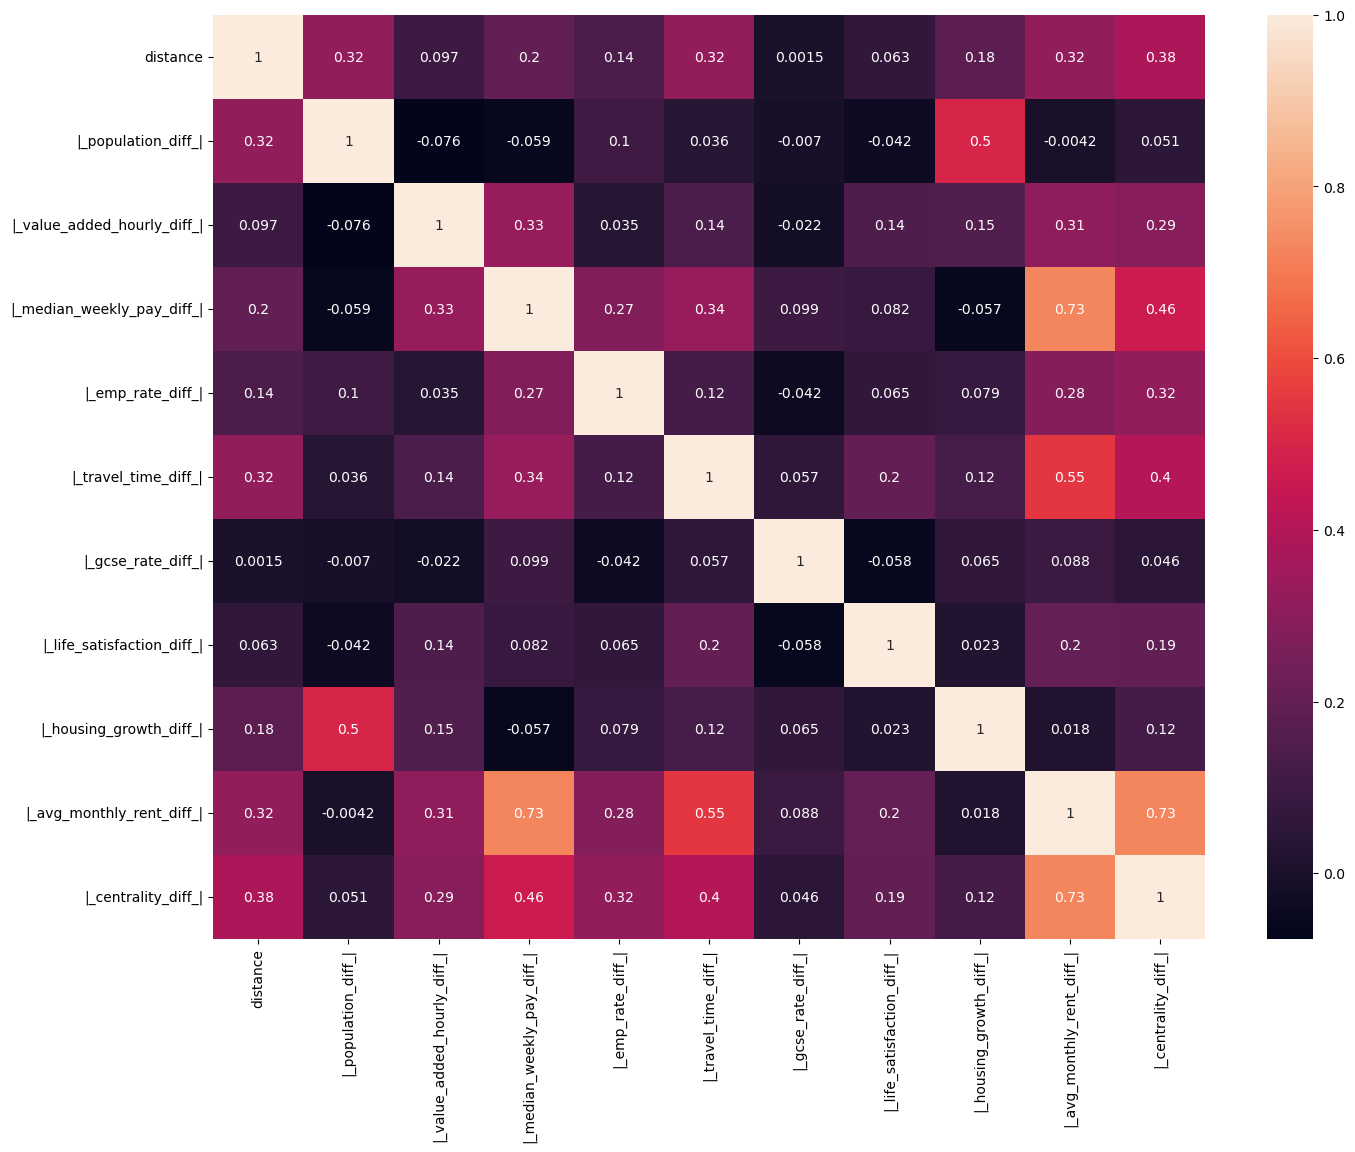
\includegraphics[keepaspectratio]{index_files/figure-pdf/cell-41-output-1.png}}

\begin{Shaded}
\begin{Highlighting}[]
\NormalTok{vif }\OperatorTok{=}\NormalTok{ pd.DataFrame()}
\NormalTok{vif[}\StringTok{\textquotesingle{}Variable\textquotesingle{}}\NormalTok{] }\OperatorTok{=}\NormalTok{ X.columns}
\NormalTok{vif[}\StringTok{\textquotesingle{}VIF\textquotesingle{}}\NormalTok{] }\OperatorTok{=}\NormalTok{ [variance\_inflation\_factor(X.values, i) }\ControlFlowTok{for}\NormalTok{ i }\KeywordTok{in} \BuiltInTok{range}\NormalTok{(X.shape[}\DecValTok{1}\NormalTok{])]}

\NormalTok{vif}
\end{Highlighting}
\end{Shaded}

\begin{longtable}[]{@{}lll@{}}
\toprule\noalign{}
& Variable & VIF \\
\midrule\noalign{}
\endhead
\bottomrule\noalign{}
\endlastfoot
0 & const & 1.000000 \\
1 & distance & 1.369576 \\
2 & \textbar\_population\_diff\_\textbar{} & 1.534792 \\
3 & \textbar\_value\_added\_hourly\_diff\_\textbar{} & 1.261580 \\
4 & \textbar\_median\_weekly\_pay\_diff\_\textbar{} & 2.389630 \\
5 & \textbar\_emp\_rate\_diff\_\textbar{} & 1.178689 \\
6 & \textbar\_travel\_time\_diff\_\textbar{} & 1.546928 \\
7 & \textbar\_gcse\_rate\_diff\_\textbar{} & 1.037265 \\
8 & \textbar\_life\_satisfaction\_diff\_\textbar{} & 1.085963 \\
9 & \textbar\_housing\_growth\_diff\_\textbar{} & 1.481976 \\
10 & \textbar\_avg\_monthly\_rent\_diff\_\textbar{} & 4.340401 \\
11 & \textbar\_centrality\_diff\_\textbar{} & 2.460915 \\
\end{longtable}

The correlation matrix shows limited collinearity between the variables,
with the greatest correlation between
\texttt{\textquotesingle{}avg\_monthly\_rent\_diff\textquotesingle{}}
and
\texttt{\textquotesingle{}median\_weekly\_pay\_diff\textquotesingle{}}
(0.73). This is not unexpected, as areas with higher rents will
generally require a higher wage rate to afford the rent.

The VIF analysis corroborates this limited collinearity, as all values
are below 10, a common concern threshold. All values are above 1, which
indicates some level of collinearity present, again with the greatest
values being
\texttt{\textquotesingle{}avg\_monthly\_rent\_diff\textquotesingle{}}
(4.3) and
\texttt{\textquotesingle{}median\_weekly\_pay\_diff\textquotesingle{}}
(2.4).

Multicollinearity violates the OLS assumptions and can lead to biased
coefficient estimates, so it is important to accommodate for this. The
OLS results show that
\texttt{\textquotesingle{}avg\_monthly\_rent\_diff\textquotesingle{}} is
more significant than
\texttt{\textquotesingle{}median\_weekly\_pay\_diff\textquotesingle{}},
has a larger coefficient, and is more precise, however, the VIF results
show it also has greater collinearity with other variables. To optimise
for the OLS assumptions, and to avoid the
\texttt{\textquotesingle{}avg\_monthly\_rent\_diff\textquotesingle{}}
soaking up explanatory power from correlated variables, I will drop it
from the model in future iterations. This is, again, a
researcher-driven, subjective decision.

\subsection{Refined Linear
Regression}\label{sec-refined-linear-regression}

Multiple paths can be taken to address the data's skewness (shown in
Figure~\ref{fig-histogram}). The most common is to use a log
transformation. However, the absolute difference variables include zero
values, which do not work with a log transformation. Therefore, a
Yeo-Johnson transformation is used, a generalisation of the log
transformation that can handle negative values (Yeo and Johnson, 2000).

\begin{Shaded}
\begin{Highlighting}[]
\NormalTok{columns\_OLSr }\OperatorTok{=}\NormalTok{ [col }\ControlFlowTok{for}\NormalTok{ col }\KeywordTok{in}\NormalTok{ commuteOLSr.columns }\ControlFlowTok{if}\NormalTok{ col }\KeywordTok{not} \KeywordTok{in}\NormalTok{ [}\StringTok{\textquotesingle{}journey\_score\textquotesingle{}}\NormalTok{, }\StringTok{\textquotesingle{}pairs\textquotesingle{}}\NormalTok{, }\StringTok{\textquotesingle{}route\_midpoint\_(geo)\textquotesingle{}}\NormalTok{]]}
\NormalTok{transformer }\OperatorTok{=}\NormalTok{ PowerTransformer(method}\OperatorTok{=}\StringTok{\textquotesingle{}yeo{-}johnson\textquotesingle{}}\NormalTok{, standardize}\OperatorTok{=}\VariableTok{True}\NormalTok{)}
\NormalTok{commuteOLSr[columns\_OLSr] }\OperatorTok{=}\NormalTok{ transformer.fit\_transform(commuteOLSr[columns\_OLSr])}
\end{Highlighting}
\end{Shaded}

And running a new OLS regression with the transformed data (with dropped
\texttt{\textquotesingle{}avg\_monthly\_rent\_diff\textquotesingle{}}):

\begin{Shaded}
\begin{Highlighting}[]
\NormalTok{y }\OperatorTok{=}\NormalTok{ commuteOLSr[}\StringTok{\textquotesingle{}journey\_score\textquotesingle{}}\NormalTok{]}
\NormalTok{X }\OperatorTok{=}\NormalTok{ commuteOLSr[[}\StringTok{\textquotesingle{}distance\textquotesingle{}}\NormalTok{, }\StringTok{\textquotesingle{}|\_population\_diff\_|\textquotesingle{}}\NormalTok{, }\StringTok{\textquotesingle{}|\_value\_added\_hourly\_diff\_|\textquotesingle{}}\NormalTok{,}
                \StringTok{\textquotesingle{}|\_median\_weekly\_pay\_diff\_|\textquotesingle{}}\NormalTok{, }\StringTok{\textquotesingle{}|\_emp\_rate\_diff\_|\textquotesingle{}}\NormalTok{,}
                 \StringTok{\textquotesingle{}|\_travel\_time\_diff\_|\textquotesingle{}}\NormalTok{, }\StringTok{\textquotesingle{}|\_gcse\_rate\_diff\_|\textquotesingle{}}\NormalTok{,}
                 \StringTok{\textquotesingle{}|\_life\_satisfaction\_diff\_|\textquotesingle{}}\NormalTok{, }\StringTok{\textquotesingle{}|\_housing\_growth\_diff\_|\textquotesingle{}}\NormalTok{,}
                 \StringTok{\textquotesingle{}|\_centrality\_diff\_|\textquotesingle{}}\NormalTok{]]}
\NormalTok{X }\OperatorTok{=}\NormalTok{ sm.add\_constant(X)}

\NormalTok{rlr\_model }\OperatorTok{=}\NormalTok{ sm.OLS(y, X).fit()}

\BuiltInTok{print}\NormalTok{(rlr\_model.summary())}
\end{Highlighting}
\end{Shaded}

\begin{verbatim}
                            OLS Regression Results                            
==============================================================================
Dep. Variable:          journey_score   R-squared:                       0.438
Model:                            OLS   Adj. R-squared:                  0.430
Method:                 Least Squares   F-statistic:                     51.99
Date:                Mon, 05 May 2025   Prob (F-statistic):           7.24e-77
Time:                        14:31:05   Log-Likelihood:                -164.77
No. Observations:                 677   AIC:                             351.5
Df Residuals:                     666   BIC:                             401.2
Df Model:                          10                                         
Covariance Type:            nonrobust                                         
===============================================================================================
                                  coef    std err          t      P>|t|      [0.025      0.975]
-----------------------------------------------------------------------------------------------
const                           0.3031      0.012     25.343      0.000       0.280       0.327
distance                       -0.2759      0.013    -21.054      0.000      -0.302      -0.250
|_population_diff_|             0.0593      0.013      4.449      0.000       0.033       0.086
|_value_added_hourly_diff_|    -0.0050      0.013     -0.387      0.699      -0.031       0.021
|_median_weekly_pay_diff_|     -0.0367      0.014     -2.649      0.008      -0.064      -0.009
|_emp_rate_diff_|               0.0188      0.013      1.494      0.136      -0.006       0.044
|_travel_time_diff_|            0.0180      0.014      1.294      0.196      -0.009       0.045
|_gcse_rate_diff_|             -0.0139      0.012     -1.148      0.252      -0.038       0.010
|_life_satisfaction_diff_|     -0.0079      0.012     -0.635      0.525      -0.032       0.016
|_housing_growth_diff_|         0.0373      0.013      2.806      0.005       0.011       0.063
|_centrality_diff_|            -0.0192      0.014     -1.390      0.165      -0.046       0.008
==============================================================================
Omnibus:                       60.620   Durbin-Watson:                   1.604
Prob(Omnibus):                  0.000   Jarque-Bera (JB):               75.204
Skew:                           0.764   Prob(JB):                     4.67e-17
Kurtosis:                       3.573   Cond. No.                         2.14
==============================================================================

Notes:
[1] Standard Errors assume that the covariance matrix of the errors is correctly specified.
\end{verbatim}

\subsubsection{Interpretation of the OLS
results}\label{sec-interpretation-ols-2}

General OLS considerations:

\begin{itemize}
\tightlist
\item
  R-squared = 0.438, indicates that c.43.8\% of the variation in
  \texttt{\textquotesingle{}journey\_score\textquotesingle{}} is
  explained by the linear combination of predictors, an improvement from
  the previous model (c.20.1\%)

  \begin{itemize}
  \tightlist
  \item
    This is helpful for inference, as it suggests that the model is
    better at explaining the variation in the data, and therefore the
    coefficients are more reliable
  \end{itemize}
\item
  F-statistic = 51.99 (p = c.0)

  \begin{itemize}
  \tightlist
  \item
    Given the p-value is effectively zero, the model is again
    statistically significant for explaining some aspects of the
    variation
  \end{itemize}
\end{itemize}

Key Variable:

\begin{itemize}
\tightlist
\item
  \texttt{\textquotesingle{}distance\textquotesingle{}}, is the most
  influential with the largest coefficient (0.2759), an even larger
  effect than the previous model (+62.7\%)

  \begin{itemize}
  \tightlist
  \item
    As a result of the transformation, we can no longer make an
    inference on the marginal impact of a unit change without
    back-transforming, which is a trade-off
  \item
    It is statistically significant (p \textless{} 0.001), and
    therefore, again we can be confident that this is a real effect
  \item
    The narrow confidence interval and large t-statistic implies a
    precisely estimated and statistically reliable effect
  \end{itemize}
\end{itemize}

Other variables:

\begin{itemize}
\tightlist
\item
  With the new specification,
  \texttt{\textquotesingle{}travel\_time\_diff\textquotesingle{}} is no
  longer significant at a 95\% confidence level
\item
  From the OLS summary, the significant variables ranked (by absolute
  size of coefficient) are as follows:
\end{itemize}

\begin{longtable}[]{@{}
  >{\raggedright\arraybackslash}p{(\linewidth - 10\tabcolsep) * \real{0.0190}}
  >{\raggedright\arraybackslash}p{(\linewidth - 10\tabcolsep) * \real{0.1709}}
  >{\raggedright\arraybackslash}p{(\linewidth - 10\tabcolsep) * \real{0.1076}}
  >{\raggedright\arraybackslash}p{(\linewidth - 10\tabcolsep) * \real{0.1456}}
  >{\raggedright\arraybackslash}p{(\linewidth - 10\tabcolsep) * \real{0.0570}}
  >{\raggedright\arraybackslash}p{(\linewidth - 10\tabcolsep) * \real{0.5000}}@{}}
\toprule\noalign{}
\begin{minipage}[b]{\linewidth}\raggedright
\#
\end{minipage} & \begin{minipage}[b]{\linewidth}\raggedright
Variable
\end{minipage} & \begin{minipage}[b]{\linewidth}\raggedright
Coefficient (β)
\end{minipage} & \begin{minipage}[b]{\linewidth}\raggedright
95\% CI
\end{minipage} & \begin{minipage}[b]{\linewidth}\raggedright
p-value
\end{minipage} & \begin{minipage}[b]{\linewidth}\raggedright
Relative to Simple OLS
\end{minipage} \\
\midrule\noalign{}
\endhead
\bottomrule\noalign{}
\endlastfoot
1 & \texttt{distance} & -0.2728 & {[}-0.302, -0.250{]} & 0.000 &
Stronger negative effect, still highly significant and precisely
estimated \\
2 & \texttt{population\_diff} & +0.0593 & {[}0.033, 0.086{]} & 0.000 &
Stronger positive effect, significant and generally precise \\
3 & \texttt{housing\_growth\_diff} & +0.0373 & {[}0.011, 0.063{]} &
0.005 & Weaker positive effect, significant (but not at 0.1\%) and
generally precise \\
4 & \texttt{median\_weekly\_pay\_diff} & -0.0367 & {[}-0.064, -0.009{]}
& 0.001 & Stronger negative effect, now significant \\
- & All others & - & CI include 0 & \textgreater0.05 & No statistical
significant 95\% confidence \\
\end{longtable}

The addition of
\texttt{\textquotesingle{}median\_weekly\_pay\_diff\textquotesingle{}}
suggests that the correlation with
\texttt{\textquotesingle{}avg\_monthly\_rent\_diff\textquotesingle{}}
may have impacted the inference of the previous model, whereas the
exclusion of
\texttt{\textquotesingle{}travel\_time\_diff\textquotesingle{}} may
reflect the change in distribution following the transformation.

Following this, permutation importance:

\begin{Shaded}
\begin{Highlighting}[]
\NormalTok{y\_pred }\OperatorTok{=}\NormalTok{ rlr\_model.predict(X)}
\NormalTok{baseline\_r2 }\OperatorTok{=}\NormalTok{ r2\_score(y, y\_pred)}

\NormalTok{feature\_importances }\OperatorTok{=}\NormalTok{ \{\}}

\ControlFlowTok{for}\NormalTok{ col }\KeywordTok{in}\NormalTok{ X.columns[}\DecValTok{1}\NormalTok{:]:}
\NormalTok{    np.random.seed(}\DecValTok{0}\NormalTok{) }\CommentTok{\# for reproducibility}
\NormalTok{    X\_permuted }\OperatorTok{=}\NormalTok{ X.copy()}
\NormalTok{    X\_permuted[col] }\OperatorTok{=}\NormalTok{ np.random.permutation(X\_permuted[col])}
\NormalTok{    y\_permuted\_pred }\OperatorTok{=}\NormalTok{ rlr\_model.predict(X\_permuted)}
\NormalTok{    permuted\_r2 }\OperatorTok{=}\NormalTok{ r2\_score(y, y\_permuted\_pred)}
\NormalTok{    feature\_importances[col] }\OperatorTok{=}\NormalTok{ baseline\_r2 }\OperatorTok{{-}}\NormalTok{ permuted\_r2}

\NormalTok{perm\_importance }\OperatorTok{=}\NormalTok{ pd.DataFrame(}\BuiltInTok{list}\NormalTok{(feature\_importances.items()), columns}\OperatorTok{=}\NormalTok{[}
                               \StringTok{\textquotesingle{}Variable\textquotesingle{}}\NormalTok{, }\StringTok{\textquotesingle{}Permutation Importance\textquotesingle{}}\NormalTok{])}
\NormalTok{perm\_importance }\OperatorTok{=}\NormalTok{ perm\_importance.sort\_values(}
\NormalTok{    by}\OperatorTok{=}\StringTok{\textquotesingle{}Permutation Importance\textquotesingle{}}\NormalTok{, ascending}\OperatorTok{=}\VariableTok{False}\NormalTok{)}

\NormalTok{perm\_importance.head(}\DecValTok{4}\NormalTok{) }\CommentTok{\# only need to show top 4 to compare}
\end{Highlighting}
\end{Shaded}

\begin{longtable}[]{@{}lll@{}}
\toprule\noalign{}
& Variable & Permutation Importance \\
\midrule\noalign{}
\endhead
\bottomrule\noalign{}
\endlastfoot
0 & distance & 0.871311 \\
1 & \textbar\_population\_diff\_\textbar{} & 0.038663 \\
3 & \textbar\_median\_weekly\_pay\_diff\_\textbar{} & 0.020285 \\
8 & \textbar\_housing\_growth\_diff\_\textbar{} & 0.017100 \\
\end{longtable}

The results corroborate the Refined OLS with the four most influential
variables and are again broadly consistent with the order.

Finally, with the dropped variable and transformed data, we can once
again check for multicollinearity:

\subsubsection{Multicollinearity}\label{sec-multicollinearity-ols-2}

\begin{Shaded}
\begin{Highlighting}[]
\NormalTok{commuteOLSrcm }\OperatorTok{=}\NormalTok{ commuteOLSr.drop(columns}\OperatorTok{=}\NormalTok{[}\StringTok{\textquotesingle{}pairs\textquotesingle{}}\NormalTok{, }\StringTok{\textquotesingle{}journey\_score\textquotesingle{}}\NormalTok{, }\StringTok{\textquotesingle{}route\_midpoint\_(geo)\textquotesingle{}}\NormalTok{])}

\NormalTok{plt.figure(figsize}\OperatorTok{=}\NormalTok{(}\DecValTok{16}\NormalTok{, }\DecValTok{12}\NormalTok{)) }
\NormalTok{sns.heatmap(commuteOLSrcm.corr(), annot}\OperatorTok{=}\VariableTok{True}\NormalTok{)}
\end{Highlighting}
\end{Shaded}

\pandocbounded{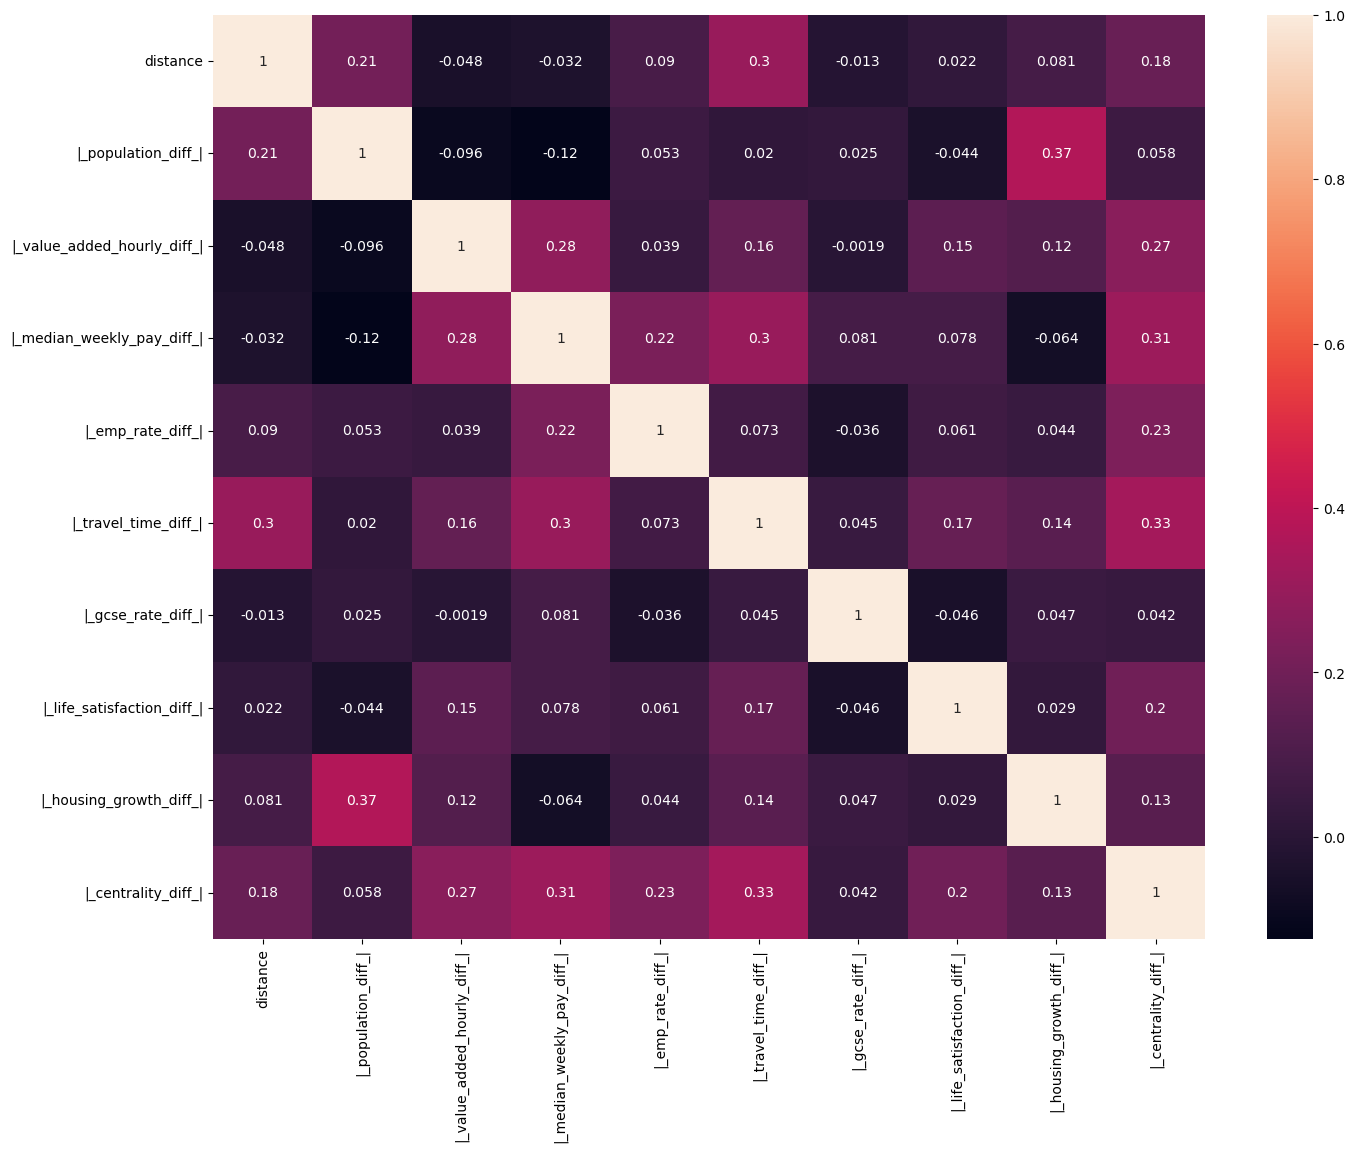
\includegraphics[keepaspectratio]{index_files/figure-pdf/cell-47-output-1.png}}

\begin{Shaded}
\begin{Highlighting}[]
\NormalTok{vif }\OperatorTok{=}\NormalTok{ pd.DataFrame()}
\NormalTok{vif[}\StringTok{\textquotesingle{}Variable\textquotesingle{}}\NormalTok{] }\OperatorTok{=}\NormalTok{ X.columns}
\NormalTok{vif[}\StringTok{\textquotesingle{}VIF\textquotesingle{}}\NormalTok{] }\OperatorTok{=}\NormalTok{ [variance\_inflation\_factor(X.values, i) }\ControlFlowTok{for}\NormalTok{ i }\KeywordTok{in} \BuiltInTok{range}\NormalTok{(X.shape[}\DecValTok{1}\NormalTok{])]}

\NormalTok{vif}
\end{Highlighting}
\end{Shaded}

\begin{longtable}[]{@{}lll@{}}
\toprule\noalign{}
& Variable & VIF \\
\midrule\noalign{}
\endhead
\bottomrule\noalign{}
\endlastfoot
0 & const & 1.000000 \\
1 & distance & 1.200264 \\
2 & \textbar\_population\_diff\_\textbar{} & 1.243007 \\
3 & \textbar\_value\_added\_hourly\_diff\_\textbar{} & 1.188374 \\
4 & \textbar\_median\_weekly\_pay\_diff\_\textbar{} & 1.338856 \\
5 & \textbar\_emp\_rate\_diff\_\textbar{} & 1.108864 \\
6 & \textbar\_travel\_time\_diff\_\textbar{} & 1.348697 \\
7 & \textbar\_gcse\_rate\_diff\_\textbar{} & 1.018920 \\
8 & \textbar\_life\_satisfaction\_diff\_\textbar{} & 1.072590 \\
9 & \textbar\_housing\_growth\_diff\_\textbar{} & 1.233093 \\
10 & \textbar\_centrality\_diff\_\textbar{} & 1.333514 \\
\end{longtable}

Where the concerns around multicollinearity are reduced.

\subsubsection{Discussion}\label{sec-discussion-ols-2}

Generally the results are similar to the previous OLS:

\begin{itemize}
\item
  The top three variables in the new results are all within the top five
  of the previous OLS

  \begin{itemize}
  \item
    The addition of
    \texttt{\textquotesingle{}median\_weekly\_pay\_diff\textquotesingle{}}
    is consistent with previous results due to its correlation with
    \texttt{\textquotesingle{}avg\_monthly\_rent\_diff\textquotesingle{}}
    which was dropped

    \begin{itemize}
    \tightlist
    \item
      Interetestingly the signs are different, suggesting as the
      differnce in median weekly pay increases, the
      \texttt{\textquotesingle{}journey\_score\textquotesingle{}}
      decreases
    \end{itemize}
  \end{itemize}
\item
  The order of influence/importance is the same across both the Simple
  and Refined OLS for the shared variables
\item
  \texttt{\textquotesingle{}distance\textquotesingle{}} is materially
  ahead of the other variables for both, and is the only variable with a
  coefficient above 0.1 in either model
\end{itemize}

With the transformation,
\texttt{\textquotesingle{}distance\textquotesingle{}} is an even more
important predictor of
\texttt{\textquotesingle{}journey\_score\textquotesingle{}}, with a
larger coefficient (0.2728, +62.7\% relative to simple OLS) and a more
precise estimate. As intuitive as this is, it still must be critically
challenged. This had been partially addressed by using absolute
differences in other variables so they are directionless too.

What remains unconsidered is the potential for spatial autocorrelation,
which is a key concern in geospatial data. A disproportionate amount of
data points near and within London is observed in the
Figure~\ref{fig-geo} produced in Appendix B: Section~\ref{sec-eda}.
Here, distances are shorter, and commuting flows more popular, which
could inflate the role of
\texttt{\textquotesingle{}distance\textquotesingle{}} while
underestimating the influence of other socio-economic structure
variables. In dense areas like London, shorter distances are still
popular, however this may not be because they are short, but due to
other factors, e.g.~high job density. In addition, socio-economic
factors are likely to be more similar nearby, therefore, OLS may not be
able to separate the two, instead attributing the high flows to distance
alone. Given the potential sampling bias with the overrepresentation of
structurally similar regions located near each other, these issues may
be magnified as those relationships, in turn, dominate the model.
Therefore, addressing some elements of spatial autocorrelation may be
necessary.

\subsection{Spatial Error Model (SEM)}\label{sec-sem}

I use spatial models (e.g., Spatial Error or Lag Models) where residuals
may be spatially autocorrelated, as otherwise, the OLS assumption of
independence of errors is violated, and inference restricted. Spatial
models can account for spatial structure within the residuals and,
therefore, if autocorrelation is present, are more reliable than a
standard OLS regression. Clustering in commuting flows relating to types
of roles has been discussed in the literature (Hincks et al., 2018), and
it is reasonable to assume that this may also be present in the data,
impacting other variables. Therefore, this will give me more confidence
in the inference I can draw to answer the research question.

\begin{tcolorbox}[enhanced jigsaw, colframe=quarto-callout-caution-color-frame, opacityback=0, breakable, toptitle=1mm, titlerule=0mm, coltitle=black, colback=white, bottomtitle=1mm, left=2mm, arc=.35mm, leftrule=.75mm, opacitybacktitle=0.6, bottomrule=.15mm, colbacktitle=quarto-callout-caution-color!10!white, title=\textcolor{quarto-callout-caution-color}{\faFire}\hspace{0.5em}{Further Information on Spatial Error Models (SEM)}, rightrule=.15mm, toprule=.15mm]

The form of the model is (Harris and Jarvis, 2011):

\[
y = \beta_0 + \beta_1 x_1 + \beta_2 x_2 + \cdots + \lambda \mathbf{W} \xi + \varepsilon
\]

Where:

\begin{itemize}
\item
  \(y\) is the dependent variable
\item
  \(x_1, x_2,...x_n\) are the independent variables
\item
  \(\beta_0\) is the intercept
\item
  \(\beta_1, \beta_2,...\beta_n\) are the coefficients
\item
  \(\lambda\) is the spatial autocorrelation coefficient
\item
  \(\mathbf{W}\) is the spatial weights matrix (i.e defines how
  observations are spatially connected)
\item
  \(\xi\) is the spatially correlated error term
\item
  \(\varepsilon\) is the error term for errors not spatially correlated
\end{itemize}

Key Assumptions Specific to SEM:

\begin{itemize}
\item
  Spatial autocorrelation in residuals: The error term shows a spatial
  relationship, captured by \(\lambda \mathbf{W} \xi\). This can be
  tested for using Moran's I
\item
  Correct specification of spatial weights: The matrix \(\mathbf{W}\)
  must should accurately reflect the true spatial structure
  (e.g.~distance-based vs kNN)
\item
  No omitted spatial structure: All spatial dependence is captured
  within the relevant error term
\end{itemize}

All other assumptions (e.g.~linearity, no perfect multicollinearity,
homoscedasticity) are the same as in an OLS regression

\end{tcolorbox}

The SEM is a generalisation of the OLS model, and therefore, the same
assumptions apply. The SEM also includes an additional assumption that
the error term is spatially autocorrelated, which is the key difference
between the two models.

I ran two spatial weight specification types (distance-based and
k-nearest neighbours (kNN)) at various thresholds to mimic sensitivity
analysis.

Distance-based weights define neighbours by the physical distance for a
given threshold, and kNN defines neighbours by the number of nearest
neighbours:

\begin{Shaded}
\begin{Highlighting}[]
\NormalTok{commuteSEM[}\StringTok{\textquotesingle{}residuals\textquotesingle{}}\NormalTok{] }\OperatorTok{=}\NormalTok{ rlr\_model.resid}

\NormalTok{d\_thresholds }\OperatorTok{=}\NormalTok{ [}\DecValTok{10000}\NormalTok{, }\DecValTok{20000}\NormalTok{, }\DecValTok{50000}\NormalTok{, }\DecValTok{100000}\NormalTok{, }\DecValTok{200000}\NormalTok{]  }\CommentTok{\# in m by default}
\NormalTok{k }\OperatorTok{=}\NormalTok{ [}\DecValTok{1}\NormalTok{, }\DecValTok{2}\NormalTok{, }\DecValTok{5}\NormalTok{, }\DecValTok{10}\NormalTok{, }\DecValTok{20}\NormalTok{]}
\NormalTok{results }\OperatorTok{=}\NormalTok{ \{}\StringTok{\textquotesingle{}Distance{-}based\textquotesingle{}}\NormalTok{: [], }\StringTok{\textquotesingle{}kNN\textquotesingle{}}\NormalTok{: []\}}

\NormalTok{warnings.filterwarnings(}
    \StringTok{\textquotesingle{}ignore\textquotesingle{}}\NormalTok{, message}\OperatorTok{=}\StringTok{"The weights matrix is not fully connected*"}\NormalTok{) }\CommentTok{\# get rid of error messags but can discuss}

\CommentTok{\# distance{-}based }
\ControlFlowTok{for}\NormalTok{ d }\KeywordTok{in}\NormalTok{ d\_thresholds:}
\NormalTok{    w }\OperatorTok{=}\NormalTok{ DistanceBand.from\_dataframe(}
\NormalTok{        commuteSEM, threshold}\OperatorTok{=}\NormalTok{d, silence\_warnings}\OperatorTok{=}\VariableTok{True}\NormalTok{)}
\NormalTok{    w.transform }\OperatorTok{=} \StringTok{\textquotesingle{}r\textquotesingle{}}
\NormalTok{    morani }\OperatorTok{=}\NormalTok{ Moran(commuteSEM[}\StringTok{\textquotesingle{}residuals\textquotesingle{}}\NormalTok{], w)}
\NormalTok{    results[}\StringTok{\textquotesingle{}Distance{-}based\textquotesingle{}}\NormalTok{].append((d }\OperatorTok{/} \DecValTok{1000}\NormalTok{, morani.I, morani.p\_sim)) }\CommentTok{\# switching to km}

\CommentTok{\# kNN}
\ControlFlowTok{for}\NormalTok{ k }\KeywordTok{in}\NormalTok{ k:}
\NormalTok{    w }\OperatorTok{=}\NormalTok{ KNN.from\_dataframe(commuteSEM, k}\OperatorTok{=}\NormalTok{k)}
\NormalTok{    w.transform }\OperatorTok{=} \StringTok{\textquotesingle{}r\textquotesingle{}}
\NormalTok{    morani }\OperatorTok{=}\NormalTok{ Moran(commuteSEM[}\StringTok{\textquotesingle{}residuals\textquotesingle{}}\NormalTok{], w)}
\NormalTok{    results[}\StringTok{\textquotesingle{}kNN\textquotesingle{}}\NormalTok{].append((k, morani.I, morani.p\_sim))}

\NormalTok{distance }\OperatorTok{=}\NormalTok{ pd.DataFrame(results[}\StringTok{\textquotesingle{}Distance{-}based\textquotesingle{}}\NormalTok{],}
\NormalTok{                       columns}\OperatorTok{=}\NormalTok{[}\StringTok{\textquotesingle{}Distance (km)\textquotesingle{}}\NormalTok{, }\StringTok{"Moran\textquotesingle{}s I"}\NormalTok{, }\StringTok{\textquotesingle{}p{-}value\textquotesingle{}}\NormalTok{])}
\NormalTok{knn }\OperatorTok{=}\NormalTok{ pd.DataFrame(results[}\StringTok{\textquotesingle{}kNN\textquotesingle{}}\NormalTok{], columns}\OperatorTok{=}\NormalTok{[}\StringTok{\textquotesingle{}k\textquotesingle{}}\NormalTok{, }\StringTok{"Moran\textquotesingle{}s I"}\NormalTok{, }\StringTok{\textquotesingle{}p{-}value\textquotesingle{}}\NormalTok{])}

\BuiltInTok{print}\NormalTok{(}\StringTok{"Moran\textquotesingle{}s I (distance{-}based):"}\NormalTok{)}
\BuiltInTok{print}\NormalTok{(distance)}
\BuiltInTok{print}\NormalTok{(}\StringTok{"}\CharTok{\textbackslash{}n}\StringTok{Moran\textquotesingle{}s I (kNN):"}\NormalTok{)}
\BuiltInTok{print}\NormalTok{(knn)}
\end{Highlighting}
\end{Shaded}

\begin{verbatim}
Moran's I (distance-based):
   Distance (km)  Moran's I  p-value
0           10.0   0.122814    0.001
1           20.0   0.118623    0.001
2           50.0   0.105237    0.001
3          100.0   0.072716    0.001
4          200.0   0.035270    0.001

Moran's I (kNN):
    k  Moran's I  p-value
0   1   0.065393    0.088
1   2   0.118213    0.001
2   5   0.135020    0.001
3  10   0.156095    0.001
4  20   0.143852    0.001
\end{verbatim}

I selected the kNN specification with 10 neighbours. At 0.156, the
Moran's I value suggests signficant spatial autocorrelation, and is the
highest value. The distance-based method adds neighbours in polynomial
(or near polynomial) form, leading to greater sensitivity in Moran I's
values. In addition, at most thresholds, not all points are connected
which would result in an exclusion of remote data points and therefore
bias the results. The kNN method is less sensitive to this, as it will
always include the same number of neighbours regardless of distance and
generally the kNN method is more interpretable, as it is easier to
understand the number of neighbours than the distance between them.

The selection between a Spatial Error Model (SEM) and e.g.~a Spatial Lag
Model (SLM) is based on the nature of the spatial autocorrelation
i.e.~SEM is when the spatial autocorrelation is in the residuals, and
SLM when in the dependent variable. To test this I use two Lagrange
Multiplier (LM) tests respectively:

\begin{Shaded}
\begin{Highlighting}[]
\NormalTok{w }\OperatorTok{=}\NormalTok{ KNN.from\_dataframe(commuteSEM, k}\OperatorTok{=}\DecValTok{10}\NormalTok{)}
\NormalTok{w.transform }\OperatorTok{=} \StringTok{\textquotesingle{}r\textquotesingle{}}
\NormalTok{ols\_model }\OperatorTok{=}\NormalTok{ OLS(y, X, w}\OperatorTok{=}\NormalTok{w, name\_y}\OperatorTok{=}\StringTok{\textquotesingle{}journey\_score\textquotesingle{}}\NormalTok{, name\_x}\OperatorTok{=}\NormalTok{X.columns.tolist(), name\_w}\OperatorTok{=}\StringTok{\textquotesingle{}kNN10\textquotesingle{}}\NormalTok{)}
\NormalTok{residuals }\OperatorTok{=}\NormalTok{ ols\_model.u }

\CommentTok{\# LM Error}
\NormalTok{slm\_res }\OperatorTok{=}\NormalTok{ lag\_spatial(w, residuals)}
\NormalTok{n }\OperatorTok{=} \BuiltInTok{len}\NormalTok{(y)}
\NormalTok{e }\OperatorTok{=}\NormalTok{ residuals}
\NormalTok{e\_lag }\OperatorTok{=}\NormalTok{ slm\_res}
\NormalTok{sse }\OperatorTok{=}\NormalTok{ np.}\BuiltInTok{sum}\NormalTok{(e}\OperatorTok{**}\DecValTok{2}\NormalTok{)}
\NormalTok{sse\_lag }\OperatorTok{=}\NormalTok{ np.}\BuiltInTok{sum}\NormalTok{(e }\OperatorTok{*}\NormalTok{ e\_lag)}
\NormalTok{lm\_error }\OperatorTok{=}\NormalTok{ (n }\OperatorTok{*}\NormalTok{ (sse\_lag}\OperatorTok{**}\DecValTok{2}\NormalTok{)) }\OperatorTok{/}\NormalTok{ (sse}\OperatorTok{**}\DecValTok{2}\NormalTok{)}
\NormalTok{lm\_error\_p }\OperatorTok{=} \DecValTok{1} \OperatorTok{{-}}\NormalTok{ stats.chi2.cdf(lm\_error, df}\OperatorTok{=}\DecValTok{1}\NormalTok{)}

\CommentTok{\# LM lag}
\NormalTok{y\_lag }\OperatorTok{=}\NormalTok{ lag\_spatial(w, y)}
\NormalTok{lm\_lag }\OperatorTok{=}\NormalTok{ (n }\OperatorTok{*}\NormalTok{ (np.}\BuiltInTok{sum}\NormalTok{(y\_lag }\OperatorTok{*}\NormalTok{ e)}\OperatorTok{**}\DecValTok{2}\NormalTok{)) }\OperatorTok{/}\NormalTok{ (sse }\OperatorTok{*}\NormalTok{ np.}\BuiltInTok{sum}\NormalTok{(y\_lag}\OperatorTok{**}\DecValTok{2}\NormalTok{))}
\NormalTok{lm\_lag\_p }\OperatorTok{=} \DecValTok{1} \OperatorTok{{-}}\NormalTok{ stats.chi2.cdf(lm\_lag, df}\OperatorTok{=}\DecValTok{1}\NormalTok{)}

\BuiltInTok{print}\NormalTok{(}\SpecialStringTok{f"LM Error test: }\SpecialCharTok{\{}\NormalTok{lm\_error}\SpecialCharTok{:.3f\}}\SpecialStringTok{, p{-}value: }\SpecialCharTok{\{}\NormalTok{lm\_error\_p}\SpecialCharTok{:.3f\}}\SpecialStringTok{"}\NormalTok{)}
\BuiltInTok{print}\NormalTok{(}\SpecialStringTok{f"LM Lag test: }\SpecialCharTok{\{}\NormalTok{lm\_lag}\SpecialCharTok{:.3f\}}\SpecialStringTok{, p{-}value: }\SpecialCharTok{\{}\NormalTok{lm\_lag\_p}\SpecialCharTok{:.3f\}}\SpecialStringTok{"}\NormalTok{)}
\end{Highlighting}
\end{Shaded}

\begin{verbatim}
LM Error test: 16.496, p-value: 0.000
LM Lag test: 0.000, p-value: 1.000
\end{verbatim}

The tests imply that spatial autocorrelation exists in the residuals but
not dependent variables, therefore a SEM is appropriate:

\begin{Shaded}
\begin{Highlighting}[]
\NormalTok{sem\_model }\OperatorTok{=}\NormalTok{ GM\_Error\_Het(y, X, w}\OperatorTok{=}\NormalTok{w, name\_ds}\OperatorTok{=}\StringTok{\textquotesingle{}commuteOLS\textquotesingle{}}\NormalTok{ , name\_w}\OperatorTok{=}\StringTok{"kNN, k=10"}\NormalTok{, hard\_bound}\OperatorTok{=}\VariableTok{True}\NormalTok{) }\CommentTok{\# SEM with heteroskedasticity}

\BuiltInTok{print}\NormalTok{(sem\_model.summary)}
\end{Highlighting}
\end{Shaded}

\begin{verbatim}
REGRESSION RESULTS
------------------

SUMMARY OF OUTPUT: GM SPATIALLY WEIGHTED LEAST SQUARES (HET)
------------------------------------------------------------
Data set            :  commuteOLS
Weights matrix      :   kNN, k=10
Dependent Variable  :journey_score                Number of Observations:         677
Mean dependent var  :      0.3031                Number of Variables   :          11
S.D. dependent var  :      0.4122                Degrees of Freedom    :         666
Pseudo R-squared    :      0.4137
N. of iterations    :           1                Step1c computed       :          No

------------------------------------------------------------------------------------
            Variable     Coefficient       Std.Error     z-Statistic     Probability
------------------------------------------------------------------------------------
            CONSTANT         0.31282         0.03323         9.41436         0.00000
            distance        -0.34893         0.01441       -24.20732         0.00000
 |_population_diff_|         0.03319         0.01295         2.56337         0.01037
|_value_added_hourly_diff_|        -0.00456         0.01158        -0.39342         0.69401
|_median_weekly_pay_diff_|        -0.01664         0.01283        -1.29742         0.19449
   |_emp_rate_diff_|         0.01863         0.01113         1.67371         0.09419
|_travel_time_diff_|         0.01954         0.01451         1.34692         0.17801
  |_gcse_rate_diff_|        -0.01647         0.01027        -1.60488         0.10852
|_life_satisfaction_diff_|         0.00155         0.01157         0.13438         0.89310
|_housing_growth_diff_|         0.03430         0.01250         2.74306         0.00609
 |_centrality_diff_|         0.02457         0.01331         1.84668         0.06479
              lambda         0.68295         0.03580        19.07529         0.00000
------------------------------------------------------------------------------------
Warning: Variable(s) ['const'] removed for being constant.
================================ END OF REPORT =====================================
\end{verbatim}

\subsubsection{Interpretation of the SEM
results}\label{sec-interpretation-sem}

General SEM considerations:

\begin{itemize}
\tightlist
\item
  (Pseudo) R-squared = 0.4137

  \begin{itemize}
  \tightlist
  \item
    This metric is not directly comparable to R-squared, but shows a
    goodness of fit relative to a model with no variables
  \item
    At 0.4137, this is a reasonable fit, explaining a fair amount of
    variation
  \end{itemize}
\end{itemize}

Key Variable:

\begin{itemize}
\tightlist
\item
  \texttt{\textquotesingle{}distance\textquotesingle{}}, is again the
  most influential with the largest coefficient (0.34893), continuing to
  dominate in terms of importance even after the consideration of
  spatial autcorrelation

  \begin{itemize}
  \tightlist
  \item
    It is statistically significant still (p \textless{} 0.001)
  \end{itemize}
\end{itemize}

Other variables:

\begin{itemize}
\tightlist
\item
  With the new model specification,
  \texttt{\textquotesingle{}median\_weekly\_pay\_diff\textquotesingle{}}
  is no longer significant at any confidence level
\item
  From the OLS summary, the significant variables ranked (by absolute
  size of coefficient) are as follows:
\end{itemize}

\begin{longtable}[]{@{}
  >{\raggedright\arraybackslash}p{(\linewidth - 8\tabcolsep) * \real{0.0224}}
  >{\raggedright\arraybackslash}p{(\linewidth - 8\tabcolsep) * \real{0.1791}}
  >{\raggedright\arraybackslash}p{(\linewidth - 8\tabcolsep) * \real{0.1269}}
  >{\raggedright\arraybackslash}p{(\linewidth - 8\tabcolsep) * \real{0.0672}}
  >{\raggedright\arraybackslash}p{(\linewidth - 8\tabcolsep) * \real{0.6045}}@{}}
\toprule\noalign{}
\begin{minipage}[b]{\linewidth}\raggedright
\#
\end{minipage} & \begin{minipage}[b]{\linewidth}\raggedright
Variable
\end{minipage} & \begin{minipage}[b]{\linewidth}\raggedright
Coefficient (β)
\end{minipage} & \begin{minipage}[b]{\linewidth}\raggedright
p-value
\end{minipage} & \begin{minipage}[b]{\linewidth}\raggedright
Interpretation vs Refined OLS
\end{minipage} \\
\midrule\noalign{}
\endhead
\bottomrule\noalign{}
\endlastfoot
1 & \texttt{distance} & -0.3489 & 0.000 & Stronger negative effect \\
2 & \texttt{population\_diff} & +0.0332 & 0.000 & Weaker positive
effect \\
3 & \texttt{housing\_growth\_diff} & +0.0343 & 0.006 & Weaker positive
effect \\
- & All others & - & \textgreater0.05 & Not statistically significant at
95\% confidence level \\
\end{longtable}

The hypothesis that spatial autocorrelation prevented the OLS from
seperating the impact of each vraiable driving the relationship was
correct. However the direction for
\texttt{\textquotesingle{}distance\textquotesingle{}} was wrong, in
actuality the other variables were soaking up the explanatory power of
\texttt{\textquotesingle{}distance\textquotesingle{}}, instead of the
other way around. Therefore, the SEM actually suggests that
\texttt{\textquotesingle{}distance\textquotesingle{}} is even more
important than the OLS.

The exclusion of
\texttt{\textquotesingle{}median\_weekly\_pay\_diff\textquotesingle{}}
is interesting, as it was significant in the OLS, but with a
counterintuitive negative relationship between difference and flow
popularity. This may have been due to spatial autocorrelation, proving
further evidence that the SEM adds insight to the inference task.

This is about as deep as I can go with linear regression, and even then,
it is not clear whether the SEM/OLS are robust enough, in terms of
satisfying key assumptions, to draw an inference with confidence.

This can be seen when assessing the residuals of the SEM:

\begin{Shaded}
\begin{Highlighting}[]
\NormalTok{sns.set\_theme(style}\OperatorTok{=}\StringTok{\textquotesingle{}darkgrid\textquotesingle{}}\NormalTok{)}
\NormalTok{palette }\OperatorTok{=}\NormalTok{ [}\StringTok{\textquotesingle{}\#69b3a2\textquotesingle{}}\NormalTok{]}

\NormalTok{plt.figure(figsize}\OperatorTok{=}\NormalTok{(}\DecValTok{8}\NormalTok{, }\DecValTok{6}\NormalTok{))}
\NormalTok{sns.scatterplot(x}\OperatorTok{=}\NormalTok{sem\_model.predy.flatten(),}
\NormalTok{                y}\OperatorTok{=}\NormalTok{sem\_model.u.flatten(), color}\OperatorTok{=}\NormalTok{palette[}\DecValTok{0}\NormalTok{])}
\NormalTok{plt.axhline(}\DecValTok{0}\NormalTok{, color}\OperatorTok{=}\StringTok{\textquotesingle{}red\textquotesingle{}}\NormalTok{, linestyle}\OperatorTok{=}\StringTok{\textquotesingle{}{-}{-}\textquotesingle{}}\NormalTok{)}
\NormalTok{plt.xlabel(}\StringTok{\textquotesingle{}Fitted values\textquotesingle{}}\NormalTok{)}
\NormalTok{plt.ylabel(}\StringTok{\textquotesingle{}Residuals\textquotesingle{}}\NormalTok{)}
\NormalTok{plt.title(}\StringTok{\textquotesingle{}Residuals vs Fitted\textquotesingle{}}\NormalTok{)}
\NormalTok{plt.tight\_layout()}
\NormalTok{plt.show()}
\end{Highlighting}
\end{Shaded}

\begin{figure}[H]

\centering{

\pandocbounded{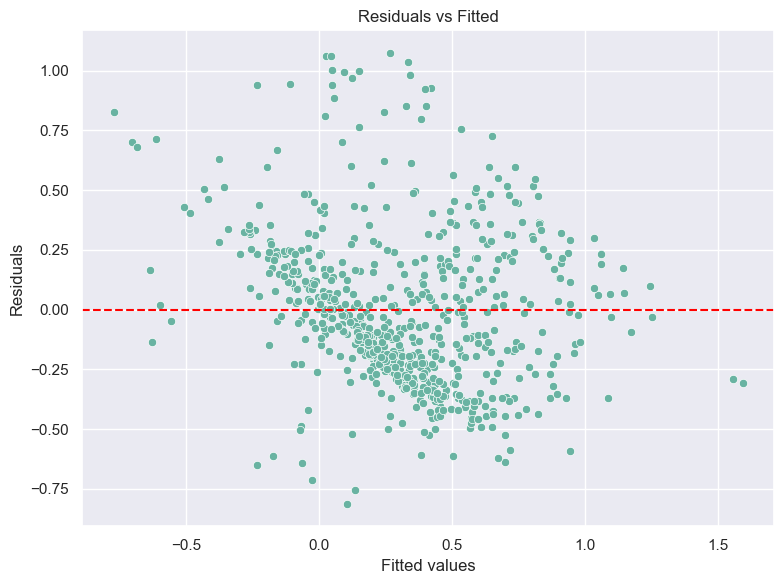
\includegraphics[keepaspectratio]{index_files/figure-pdf/fig-residuals-output-1.png}}

}

\caption{\label{fig-residuals}Scatterplot of residuals vs fitted values}

\end{figure}%

Here, we can see that despite best efforts, the variance of residuals
changes with fitted values, i.e.~heteroscedasticity persists.

\section{Random Forest}\label{sec-random-forest}

Given that the assumptions of linear regression may not be fully
satisfied in this context, I decide to use a Random Forest model which
may be more appropriate.

Random Forests are more robust for inference as they do not rely on
satisfying assumptions like linearity, homoscedasticity or independence
of residuals. They handle outliers, multicollinearity, and non-linear
relationships well, all of which may be relevant in this case.

The trade-off is that they do not provide effect sizes or directions
when assessing feature importance directly, however in combination with
the results of the regression models, they can provide a more complete
picture of the relationships between variables.

This is shown below, using the original dataset (i.e.~not standardised
or transformed):

\begin{Shaded}
\begin{Highlighting}[]
\NormalTok{y\_rf }\OperatorTok{=}\NormalTok{ commute[}\StringTok{\textquotesingle{}journey\_score\textquotesingle{}}\NormalTok{]}
\NormalTok{X\_rf }\OperatorTok{=}\NormalTok{ commute[[}\StringTok{\textquotesingle{}distance\textquotesingle{}}\NormalTok{, }\StringTok{\textquotesingle{}|\_population\_diff\_|\textquotesingle{}}\NormalTok{, }\StringTok{\textquotesingle{}|\_value\_added\_hourly\_diff\_|\textquotesingle{}}\NormalTok{,}
                \StringTok{\textquotesingle{}|\_median\_weekly\_pay\_diff\_|\textquotesingle{}}\NormalTok{, }\StringTok{\textquotesingle{}|\_emp\_rate\_diff\_|\textquotesingle{}}\NormalTok{,}
                 \StringTok{\textquotesingle{}|\_travel\_time\_diff\_|\textquotesingle{}}\NormalTok{, }\StringTok{\textquotesingle{}|\_gcse\_rate\_diff\_|\textquotesingle{}}\NormalTok{,}
                 \StringTok{\textquotesingle{}|\_life\_satisfaction\_diff\_|\textquotesingle{}}\NormalTok{, }\StringTok{\textquotesingle{}|\_housing\_growth\_diff\_|\textquotesingle{}}\NormalTok{,}
                 \StringTok{\textquotesingle{}|\_centrality\_diff\_|\textquotesingle{}}\NormalTok{]]}

\NormalTok{(X\_train,}
\NormalTok{ X\_test,}
\NormalTok{ y\_train,}
\NormalTok{ y\_test) }\OperatorTok{=}\NormalTok{ skm.train\_test\_split(X\_rf,}
\NormalTok{                                y\_rf,}
\NormalTok{                                test\_size}\OperatorTok{=}\FloatTok{0.2}\NormalTok{,}
\NormalTok{                                random\_state}\OperatorTok{=}\DecValTok{0}\NormalTok{)}

\NormalTok{commuteRF }\OperatorTok{=}\NormalTok{ RF(max\_features}\OperatorTok{=}\StringTok{\textquotesingle{}sqrt\textquotesingle{}}\NormalTok{,}
\NormalTok{               random\_state}\OperatorTok{=}\DecValTok{0}\NormalTok{).fit(X\_train, y\_train)}
\NormalTok{y\_hat\_RF }\OperatorTok{=}\NormalTok{ commuteRF.predict(X\_test)}
\NormalTok{mse }\OperatorTok{=}\NormalTok{ np.mean((y\_test }\OperatorTok{{-}}\NormalTok{ y\_hat\_RF)}\OperatorTok{**}\DecValTok{2}\NormalTok{)}
\NormalTok{r2 }\OperatorTok{=}\NormalTok{ r2\_score(y\_test, y\_hat\_RF)}

\BuiltInTok{print}\NormalTok{(}\SpecialStringTok{f"Mean Squared Error: }\SpecialCharTok{\{}\NormalTok{mse}\SpecialCharTok{.}\BuiltInTok{round}\NormalTok{(}\DecValTok{3}\NormalTok{)}\SpecialCharTok{\}}\SpecialStringTok{"}\NormalTok{)}
\BuiltInTok{print}\NormalTok{(}\SpecialStringTok{f"R{-}squared: }\SpecialCharTok{\{}\NormalTok{r2}\SpecialCharTok{.}\BuiltInTok{round}\NormalTok{(}\DecValTok{3}\NormalTok{)}\SpecialCharTok{\}}\SpecialStringTok{"}\NormalTok{)}
\end{Highlighting}
\end{Shaded}

\begin{verbatim}
Mean Squared Error: 0.084
R-squared: 0.485
\end{verbatim}

The R-squared of the Random Forest model is 0.485, which is a marginal
improvement on the linear regression models, implying that the random
forest is able to better capture the relationships between the variables

Rather than coefficients, the Random Forest model has a feature
importance metric, which is a measure of how much each variable
contributes to the model's predictions:

\begin{Shaded}
\begin{Highlighting}[]
\NormalTok{rif\_feature\_importance }\OperatorTok{=}\NormalTok{ pd.Series(commuteRF.feature\_importances\_, index}\OperatorTok{=}\NormalTok{X\_train.columns).sort\_values(ascending}\OperatorTok{=}\VariableTok{False}\NormalTok{)}
\NormalTok{rif\_feature\_importance}
\end{Highlighting}
\end{Shaded}

\begin{verbatim}
distance                       0.416896
|_population_diff_|            0.088291
|_housing_growth_diff_|        0.074278
|_travel_time_diff_|           0.073151
|_median_weekly_pay_diff_|     0.068869
|_centrality_diff_|            0.065763
|_value_added_hourly_diff_|    0.058756
|_gcse_rate_diff_|             0.054705
|_emp_rate_diff_|              0.051680
|_life_satisfaction_diff_|     0.047610
dtype: float64
\end{verbatim}

Here, we can see that the most important variable is
\texttt{\textquotesingle{}distance\textquotesingle{}} (0.4169), which is
consistent with the OLS and SEM results. The other variables again
include \texttt{\textquotesingle{}population\_diff\textquotesingle{}}
(0.0883) and
\texttt{\textquotesingle{}housing\_growth\_diff\textquotesingle{}}
(0.0743), consistent with the OLS and SEM results. However,
\texttt{\textquotesingle{}travel\_time\_diff\textquotesingle{}} (0.0732)
is now also included, and
\texttt{\textquotesingle{}median\_weekly\_pay\_diff\textquotesingle{}}
(0.0689) is not materially more important than the added
\texttt{\textquotesingle{}centrality\textquotesingle{}} variable
(0.0658).

As discussed, Random Forest models are non-parametric, and hence, there
is no additional information on concepts such as statistical
significance, effect size, or direction of the relationship, in the
scope of this method. Therefore, this is the extent of the inference.

And finally, permutation importance:

\begin{Shaded}
\begin{Highlighting}[]
\NormalTok{result }\OperatorTok{=}\NormalTok{ permutation\_importance(commuteRF, X\_test, y\_test,}
\NormalTok{                                 n\_repeats}\OperatorTok{=}\DecValTok{5}\NormalTok{,}
\NormalTok{                                 random\_state}\OperatorTok{=}\DecValTok{0}\NormalTok{)}

\NormalTok{rif\_perm\_importance }\OperatorTok{=}\NormalTok{ pd.Series(result.importances\_mean, index}\OperatorTok{=}\NormalTok{X\_test.columns).sort\_values(ascending}\OperatorTok{=}\VariableTok{False}\NormalTok{)}
\NormalTok{rif\_perm\_importance}
\end{Highlighting}
\end{Shaded}

\begin{verbatim}
distance                       0.680163
|_population_diff_|            0.156520
|_centrality_diff_|            0.038961
|_median_weekly_pay_diff_|     0.019008
|_emp_rate_diff_|              0.015234
|_travel_time_diff_|           0.012933
|_housing_growth_diff_|        0.011483
|_gcse_rate_diff_|             0.010611
|_life_satisfaction_diff_|    -0.000230
|_value_added_hourly_diff_|   -0.000486
dtype: float64
\end{verbatim}

The results are broadly consistent again, but
\texttt{\textquotesingle{}centrality\textquotesingle{}} is more
important than other metrics for the first time. Again, it is important
to note that there is an element of randomness in the results, and
therefore, they must be interpreted with caution.

\section{Conclusion}\label{sec-conclusion}

My research question asked:

``Which structural socioeconomic factors between regions most influence
the relative popularity of commuting routes?''

I employed three models to address this question: OLS, SEM, and Random
Forest. I used linear regressions as my primary method of analysis as
the models tend to have the most inferential power, providing insight
into importance, direction and effect size. However, the assumptions of
linear regression may not be fully satisfied in this context, and
therefore, I also employed a Random Forest model, which is more robust
to violations of the assumptions. Other models were not used, as
generally there is a trade-off between complexity and interpretability.

They key metrics used for inference were the coefficients of the OLS and
SEM models, and the feature importance of the Random Forest model. I
also used permutation importance across all, as it is a consistent
metric across models, however due to the random elements, the confidence
in their reults is lower. Other potential metrics such as Shapley
values, were briefly mentioned, but not employed for simplicity of the
task.

Results were generally consistent across the models. With high
confidence, I can say that
\texttt{\textquotesingle{}distance\textquotesingle{}} is the most
important structural variable that determines the relative popularity of
commuting routes, and this is consistent with the literature on the
subject (So et al., 2001). This was verified across all model types and
specifications, and in each case,
\texttt{\textquotesingle{}distance\textquotesingle{}} was materially
more important than the next best variable. In all regression models,
the coefficient of \texttt{\textquotesingle{}distance\textquotesingle{}}
was negative, indicating that as distance increases, the popularity of
the route decreases, and the results were statistically significant at
all confidence levels. However, the literature (So et al., 2001) also
focuses heavily on commuting time, which is not included in this
analysis and is likely to be heavily correlated with distance. This is a
key limitation of the analysis, as it is not possible to separate
variables like \texttt{\textquotesingle{}distance\textquotesingle{}}
from related factors, and therefore inference is limited abnd/or biased
by researcher design.

\texttt{\textquotesingle{}population\_diff\textquotesingle{}} was
consistently the second most important variable across models (excluding
the simple, pre-transformation OLS), and was statistically significant
in all OLS and SEM models. These models showed that the larger the
difference in the population, the higher the commuting flow's relative
popularity. This may reflect that larger populations by definiton have
more people who can commute, leading to a higher commuting flow. It also
may act as a proxy for other factors such as urban/rural splits, job
density and many other socioeconomic factors.

Other consistently important variables included
\texttt{\textquotesingle{}housing\_growth\_diff\textquotesingle{}} and
\texttt{\textquotesingle{}median\_weekly\_pay\_diff\textquotesingle{}},
where again, the greater the difference, the higher the relative
popularity of the commuting flow. Importance rankings and significance
varied across models, adding uncertainty to their interpretation. The
former could be a lagging indicator of demand and, therefore, may be a
proxy for other factors. The latter may reflect the economic trade-off
associated with commuting.

Other variables did not consistently provide explanatory power for the
relationship with commuting popularity, so I cannot draw any conclusions
about their importance.

\subsection*{References}\label{references}
\addcontentsline{toc}{subsection}{References}

\renewcommand{\bibsection}{}
\bibliography{references.bib}

\begin{center}\rule{0.5\linewidth}{0.5pt}\end{center}

\section{Appendices}\label{sec-appendices}

\subsection{Appendix A: Setup}\label{sec-setup}

\subsubsection{Environment}\label{sec-environment}

This notebook was written in Python 3.9.18. The environment can be
retrieved from the \href{https://github.com/2601547/commute}{Github
project repo}.

\subsubsection{Packages}\label{sec-packages}

\begin{Shaded}
\begin{Highlighting}[]
\ImportTok{import}\NormalTok{ os}
\ImportTok{import}\NormalTok{ random}
\ImportTok{import}\NormalTok{ warnings}

\ImportTok{import}\NormalTok{ contextily }\ImportTok{as}\NormalTok{ ctx}
\ImportTok{import}\NormalTok{ geopandas }\ImportTok{as}\NormalTok{ gpd}
\ImportTok{import}\NormalTok{ matplotlib.pyplot }\ImportTok{as}\NormalTok{ plt}
\ImportTok{import}\NormalTok{ networkx }\ImportTok{as}\NormalTok{ nx}
\ImportTok{import}\NormalTok{ numpy }\ImportTok{as}\NormalTok{ np}
\ImportTok{import}\NormalTok{ pandas }\ImportTok{as}\NormalTok{ pd}
\ImportTok{import}\NormalTok{ requests}
\ImportTok{import}\NormalTok{ seaborn }\ImportTok{as}\NormalTok{ sns}
\ImportTok{import}\NormalTok{ sklearn.model\_selection }\ImportTok{as}\NormalTok{ skm}
\ImportTok{import}\NormalTok{ statsmodels.api }\ImportTok{as}\NormalTok{ sm}

\ImportTok{from}\NormalTok{ esda.moran }\ImportTok{import}\NormalTok{ Moran}
\ImportTok{from}\NormalTok{ libpysal.weights }\ImportTok{import}\NormalTok{ DistanceBand, KNN, lag\_spatial}
\ImportTok{from}\NormalTok{ scipy }\ImportTok{import}\NormalTok{ stats}
\ImportTok{from}\NormalTok{ scipy.stats }\ImportTok{import}\NormalTok{ skew}
\ImportTok{from}\NormalTok{ sklearn.ensemble }\ImportTok{import}\NormalTok{ RandomForestRegressor }\ImportTok{as}\NormalTok{ RF}
\ImportTok{from}\NormalTok{ sklearn.inspection }\ImportTok{import}\NormalTok{ permutation\_importance}
\ImportTok{from}\NormalTok{ sklearn.metrics }\ImportTok{import}\NormalTok{ r2\_score}
\ImportTok{from}\NormalTok{ sklearn.preprocessing }\ImportTok{import}\NormalTok{ PowerTransformer, StandardScaler}
\ImportTok{from}\NormalTok{ spreg }\ImportTok{import}\NormalTok{ GM\_Error\_Het, OLS}
\ImportTok{from}\NormalTok{ statsmodels.stats.outliers\_influence }\ImportTok{import}\NormalTok{ variance\_inflation\_factor}
\end{Highlighting}
\end{Shaded}

\subsection{Appendix B: Exploratory Data Analysis}\label{sec-eda}

\begin{tcolorbox}[enhanced jigsaw, colframe=quarto-callout-tip-color-frame, opacityback=0, breakable, toptitle=1mm, titlerule=0mm, coltitle=black, colback=white, bottomtitle=1mm, left=2mm, arc=.35mm, leftrule=.75mm, opacitybacktitle=0.6, bottomrule=.15mm, colbacktitle=quarto-callout-tip-color!10!white, title=\textcolor{quarto-callout-tip-color}{\faLightbulb}\hspace{0.5em}{Section Summary}, rightrule=.15mm, toprule=.15mm]

\begin{itemize}
\item
  Cleaned the dataset by:

  \begin{itemize}
  \tightlist
  \item
    Dropping routes missing values (``City of London'' and ``Isles of
    Scilly'')
  \end{itemize}
\item
  Add geographic information, including coordinates, using
  \texttt{geopandas}

  \begin{itemize}
  \tightlist
  \item
    Identified potential spatial autocorrelation
  \end{itemize}
\item
  Identified daily variation in
  \texttt{\textquotesingle{}journey\_score\textquotesingle{}} for the
  same routes over time
\end{itemize}

\end{tcolorbox}

The following section addresses exploration of the provided dataset,
focusing on:

\begin{itemize}
\tightlist
\item
  Understanding the data
\item
  Ensuring the data is clean and usable
\item
  Visualising the data to understand the context and distribution
\end{itemize}

The LAcommute.csv file is loaded into a pandas dataframe and displayed:

\begin{Shaded}
\begin{Highlighting}[]
\CommentTok{\# relative file paths are used here as to not leak my name, although absolute paths may be better for reproducibility}
\NormalTok{base\_data\_dir }\OperatorTok{=}\NormalTok{ os.path.abspath(}\StringTok{\textquotesingle{}../../1. Data/LAcommute\textquotesingle{}}\NormalTok{)}
\NormalTok{LAcommute }\OperatorTok{=}\NormalTok{ pd.read\_csv(}
\NormalTok{    os.path.join(base\_data\_dir, }\StringTok{"LAcommute.csv"}\NormalTok{), index\_col}\OperatorTok{=}\DecValTok{0}\NormalTok{)}
\NormalTok{LAcommute}
\end{Highlighting}
\end{Shaded}

\begin{longtable}[]{@{}llllllllllllllllllllll@{}}
\toprule\noalign{}
& date & area\_name\_origin & area\_code\_origin & area\_name\_dest &
area\_code\_dest & journey\_score & journey\_count\_decile & distance &
population\_origin & population\_dest & ... & gcse\_rate\_origin &
life\_satisfaction\_origin & housing\_growth\_origin &
value\_added\_hourly\_dest & median\_weekly\_pay\_dest & emp\_rate\_dest
& travel\_time\_dest & gcse\_rate\_dest & life\_satisfaction\_dest &
housing\_growth\_dest \\
\midrule\noalign{}
\endhead
\bottomrule\noalign{}
\endlastfoot
0 & 2019-01-01 & Hartlepool & E06000001 & Hartlepool & E06000001 &
1.4414 & 9 & 0.000000 & 92401 & 92401 & ... & 67.6 & 7.33 & 161 & 28.31
& 487.40 & 67.1 & 12.9 & 67.6 & 7.33 & 161 \\
1 & 2019-01-01 & Hartlepool & E06000001 & County Durham & E06000047 &
-0.3129 & 3 & 37592.170378 & 92401 & 518562 & ... & 67.6 & 7.33 & 161 &
28.96 & 469.40 & 71.4 & 14.1 & 67.6 & 7.43 & 1343 \\
2 & 2019-01-01 & Middlesbrough & E06000002 & Middlesbrough & E06000002 &
1.0253 & 10 & 0.000000 & 142134 & 142134 & ... & 63.2 & 7.21 & 456 &
29.30 & 420.80 & 65.6 & 15.4 & 63.2 & 7.21 & 456 \\
3 & 2019-01-01 & Middlesbrough & E06000002 & Redcar and Cleveland &
E06000003 & 0.3086 & 7 & 13069.176565 & 142134 & 136699 & ... & 63.2 &
7.21 & 456 & 26.54 & 439.20 & 68.4 & 13.3 & 69.6 & 7.44 & 365 \\
4 & 2019-01-01 & Middlesbrough & E06000002 & Stockton-on-Tees &
E06000004 & 0.3772 & 8 & 7379.212731 & 142134 & 196860 & ... & 63.2 &
7.21 & 456 & 34.37 & 469.40 & 74.8 & 13.2 & 69.5 & 7.40 & 616 \\
... & ... & ... & ... & ... & ... & ... & ... & ... & ... & ... & ... &
... & ... & ... & ... & ... & ... & ... & ... & ... & ... \\
316514 & 2019-12-31 & Westminster & E09000033 & Sutton & E09000029 &
-0.6732 & 4 & 16964.439602 & 208415 & 208516 & ... & 77.3 & 7.21 & 580 &
35.19 & 565.80 & 77.4 & 9.0 & 82.0 & 7.36 & 313 \\
316515 & 2019-12-31 & Westminster & E09000033 & Tower Hamlets &
E09000030 & 1.3720 & 10 & 8616.142460 & 208415 & 305066 & ... & 77.3 &
7.21 & 580 & 60.46 & 680.30 & 74.4 & 4.4 & 72.4 & 7.13 & 3248 \\
316516 & 2019-12-31 & Westminster & E09000033 & Waltham Forest &
E09000031 & -0.4483 & 6 & 13672.865893 & 208415 & 281015 & ... & 77.3 &
7.21 & 580 & 34.63 & 624.70 & 71.5 & 7.2 & 71.5 & 7.30 & 1263 \\
316517 & 2019-12-31 & Westminster & E09000033 & Wandsworth & E09000032 &
0.1871 & 8 & 7117.584240 & 208415 & 334558 & ... & 77.3 & 7.21 & 580 &
35.15 & 746.70 & 84.9 & 6.2 & 74.2 & 7.34 & 1415 \\
316518 & 2019-12-31 & Westminster & E09000033 & Westminster & E09000033
& 1.6534 & 10 & 0.000000 & 208415 & 208415 & ... & 77.3 & 7.21 & 580 &
52.46 & 771.60 & 67.2 & 5.1 & 77.3 & 7.21 & 580 \\
\end{longtable}

The 316519 rows represent various commuting flow routes within and
between different areas of the UK from 1 January 2019 to 31 December
2019. Routes are reported as pairs of areas, with the origin and
destination columns indicating each route's start and end points. Given
the areas are reported as local authorities (LA), as per the area codes,
and implied from the dataset title, this data is likely sourced from the
Office for National Statistics (ONS).

The first row shows ``Hartlepool'' to ``Hartlepool,'' meaning there is
both intra- and inter-LA commuting.

There are 24 columns, which are listed as:

\begin{Shaded}
\begin{Highlighting}[]
\NormalTok{LAcommute.columns}
\end{Highlighting}
\end{Shaded}

\begin{verbatim}
Index(['date', 'area_name_origin', 'area_code_origin', 'area_name_dest',
       'area_code_dest', 'journey_score', 'journey_count_decile', 'distance',
       'population_origin', 'population_dest', 'value_added_hourly_origin',
       'median_weekly_pay_origin', 'emp_rate_origin', 'travel_time_origin',
       'gcse_rate_origin', 'life_satisfaction_origin', 'housing_growth_origin',
       'value_added_hourly_dest', 'median_weekly_pay_dest', 'emp_rate_dest',
       'travel_time_dest', 'gcse_rate_dest', 'life_satisfaction_dest',
       'housing_growth_dest'],
      dtype='object')
\end{verbatim}

We can also see some additional information about the dataset using
\texttt{describe()}

\begin{Shaded}
\begin{Highlighting}[]
\NormalTok{LAcommute.describe()}
\end{Highlighting}
\end{Shaded}

\begin{longtable}[]{@{}llllllllllll@{}}
\toprule\noalign{}
& journey\_score & journey\_count\_decile & distance &
population\_origin & population\_dest & value\_added\_hourly\_origin &
travel\_time\_origin & housing\_growth\_origin &
value\_added\_hourly\_dest & travel\_time\_dest &
housing\_growth\_dest \\
\midrule\noalign{}
\endhead
\bottomrule\noalign{}
\endlastfoot
count & 316519.000000 & 316519.000000 & 316519.000000 & 3.165190e+05 &
3.165190e+05 & 316519.000000 & 316519.000000 & 316519.000000 &
316519.000000 & 316519.000000 & 316519.000000 \\
mean & 0.519814 & 6.280928 & 13044.446197 & 2.840599e+05 & 2.878074e+05
& 39.152417 & 8.476279 & 1158.507954 & 38.540809 & 8.655166 &
1160.971885 \\
std & 0.996988 & 2.821859 & 10767.620494 & 1.393700e+05 & 1.347657e+05 &
9.230682 & 2.772127 & 870.434423 & 8.907160 & 2.693593 & 852.007444 \\
min & -2.168800 & 1.000000 & 0.000000 & 2.098000e+03 & 2.098000e+03 &
23.790000 & 3.200000 & 0.000000 & 23.790000 & 3.200000 & 0.000000 \\
25\% & -0.230050 & 4.000000 & 6993.581679 & 2.084150e+05 & 2.122450e+05
& 31.820000 & 6.200000 & 547.000000 & 31.270000 & 7.000000 &
551.000000 \\
50\% & 0.464000 & 7.000000 & 11461.611507 & 2.789080e+05 & 2.810150e+05
& 36.820000 & 8.300000 & 969.000000 & 36.800000 & 8.400000 &
969.000000 \\
75\% & 1.172200 & 9.000000 & 17143.862769 & 3.311920e+05 & 3.345580e+05
& 46.140000 & 10.300000 & 1439.000000 & 45.240000 & 10.400000 &
1447.000000 \\
max & 8.677600 & 10.000000 & 269291.080357 & 1.150646e+06 & 1.150646e+06
& 60.810000 & 44.300000 & 4024.000000 & 60.810000 & 44.300000 &
4024.000000 \\
\end{longtable}

We can see that
\texttt{\textquotesingle{}journey\_score,\textquotesingle{}} which will
likely be the dependent variable, appears to have been standardised,
i.e., a z-score is given for each pair. The mean is 0.5, close to the
value of 0 you would expect, and the standard deviation is 1.0. The
delta in the mean and 0 suggests that this may be a subset of a larger
dataset that was standardised.

This also means that scores are relative, with scores of 0.5 and below
reflecting a route that is less travelled than average and scores above
0.5 reflecting a more travelled route than average.

Further research identified that the original data source for this
\texttt{\textquotesingle{}journey\_score\textquotesingle{}} variable is
from the
\href{https://data.cdrc.ac.uk/dataset/spectus-origin-destination-derived-mobility-data}{CDRC}
based on mobile GPS data. The
\texttt{\textquotesingle{}journey\_score\textquotesingle{}} variable is
confirmed as a z-score, standardised over 2019 to 2022. This presents a
significant issue for interpretation as the interpretation becomes more
akin to:

\emph{``Holding other factors constant, a one-unit increase in the
variable \texttt{\textquotesingle{}A\textquotesingle{}} is associated
with a β change in the journey\_score, measured in standard deviations
relative to the 2019--2022 distribution''}

Which may not be intuitive to interpret or meaningful in the context of
the research question.

More information can be found \texttt{.info()}

\begin{Shaded}
\begin{Highlighting}[]
\NormalTok{LAcommute.info()}
\end{Highlighting}
\end{Shaded}

\begin{verbatim}
<class 'pandas.core.frame.DataFrame'>
Index: 316519 entries, 0 to 316518
Data columns (total 24 columns):
 #   Column                     Non-Null Count   Dtype  
---  ------                     --------------   -----  
 0   date                       316519 non-null  object 
 1   area_name_origin           316519 non-null  object 
 2   area_code_origin           316519 non-null  object 
 3   area_name_dest             316519 non-null  object 
 4   area_code_dest             316519 non-null  object 
 5   journey_score              316519 non-null  float64
 6   journey_count_decile       316519 non-null  int64  
 7   distance                   316519 non-null  float64
 8   population_origin          316519 non-null  int64  
 9   population_dest            316519 non-null  int64  
 10  value_added_hourly_origin  316519 non-null  float64
 11  median_weekly_pay_origin   316519 non-null  object 
 12  emp_rate_origin            316519 non-null  object 
 13  travel_time_origin         316519 non-null  float64
 14  gcse_rate_origin           316519 non-null  object 
 15  life_satisfaction_origin   316519 non-null  object 
 16  housing_growth_origin      316519 non-null  int64  
 17  value_added_hourly_dest    316519 non-null  float64
 18  median_weekly_pay_dest     316519 non-null  object 
 19  emp_rate_dest              316519 non-null  object 
 20  travel_time_dest           316519 non-null  float64
 21  gcse_rate_dest             316519 non-null  object 
 22  life_satisfaction_dest     316519 non-null  object 
 23  housing_growth_dest        316519 non-null  int64  
dtypes: float64(6), int64(5), object(13)
memory usage: 60.4+ MB
\end{verbatim}

We also see that the data is not completely usable as provided due to
inconsistent data types. For example, the column
\texttt{\textquotesingle{}median\_weekly\_pay\_origin\textquotesingle{}}
is an object type with the incorrect storage style. This can be amended:

\begin{Shaded}
\begin{Highlighting}[]
\NormalTok{LAcommute.dtypes}
\end{Highlighting}
\end{Shaded}

\begin{verbatim}
date                          object
area_name_origin              object
area_code_origin              object
area_name_dest                object
area_code_dest                object
journey_score                float64
journey_count_decile           int64
distance                     float64
population_origin              int64
population_dest                int64
value_added_hourly_origin    float64
median_weekly_pay_origin      object
emp_rate_origin               object
travel_time_origin           float64
gcse_rate_origin              object
life_satisfaction_origin      object
housing_growth_origin          int64
value_added_hourly_dest      float64
median_weekly_pay_dest        object
emp_rate_dest                 object
travel_time_dest             float64
gcse_rate_dest                object
life_satisfaction_dest        object
housing_growth_dest            int64
dtype: object
\end{verbatim}

\begin{Shaded}
\begin{Highlighting}[]
\NormalTok{LAcommute[}\StringTok{\textquotesingle{}date\textquotesingle{}}\NormalTok{] }\OperatorTok{=}\NormalTok{ LAcommute[}\StringTok{\textquotesingle{}date\textquotesingle{}}\NormalTok{].}\BuiltInTok{apply}\NormalTok{(}
\NormalTok{    pd.to\_datetime, }\BuiltInTok{format}\OperatorTok{=}\StringTok{\textquotesingle{}\%Y{-}\%m{-}}\SpecialCharTok{\%d}\StringTok{\textquotesingle{}}\NormalTok{, errors}\OperatorTok{=}\StringTok{\textquotesingle{}coerce\textquotesingle{}}\NormalTok{)}
\NormalTok{other\_columns }\OperatorTok{=}\NormalTok{ [}\StringTok{\textquotesingle{}emp\_rate\_origin\textquotesingle{}}\NormalTok{, }\StringTok{\textquotesingle{}emp\_rate\_dest\textquotesingle{}}\NormalTok{,}
                      \StringTok{\textquotesingle{}median\_weekly\_pay\_origin\textquotesingle{}}\NormalTok{, }\StringTok{\textquotesingle{}median\_weekly\_pay\_dest\textquotesingle{}}\NormalTok{,}
                      \StringTok{\textquotesingle{}gcse\_rate\_origin\textquotesingle{}}\NormalTok{, }\StringTok{\textquotesingle{}gcse\_rate\_dest\textquotesingle{}}\NormalTok{,}
                      \StringTok{\textquotesingle{}life\_satisfaction\_origin\textquotesingle{}}\NormalTok{, }\StringTok{\textquotesingle{}life\_satisfaction\_dest\textquotesingle{}}\NormalTok{,]}
\NormalTok{LAcommute[other\_columns] }\OperatorTok{=}\NormalTok{ LAcommute[other\_columns].}\BuiltInTok{apply}\NormalTok{(}
\NormalTok{    pd.to\_numeric, errors}\OperatorTok{=}\StringTok{\textquotesingle{}coerce\textquotesingle{}}\NormalTok{)}

\NormalTok{LAcommute.dtypes}
\end{Highlighting}
\end{Shaded}

\begin{verbatim}
date                         datetime64[ns]
area_name_origin                     object
area_code_origin                     object
area_name_dest                       object
area_code_dest                       object
journey_score                       float64
journey_count_decile                  int64
distance                            float64
population_origin                     int64
population_dest                       int64
value_added_hourly_origin           float64
median_weekly_pay_origin            float64
emp_rate_origin                     float64
travel_time_origin                  float64
gcse_rate_origin                    float64
life_satisfaction_origin            float64
housing_growth_origin                 int64
value_added_hourly_dest             float64
median_weekly_pay_dest              float64
emp_rate_dest                       float64
travel_time_dest                    float64
gcse_rate_dest                      float64
life_satisfaction_dest              float64
housing_growth_dest                   int64
dtype: object
\end{verbatim}

We can then check for missing values and or duplicates:

\begin{Shaded}
\begin{Highlighting}[]
\ControlFlowTok{if}\NormalTok{ LAcommute.isnull().values.}\BuiltInTok{any}\NormalTok{():}
    \BuiltInTok{print}\NormalTok{(}\StringTok{"Missing values found"}\NormalTok{)}
\ControlFlowTok{else}\NormalTok{:}
    \BuiltInTok{print}\NormalTok{(}\StringTok{"No missing values"}\NormalTok{)}

\ControlFlowTok{if}\NormalTok{ LAcommute[LAcommute.duplicated()].empty:}
    \BuiltInTok{print}\NormalTok{(}\StringTok{"No duplicates"}\NormalTok{)}
\ControlFlowTok{else}\NormalTok{:}
    \BuiltInTok{print}\NormalTok{(}\StringTok{"Duplicates found"}\NormalTok{)}
\end{Highlighting}
\end{Shaded}

\begin{verbatim}
Missing values found
No duplicates
\end{verbatim}

Although there are no duplicates, we can see some missing values. We can
see the number of missing values in each column using:

\begin{Shaded}
\begin{Highlighting}[]
\NormalTok{missing\_values }\OperatorTok{=}\NormalTok{ LAcommute.isnull().}\BuiltInTok{sum}\NormalTok{()}
\NormalTok{missing\_values}
\end{Highlighting}
\end{Shaded}

\begin{verbatim}
date                            0
area_name_origin                0
area_code_origin                0
area_name_dest                  0
area_code_dest                  0
journey_score                   0
journey_count_decile            0
distance                        0
population_origin               0
population_dest                 0
value_added_hourly_origin       0
median_weekly_pay_origin     9599
emp_rate_origin              9599
travel_time_origin              0
gcse_rate_origin             9586
life_satisfaction_origin     9599
housing_growth_origin           0
value_added_hourly_dest         0
median_weekly_pay_dest       6271
emp_rate_dest                6271
travel_time_dest                0
gcse_rate_dest               6258
life_satisfaction_dest       6271
housing_growth_dest             0
dtype: int64
\end{verbatim}

That is a significant amount of missing values, so it is important to
determine what is going on and following that, how to deal with them. We
can see that they are not random, they are only for
\texttt{\textquotesingle{}median\_weekly\_pay\textquotesingle{}},
\texttt{\textquotesingle{}emp\_rate\textquotesingle{}},
\texttt{\textquotesingle{}gcse\_rate\textquotesingle{}} and
\texttt{\textquotesingle{}life\_satisfaction\textquotesingle{}}.

\begin{Shaded}
\begin{Highlighting}[]
\NormalTok{missing\_values\_rows }\OperatorTok{=}\NormalTok{ LAcommute[LAcommute.isnull().}\BuiltInTok{any}\NormalTok{(axis}\OperatorTok{=}\DecValTok{1}\NormalTok{)]}
\NormalTok{missing\_values\_rows}
\end{Highlighting}
\end{Shaded}

\begin{longtable}[]{@{}llllllllllllllllllllll@{}}
\toprule\noalign{}
& date & area\_name\_origin & area\_code\_origin & area\_name\_dest &
area\_code\_dest & journey\_score & journey\_count\_decile & distance &
population\_origin & population\_dest & ... & gcse\_rate\_origin &
life\_satisfaction\_origin & housing\_growth\_origin &
value\_added\_hourly\_dest & median\_weekly\_pay\_dest & emp\_rate\_dest
& travel\_time\_dest & gcse\_rate\_dest & life\_satisfaction\_dest &
housing\_growth\_dest \\
\midrule\noalign{}
\endhead
\bottomrule\noalign{}
\endlastfoot
294 & 2019-01-01 & City of London & E09000001 & City of London &
E09000001 & -0.3374 & 10 & 0.000000 & 8765 & 8765 & ... & NaN & NaN &
206 & 57.01 & NaN & NaN & 7.9 & NaN & NaN & 206 \\
295 & 2019-01-01 & City of London & E09000001 & Barking and Dagenham &
E09000002 & -1.3314 & 2 & 16110.974505 & 8765 & 218828 & ... & NaN & NaN
& 206 & 36.89 & 523.5 & 67.3 & 8.4 & 68.0 & 7.35 & 1048 \\
296 & 2019-01-01 & City of London & E09000001 & Brent & E09000005 &
-1.1846 & 2 & 13051.679464 & 8765 & 347424 & ... & NaN & NaN & 206 &
36.82 & 553.1 & 70.4 & 7.5 & 71.5 & 7.25 & 2404 \\
297 & 2019-01-01 & City of London & E09000001 & Camden & E09000007 &
-0.7811 & 6 & 5850.378829 & 8765 & 217136 & ... & NaN & NaN & 206 &
51.32 & 694.2 & 69.6 & 5.7 & 72.3 & 6.78 & 509 \\
298 & 2019-01-01 & City of London & E09000001 & Hackney & E09000012 &
-0.8153 & 5 & 4665.516680 & 8765 & 265825 & ... & NaN & NaN & 206 &
36.06 & 575.1 & 72.5 & 4.8 & 72.0 & 6.94 & 969 \\
... & ... & ... & ... & ... & ... & ... & ... & ... & ... & ... & ... &
... & ... & ... & ... & ... & ... & ... & ... & ... & ... \\
316393 & 2019-12-31 & Newham & E09000025 & City of London & E09000001 &
0.3497 & 6 & 9090.106893 & 349786 & 8765 & ... & 70.7 & 7.51 & 1813 &
57.01 & NaN & NaN & 7.9 & NaN & NaN & 206 \\
316422 & 2019-12-31 & Southwark & E09000028 & City of London & E09000001
& 1.4381 & 9 & 4597.455204 & 312591 & 8765 & ... & 71.0 & 7.17 & 1096 &
57.01 & NaN & NaN & 7.9 & NaN & NaN & 206 \\
316448 & 2019-12-31 & Tower Hamlets & E09000030 & City of London &
E09000001 & 0.5614 & 9 & 3961.057843 & 305066 & 8765 & ... & 72.4 & 7.13
& 3248 & 57.01 & NaN & NaN & 7.9 & NaN & NaN & 206 \\
316464 & 2019-12-31 & Waltham Forest & E09000031 & City of London &
E09000001 & -1.0617 & 1 & 10581.867402 & 281015 & 8765 & ... & 71.5 &
7.30 & 1263 & 57.01 & NaN & NaN & 7.9 & NaN & NaN & 206 \\
316489 & 2019-12-31 & Westminster & E09000033 & City of London &
E09000001 & 2.0080 & 10 & 4660.462296 & 208415 & 8765 & ... & 77.3 &
7.21 & 580 & 57.01 & NaN & NaN & 7.9 & NaN & NaN & 206 \\
\end{longtable}

Since all rows appear to have the commonality of ``City of London'', we
can assume this is the source of the missing value. This is consistent
with the implication that this is ONS data, as the City of London tends
to be excluded from datasets due to its unique nature and small
population.

It is simple to remove these rows, as they are likely irrelevant to the
analysis.

\begin{Shaded}
\begin{Highlighting}[]
\NormalTok{LAcommute }\OperatorTok{=}\NormalTok{ LAcommute[}
\NormalTok{    (LAcommute[}\StringTok{\textquotesingle{}area\_name\_origin\textquotesingle{}}\NormalTok{] }\OperatorTok{!=} \StringTok{\textquotesingle{}City of London\textquotesingle{}}\NormalTok{) }\OperatorTok{\&}
\NormalTok{    (LAcommute[}\StringTok{\textquotesingle{}area\_name\_dest\textquotesingle{}}\NormalTok{] }\OperatorTok{!=} \StringTok{\textquotesingle{}City of London\textquotesingle{}}\NormalTok{)}
\NormalTok{]}
\end{Highlighting}
\end{Shaded}

We can once again check for missing values\ldots{}

\begin{Shaded}
\begin{Highlighting}[]
\NormalTok{missing\_values }\OperatorTok{=}\NormalTok{ LAcommute.isnull().}\BuiltInTok{sum}\NormalTok{()}
\NormalTok{missing\_values}
\end{Highlighting}
\end{Shaded}

\begin{verbatim}
date                          0
area_name_origin              0
area_code_origin              0
area_name_dest                0
area_code_dest                0
journey_score                 0
journey_count_decile          0
distance                      0
population_origin             0
population_dest               0
value_added_hourly_origin     0
median_weekly_pay_origin     13
emp_rate_origin              13
travel_time_origin            0
gcse_rate_origin              0
life_satisfaction_origin     13
housing_growth_origin         0
value_added_hourly_dest       0
median_weekly_pay_dest       13
emp_rate_dest                13
travel_time_dest              0
gcse_rate_dest                0
life_satisfaction_dest       13
housing_growth_dest           0
dtype: int64
\end{verbatim}

However it appears that there are still some missing values in the
dataset.

\begin{Shaded}
\begin{Highlighting}[]
\NormalTok{missing\_values\_rows }\OperatorTok{=}\NormalTok{ LAcommute[LAcommute.isnull().}\BuiltInTok{any}\NormalTok{(axis}\OperatorTok{=}\DecValTok{1}\NormalTok{)]}
\NormalTok{missing\_values\_rows}
\end{Highlighting}
\end{Shaded}

\begin{longtable}[]{@{}llllllllllllllllllllll@{}}
\toprule\noalign{}
& date & area\_name\_origin & area\_code\_origin & area\_name\_dest &
area\_code\_dest & journey\_score & journey\_count\_decile & distance &
population\_origin & population\_dest & ... & gcse\_rate\_origin &
life\_satisfaction\_origin & housing\_growth\_origin &
value\_added\_hourly\_dest & median\_weekly\_pay\_dest & emp\_rate\_dest
& travel\_time\_dest & gcse\_rate\_dest & life\_satisfaction\_dest &
housing\_growth\_dest \\
\midrule\noalign{}
\endhead
\bottomrule\noalign{}
\endlastfoot
123116 & 2019-05-04 & Isles of Scilly & E06000053 & Isles of Scilly &
E06000053 & 0.7176 & 2 & 0.0 & 2098 & 2098 & ... & 89.5 & NaN & 0 &
39.28 & NaN & NaN & 44.3 & 89.5 & NaN & 0 \\
124824 & 2019-05-06 & Isles of Scilly & E06000053 & Isles of Scilly &
E06000053 & -0.6279 & 1 & 0.0 & 2098 & 2098 & ... & 89.5 & NaN & 0 &
39.28 & NaN & NaN & 44.3 & 89.5 & NaN & 0 \\
200539 & 2019-08-07 & Isles of Scilly & E06000053 & Isles of Scilly &
E06000053 & 2.0631 & 2 & 0.0 & 2098 & 2098 & ... & 89.5 & NaN & 0 &
39.28 & NaN & NaN & 44.3 & 89.5 & NaN & 0 \\
201407 & 2019-08-08 & Isles of Scilly & E06000053 & Isles of Scilly &
E06000053 & 2.0631 & 2 & 0.0 & 2098 & 2098 & ... & 89.5 & NaN & 0 &
39.28 & NaN & NaN & 44.3 & 89.5 & NaN & 0 \\
202255 & 2019-08-09 & Isles of Scilly & E06000053 & Isles of Scilly &
E06000053 & -0.6279 & 1 & 0.0 & 2098 & 2098 & ... & 89.5 & NaN & 0 &
39.28 & NaN & NaN & 44.3 & 89.5 & NaN & 0 \\
208769 & 2019-08-17 & Isles of Scilly & E06000053 & Isles of Scilly &
E06000053 & -0.6279 & 1 & 0.0 & 2098 & 2098 & ... & 89.5 & NaN & 0 &
39.28 & NaN & NaN & 44.3 & 89.5 & NaN & 0 \\
211118 & 2019-08-20 & Isles of Scilly & E06000053 & Isles of Scilly &
E06000053 & 0.7176 & 2 & 0.0 & 2098 & 2098 & ... & 89.5 & NaN & 0 &
39.28 & NaN & NaN & 44.3 & 89.5 & NaN & 0 \\
216123 & 2019-08-26 & Isles of Scilly & E06000053 & Isles of Scilly &
E06000053 & -0.6279 & 1 & 0.0 & 2098 & 2098 & ... & 89.5 & NaN & 0 &
39.28 & NaN & NaN & 44.3 & 89.5 & NaN & 0 \\
216842 & 2019-08-27 & Isles of Scilly & E06000053 & Isles of Scilly &
E06000053 & -0.6279 & 1 & 0.0 & 2098 & 2098 & ... & 89.5 & NaN & 0 &
39.28 & NaN & NaN & 44.3 & 89.5 & NaN & 0 \\
221053 & 2019-09-01 & Isles of Scilly & E06000053 & Isles of Scilly &
E06000053 & -0.6279 & 1 & 0.0 & 2098 & 2098 & ... & 89.5 & NaN & 0 &
39.28 & NaN & NaN & 44.3 & 89.5 & NaN & 0 \\
224334 & 2019-09-05 & Isles of Scilly & E06000053 & Isles of Scilly &
E06000053 & 0.7176 & 2 & 0.0 & 2098 & 2098 & ... & 89.5 & NaN & 0 &
39.28 & NaN & NaN & 44.3 & 89.5 & NaN & 0 \\
226828 & 2019-09-08 & Isles of Scilly & E06000053 & Isles of Scilly &
E06000053 & -0.6279 & 1 & 0.0 & 2098 & 2098 & ... & 89.5 & NaN & 0 &
39.28 & NaN & NaN & 44.3 & 89.5 & NaN & 0 \\
231037 & 2019-09-13 & Isles of Scilly & E06000053 & Isles of Scilly &
E06000053 & -0.6279 & 1 & 0.0 & 2098 & 2098 & ... & 89.5 & NaN & 0 &
39.28 & NaN & NaN & 44.3 & 89.5 & NaN & 0 \\
\end{longtable}

\ldots which this time appears to be ``Isles of Scilly''. We remove
these too, noting it looks like all ``Isles of Scilly'' routes are to
the ``Isles of Scilly''.

\begin{Shaded}
\begin{Highlighting}[]
\NormalTok{LAcommute }\OperatorTok{=}\NormalTok{ LAcommute[}
\NormalTok{    (LAcommute[}\StringTok{\textquotesingle{}area\_name\_origin\textquotesingle{}}\NormalTok{] }\OperatorTok{!=} \StringTok{\textquotesingle{}Isles of Scilly\textquotesingle{}}\NormalTok{)}
\NormalTok{]}
\end{Highlighting}
\end{Shaded}

\begin{verbatim}
date                         0
area_name_origin             0
area_code_origin             0
area_name_dest               0
area_code_dest               0
journey_score                0
journey_count_decile         0
distance                     0
population_origin            0
population_dest              0
value_added_hourly_origin    0
median_weekly_pay_origin     0
emp_rate_origin              0
travel_time_origin           0
gcse_rate_origin             0
life_satisfaction_origin     0
housing_growth_origin        0
value_added_hourly_dest      0
median_weekly_pay_dest       0
emp_rate_dest                0
travel_time_dest             0
gcse_rate_dest               0
life_satisfaction_dest       0
housing_growth_dest          0
dtype: int64
\end{verbatim}

It may be helpful to get a sense of where the routes are, as this will
determine the scope of the analysis. First, we can list the unique local
authorities in the dataset:

\begin{Shaded}
\begin{Highlighting}[]
\NormalTok{LA\_count }\OperatorTok{=}\NormalTok{ LAcommute[}\StringTok{\textquotesingle{}area\_name\_origin\textquotesingle{}}\NormalTok{].nunique()}
\NormalTok{LA\_count}
\end{Highlighting}
\end{Shaded}

\begin{verbatim}
119
\end{verbatim}

There are 119 LAs in the dataset, following the removal of the City of
London and Isles of Scilly. To contexutalise we this can be plotted on
map.

The coordinates for the LA can be found in the
\href{https://geoportal.statistics.gov.uk/datasets/9cb3c710143649499ff6acaca927d205_0/explore}{government
depo}, and is downloaded as the file
\texttt{"LAD\_Dec\_2019\_Boundaries\_UK\_BFC\_2022\_-5126023737554987305.csv"}.

\begin{Shaded}
\begin{Highlighting}[]
\NormalTok{LA\_coordinates }\OperatorTok{=}\NormalTok{ pd.read\_csv(}
\NormalTok{    os.path.join(base\_data\_dir, }\StringTok{"LAD\_Dec\_2019\_Boundaries\_UK\_BFC\_2022\_{-}5126023737554987305.csv"}\NormalTok{), index\_col}\OperatorTok{=}\DecValTok{0}\NormalTok{)}

\NormalTok{LA\_coordinates.head()}
\end{Highlighting}
\end{Shaded}

\begin{longtable}[]{@{}llllllllllllll@{}}
\toprule\noalign{}
& objectid & lad19cd & lad19nm & lad19nmw & bng\_e & bng\_n & long & lat
& st\_areasha & st\_lengths & Shape\_\_Area & Shape\_\_Length &
GlobalID \\
FID & & & & & & & & & & & & & \\
\midrule\noalign{}
\endhead
\bottomrule\noalign{}
\endlastfoot
1 & 1 & E06000001 & Hartlepool & & 447160 & 531474 & -1.27018 &
54.676140 & 9.371262e+07 & 71011.933949 & 2.797890e+08 & 122680.152623 &
d3127426-63c8-4358-a554-b3fe4f0e537e \\
2 & 2 & E06000002 & Middlesbrough & & 451141 & 516887 & -1.21099 &
54.544670 & 5.388156e+07 & 44481.691242 & 1.598722e+08 & 76614.777246 &
7caac8a1-a10b-4878-a2ab-4fdb80e987a4 \\
3 & 3 & E06000003 & Redcar and Cleveland & & 464361 & 519597 & -1.00608
& 54.567520 & 2.450695e+08 & 96703.989701 & 7.274510e+08 & 166599.724875
& 96cc264b-6155-48cb-8fc0-7e41684d2682 \\
4 & 4 & E06000004 & Stockton-on-Tees & & 444940 & 518183 & -1.30664 &
54.556911 & 2.049330e+08 & 123408.985928 & 6.086362e+08 & 212698.045558
& 051ae100-c81d-4cc1-989b-b65e71a9b942 \\
5 & 5 & E06000005 & Darlington & & 428029 & 515648 & -1.56835 &
54.535339 & 1.974757e+08 & 107206.401677 & 5.861353e+08 & 184666.724022
& c22c366b-0133-4b9a-8376-013e0c43d6f2 \\
\end{longtable}

The coordinates are then added to the dataframe\ldots{}

\begin{Shaded}
\begin{Highlighting}[]
\KeywordTok{def}\NormalTok{ merge\_coordinates(df, coordinates, merge\_col, prefix):}
\NormalTok{    df }\OperatorTok{=}\NormalTok{ df.merge(}
\NormalTok{        coordinates[[}\StringTok{\textquotesingle{}lad19nm\textquotesingle{}}\NormalTok{, }\StringTok{\textquotesingle{}lat\textquotesingle{}}\NormalTok{, }\StringTok{\textquotesingle{}long\textquotesingle{}}\NormalTok{]],}
\NormalTok{        how}\OperatorTok{=}\StringTok{\textquotesingle{}left\textquotesingle{}}\NormalTok{,}
\NormalTok{        left\_on}\OperatorTok{=}\NormalTok{merge\_col,}
\NormalTok{        right\_on}\OperatorTok{=}\StringTok{\textquotesingle{}lad19nm\textquotesingle{}}
\NormalTok{    )}
\NormalTok{    df }\OperatorTok{=}\NormalTok{ df.rename(columns}\OperatorTok{=}\NormalTok{\{}
        \StringTok{\textquotesingle{}lat\textquotesingle{}}\NormalTok{: }\SpecialStringTok{f\textquotesingle{}lat\_}\SpecialCharTok{\{}\NormalTok{prefix}\SpecialCharTok{\}}\SpecialStringTok{\textquotesingle{}}\NormalTok{,}
        \StringTok{\textquotesingle{}long\textquotesingle{}}\NormalTok{: }\SpecialStringTok{f\textquotesingle{}long\_}\SpecialCharTok{\{}\NormalTok{prefix}\SpecialCharTok{\}}\SpecialStringTok{\textquotesingle{}}
\NormalTok{    \})}
    \ControlFlowTok{return}\NormalTok{ df.drop(columns}\OperatorTok{=}\NormalTok{[}\StringTok{\textquotesingle{}lad19nm\textquotesingle{}}\NormalTok{])}
\end{Highlighting}
\end{Shaded}

\begin{Shaded}
\begin{Highlighting}[]
\NormalTok{LAcommute }\OperatorTok{=}\NormalTok{ merge\_coordinates(LAcommute, LA\_coordinates, }\StringTok{\textquotesingle{}area\_name\_origin\textquotesingle{}}\NormalTok{, }\StringTok{\textquotesingle{}origin\textquotesingle{}}\NormalTok{)}
\NormalTok{LAcommute }\OperatorTok{=}\NormalTok{ merge\_coordinates(LAcommute, LA\_coordinates, }\StringTok{\textquotesingle{}area\_name\_dest\textquotesingle{}}\NormalTok{, }\StringTok{\textquotesingle{}dest\textquotesingle{}}\NormalTok{)}

\NormalTok{LAcommute}
\end{Highlighting}
\end{Shaded}

\begin{longtable}[]{@{}llllllllllllllllllllll@{}}
\toprule\noalign{}
& date & area\_name\_origin & area\_code\_origin & area\_name\_dest &
area\_code\_dest & journey\_score & journey\_count\_decile & distance &
population\_origin & population\_dest & ... & median\_weekly\_pay\_dest
& emp\_rate\_dest & travel\_time\_dest & gcse\_rate\_dest &
life\_satisfaction\_dest & housing\_growth\_dest & lat\_origin &
long\_origin & lat\_dest & long\_dest \\
\midrule\noalign{}
\endhead
\bottomrule\noalign{}
\endlastfoot
0 & 2019-01-01 & Hartlepool & E06000001 & Hartlepool & E06000001 &
1.4414 & 9 & 0.000000 & 92401 & 92401 & ... & 487.4 & 67.1 & 12.9 & 67.6
& 7.33 & 161 & 54.676140 & -1.27018 & 54.676140 & -1.27018 \\
1 & 2019-01-01 & Hartlepool & E06000001 & County Durham & E06000047 &
-0.3129 & 3 & 37592.170378 & 92401 & 518562 & ... & 469.4 & 71.4 & 14.1
& 67.6 & 7.43 & 1343 & 54.676140 & -1.27018 & 54.685131 & -1.84050 \\
2 & 2019-01-01 & Middlesbrough & E06000002 & Middlesbrough & E06000002 &
1.0253 & 10 & 0.000000 & 142134 & 142134 & ... & 420.8 & 65.6 & 15.4 &
63.2 & 7.21 & 456 & 54.544670 & -1.21099 & 54.544670 & -1.21099 \\
3 & 2019-01-01 & Middlesbrough & E06000002 & Redcar and Cleveland &
E06000003 & 0.3086 & 7 & 13069.176565 & 142134 & 136699 & ... & 439.2 &
68.4 & 13.3 & 69.6 & 7.44 & 365 & 54.544670 & -1.21099 & 54.567520 &
-1.00608 \\
4 & 2019-01-01 & Middlesbrough & E06000002 & Stockton-on-Tees &
E06000004 & 0.3772 & 8 & 7379.212731 & 142134 & 196860 & ... & 469.4 &
74.8 & 13.2 & 69.5 & 7.40 & 616 & 54.544670 & -1.21099 & 54.556911 &
-1.30664 \\
... & ... & ... & ... & ... & ... & ... & ... & ... & ... & ... & ... &
... & ... & ... & ... & ... & ... & ... & ... & ... & ... \\
301022 & 2019-12-31 & Westminster & E09000033 & Sutton & E09000029 &
-0.6732 & 4 & 16964.439602 & 208415 & 208516 & ... & 565.8 & 77.4 & 9.0
& 82.0 & 7.36 & 313 & 51.512199 & -0.15295 & 51.357559 & -0.17227 \\
301023 & 2019-12-31 & Westminster & E09000033 & Tower Hamlets &
E09000030 & 1.3720 & 10 & 8616.142460 & 208415 & 305066 & ... & 680.3 &
74.4 & 4.4 & 72.4 & 7.13 & 3248 & 51.512199 & -0.15295 & 51.515541 &
-0.03643 \\
301024 & 2019-12-31 & Westminster & E09000033 & Waltham Forest &
E09000031 & -0.4483 & 6 & 13672.865893 & 208415 & 281015 & ... & 624.7 &
71.5 & 7.2 & 71.5 & 7.30 & 1263 & 51.512199 & -0.15295 & 51.594608 &
-0.01881 \\
301025 & 2019-12-31 & Westminster & E09000033 & Wandsworth & E09000032 &
0.1871 & 8 & 7117.584240 & 208415 & 334558 & ... & 746.7 & 84.9 & 6.2 &
74.2 & 7.34 & 1415 & 51.512199 & -0.15295 & 51.452400 & -0.20023 \\
301026 & 2019-12-31 & Westminster & E09000033 & Westminster & E09000033
& 1.6534 & 10 & 0.000000 & 208415 & 208415 & ... & 771.6 & 67.2 & 5.1 &
77.3 & 7.21 & 580 & 51.512199 & -0.15295 & 51.512199 & -0.15295 \\
\end{longtable}

And then the dataframe is converted to a geodataframe:

\begin{Shaded}
\begin{Highlighting}[]
\NormalTok{LAcommute\_geo }\OperatorTok{=}\NormalTok{ LAcommute }\CommentTok{\# a gdf with two geometries is difficult to save, so for the appendices I will use this temporarily and in the main recreate a seperate LAcommuute gdf}

\NormalTok{LAcommute\_geo[}\StringTok{\textquotesingle{}geometry\_origin\textquotesingle{}}\NormalTok{] }\OperatorTok{=}\NormalTok{ gpd.points\_from\_xy(}
\NormalTok{    LAcommute\_geo[}\StringTok{\textquotesingle{}long\_origin\textquotesingle{}}\NormalTok{], LAcommute\_geo[}\StringTok{\textquotesingle{}lat\_origin\textquotesingle{}}\NormalTok{]}
\NormalTok{)}
\NormalTok{LAcommute\_geo[}\StringTok{\textquotesingle{}geometry\_dest\textquotesingle{}}\NormalTok{] }\OperatorTok{=}\NormalTok{ gpd.points\_from\_xy(}
\NormalTok{    LAcommute\_geo[}\StringTok{\textquotesingle{}long\_dest\textquotesingle{}}\NormalTok{], LAcommute\_geo[}\StringTok{\textquotesingle{}lat\_dest\textquotesingle{}}\NormalTok{]}
\NormalTok{)}

\NormalTok{LAcommute\_geo }\OperatorTok{=}\NormalTok{ gpd.GeoDataFrame(}
\NormalTok{    LAcommute\_geo,}
\NormalTok{    geometry}\OperatorTok{=}\StringTok{\textquotesingle{}geometry\_origin\textquotesingle{}}\NormalTok{,  }\CommentTok{\# although I have added both geometries, for simlplicity I will only use the origin geometry for now}
\NormalTok{    crs}\OperatorTok{=}\StringTok{\textquotesingle{}EPSG:4326\textquotesingle{}}
\NormalTok{)}

\NormalTok{LAcommute\_geo }\OperatorTok{=}\NormalTok{ LAcommute\_geo.drop(columns}\OperatorTok{=}\NormalTok{[}\StringTok{\textquotesingle{}lat\_origin\textquotesingle{}}\NormalTok{, }\StringTok{\textquotesingle{}long\_origin\textquotesingle{}}\NormalTok{, }\StringTok{\textquotesingle{}lat\_dest\textquotesingle{}}\NormalTok{, }\StringTok{\textquotesingle{}long\_dest\textquotesingle{}}\NormalTok{])}
\NormalTok{LAcommute\_geo.head()}
\end{Highlighting}
\end{Shaded}

\begin{longtable}[]{@{}llllllllllllllllllllll@{}}
\toprule\noalign{}
& date & area\_name\_origin & area\_code\_origin & area\_name\_dest &
area\_code\_dest & journey\_score & journey\_count\_decile & distance &
population\_origin & population\_dest & ... & housing\_growth\_origin &
value\_added\_hourly\_dest & median\_weekly\_pay\_dest & emp\_rate\_dest
& travel\_time\_dest & gcse\_rate\_dest & life\_satisfaction\_dest &
housing\_growth\_dest & geometry\_origin & geometry\_dest \\
\midrule\noalign{}
\endhead
\bottomrule\noalign{}
\endlastfoot
0 & 2019-01-01 & Hartlepool & E06000001 & Hartlepool & E06000001 &
1.4414 & 9 & 0.000000 & 92401 & 92401 & ... & 161 & 28.31 & 487.4 & 67.1
& 12.9 & 67.6 & 7.33 & 161 & POINT (-1.27018 54.67614) & POINT (-1.27018
54.67614) \\
1 & 2019-01-01 & Hartlepool & E06000001 & County Durham & E06000047 &
-0.3129 & 3 & 37592.170378 & 92401 & 518562 & ... & 161 & 28.96 & 469.4
& 71.4 & 14.1 & 67.6 & 7.43 & 1343 & POINT (-1.27018 54.67614) & POINT
(-1.84050 54.68513) \\
2 & 2019-01-01 & Middlesbrough & E06000002 & Middlesbrough & E06000002 &
1.0253 & 10 & 0.000000 & 142134 & 142134 & ... & 456 & 29.30 & 420.8 &
65.6 & 15.4 & 63.2 & 7.21 & 456 & POINT (-1.21099 54.54467) & POINT
(-1.21099 54.54467) \\
3 & 2019-01-01 & Middlesbrough & E06000002 & Redcar and Cleveland &
E06000003 & 0.3086 & 7 & 13069.176565 & 142134 & 136699 & ... & 456 &
26.54 & 439.2 & 68.4 & 13.3 & 69.6 & 7.44 & 365 & POINT (-1.21099
54.54467) & POINT (-1.00608 54.56752) \\
4 & 2019-01-01 & Middlesbrough & E06000002 & Stockton-on-Tees &
E06000004 & 0.3772 & 8 & 7379.212731 & 142134 & 196860 & ... & 456 &
34.37 & 469.4 & 74.8 & 13.2 & 69.5 & 7.40 & 616 & POINT (-1.21099
54.54467) & POINT (-1.30664 54.55691) \\
\end{longtable}

and now this can be plotted on a map:

\begin{Shaded}
\begin{Highlighting}[]
\CommentTok{\# the is reprojected (from EPSG:4326) to EPSG:3857}
\NormalTok{LAcommute\_geo }\OperatorTok{=}\NormalTok{ LAcommute\_geo.to\_crs(epsg}\OperatorTok{=}\DecValTok{3857}\NormalTok{)}

\NormalTok{fig, ax }\OperatorTok{=}\NormalTok{ plt.subplots(figsize}\OperatorTok{=}\NormalTok{(}\DecValTok{14}\NormalTok{, }\DecValTok{18}\NormalTok{))}

\NormalTok{LAcommute\_geo.plot(ax}\OperatorTok{=}\NormalTok{ax, alpha}\OperatorTok{=}\FloatTok{0.5}\NormalTok{, color}\OperatorTok{=}\StringTok{\textquotesingle{}red\textquotesingle{}}\NormalTok{, markersize}\OperatorTok{=}\DecValTok{25}\NormalTok{, edgecolor}\OperatorTok{=}\StringTok{\textquotesingle{}k\textquotesingle{}}\NormalTok{,}
\NormalTok{               label}\OperatorTok{=}\StringTok{\textquotesingle{}Local Authority (LA)\textquotesingle{}}\NormalTok{)}

\NormalTok{ax.axis(}\StringTok{\textquotesingle{}off\textquotesingle{}}\NormalTok{)}

\CommentTok{\# an OpenStreetView basemap is added using contextily}
\NormalTok{ctx.add\_basemap(ax)}

\NormalTok{ax.legend(fontsize}\OperatorTok{=}\DecValTok{12}\NormalTok{)}

\NormalTok{plt.show()}
\end{Highlighting}
\end{Shaded}

\begin{figure}[H]

\centering{

\pandocbounded{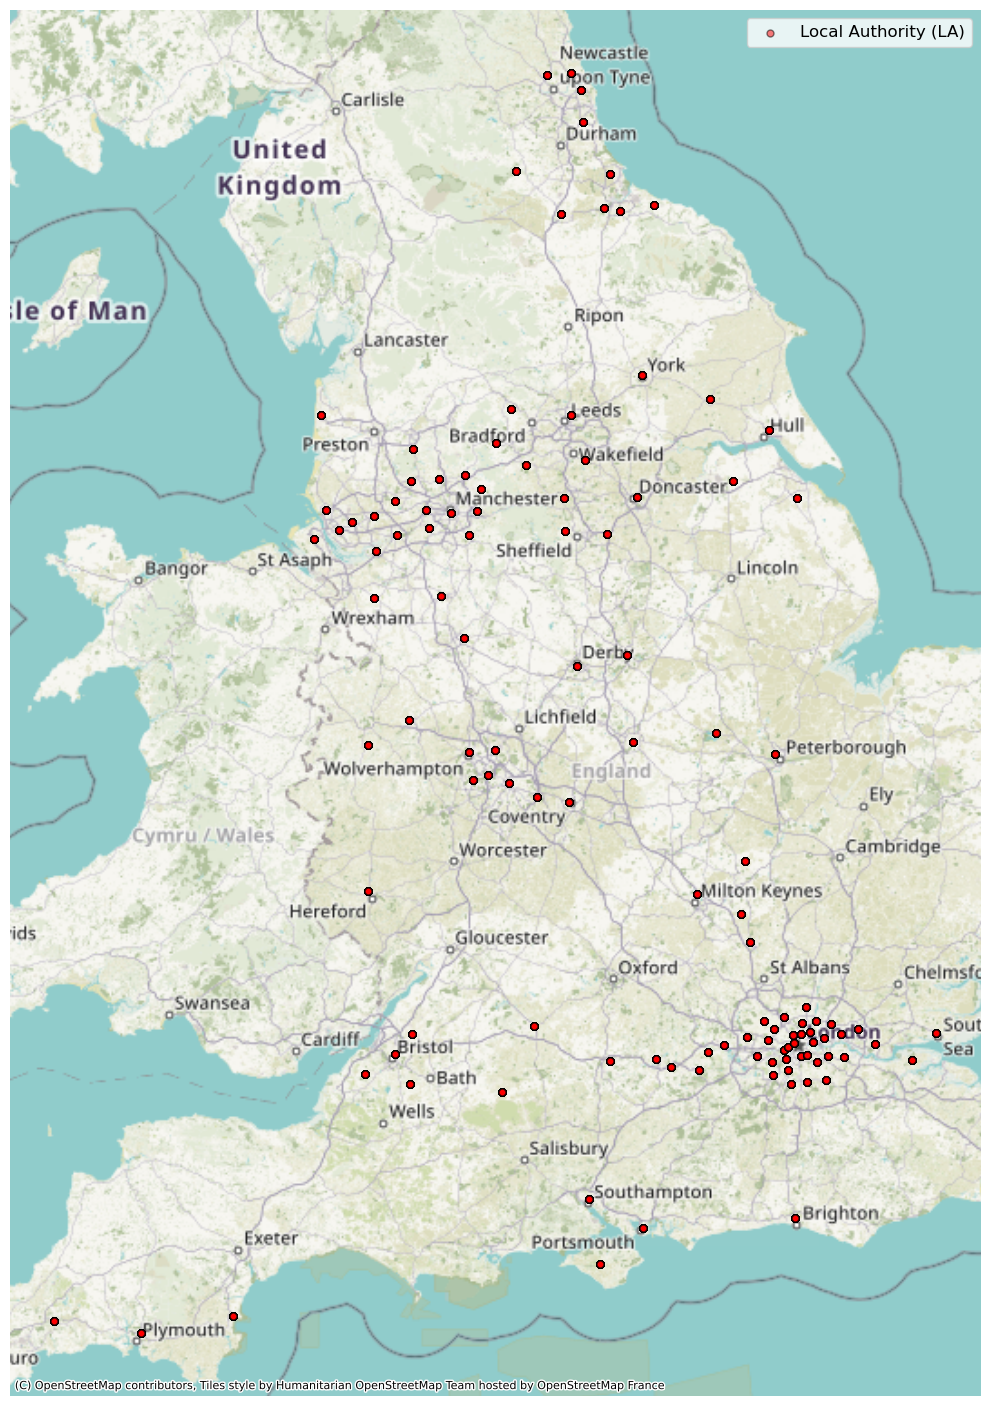
\includegraphics[keepaspectratio]{index_files/figure-pdf/fig-geo-output-1.png}}

}

\caption{\label{fig-geo}Geographic location of LAs on a map of the UK}

\end{figure}%

We can see a few things that need to be considered, as the dataset is:

\begin{itemize}
\tightlist
\item
  Restricted to England LAs
\item
  Incomplete for England, excluding key areas such as Cheltenham, Exeter
  and Oxford. This could introduce sample selection bias
\item
  Heavily skewed towards the South East and London (although this may
  reflect real-world commuting patterns)
\end{itemize}

If we look take a look a random subsample of routes\ldots{}

\begin{Shaded}
\begin{Highlighting}[]
\NormalTok{unique\_routes }\OperatorTok{=}\NormalTok{ LAcommute[[}\StringTok{\textquotesingle{}area\_name\_origin\textquotesingle{}}\NormalTok{,}
                           \StringTok{\textquotesingle{}area\_name\_dest\textquotesingle{}}\NormalTok{]].drop\_duplicates()}
\NormalTok{random\_routes }\OperatorTok{=}\NormalTok{ unique\_routes.sample(n}\OperatorTok{=}\DecValTok{3}\NormalTok{, random\_state}\OperatorTok{=}\DecValTok{0}\NormalTok{)}

\NormalTok{plotting\_routes }\OperatorTok{=}\NormalTok{ LAcommute.merge(}
\NormalTok{    random\_routes,}
\NormalTok{    on}\OperatorTok{=}\NormalTok{[}\StringTok{\textquotesingle{}area\_name\_origin\textquotesingle{}}\NormalTok{, }\StringTok{\textquotesingle{}area\_name\_dest\textquotesingle{}}\NormalTok{]}
\NormalTok{)}
\NormalTok{plotting\_routes[}\StringTok{\textquotesingle{}route\textquotesingle{}}\NormalTok{] }\OperatorTok{=}\NormalTok{ plotting\_routes[}\StringTok{\textquotesingle{}area\_name\_origin\textquotesingle{}}\NormalTok{] }\OperatorTok{+} \OperatorTok{\textbackslash{}}
    \StringTok{\textquotesingle{} to \textquotesingle{}} \OperatorTok{+}\NormalTok{ plotting\_routes[}\StringTok{\textquotesingle{}area\_name\_dest\textquotesingle{}}\NormalTok{]}

\NormalTok{plt.figure(figsize}\OperatorTok{=}\NormalTok{(}\DecValTok{12}\NormalTok{, }\DecValTok{6}\NormalTok{))}
\NormalTok{sns.lineplot(data}\OperatorTok{=}\NormalTok{plotting\_routes, x}\OperatorTok{=}\StringTok{\textquotesingle{}date\textquotesingle{}}\NormalTok{, y}\OperatorTok{=}\StringTok{\textquotesingle{}journey\_score\textquotesingle{}}\NormalTok{, hue}\OperatorTok{=}\StringTok{\textquotesingle{}route\textquotesingle{}}\NormalTok{)}

\NormalTok{plt.xlabel(}\StringTok{\textquotesingle{}Date\textquotesingle{}}\NormalTok{)}
\NormalTok{plt.ylabel(}\StringTok{\textquotesingle{}Journey Score\textquotesingle{}}\NormalTok{)}
\NormalTok{plt.title(}\StringTok{\textquotesingle{}Journey Score Over Time for Selected Routes\textquotesingle{}}\NormalTok{)}
\NormalTok{plt.grid(}\VariableTok{True}\NormalTok{)}
\NormalTok{plt.legend(title}\OperatorTok{=}\StringTok{\textquotesingle{}Route\textquotesingle{}}\NormalTok{)}
\NormalTok{plt.show()}
\end{Highlighting}
\end{Shaded}

\begin{figure}[H]

\centering{

\pandocbounded{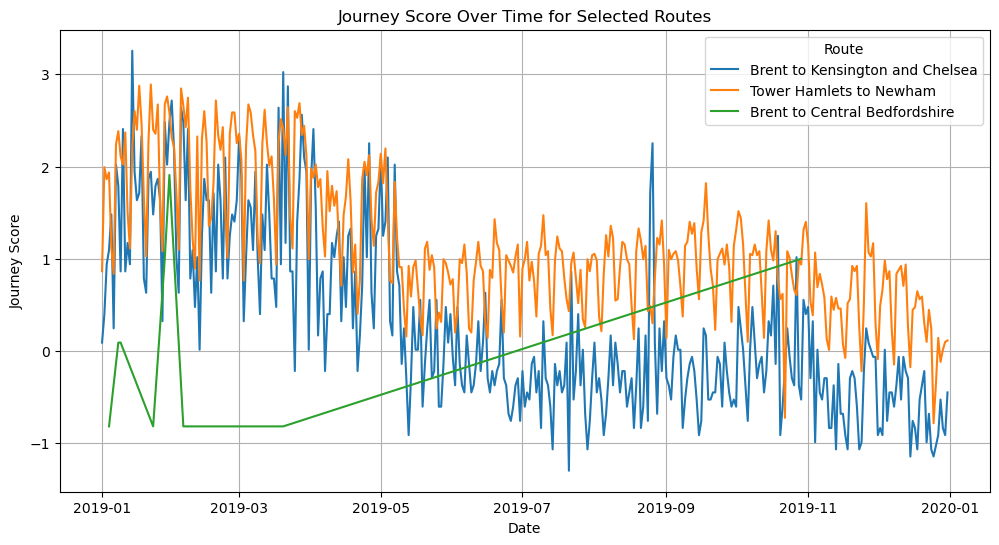
\includegraphics[keepaspectratio]{index_files/figure-pdf/fig-random_routes_score-output-1.png}}

}

\caption{\label{fig-random_routes_score}Line graph of journey scores for
random routes}

\end{figure}%

And with
\texttt{\textquotesingle{}journey\_count\_decile\textquotesingle{}}:

\begin{Shaded}
\begin{Highlighting}[]
\NormalTok{unique\_routes }\OperatorTok{=}\NormalTok{ LAcommute[[}\StringTok{\textquotesingle{}area\_name\_origin\textquotesingle{}}\NormalTok{,}
                           \StringTok{\textquotesingle{}area\_name\_dest\textquotesingle{}}\NormalTok{]].drop\_duplicates()}
\NormalTok{random\_routes }\OperatorTok{=}\NormalTok{ unique\_routes.sample(n}\OperatorTok{=}\DecValTok{3}\NormalTok{, random\_state}\OperatorTok{=}\DecValTok{0}\NormalTok{)}

\NormalTok{plotting\_routes }\OperatorTok{=}\NormalTok{ LAcommute.merge(}
\NormalTok{    random\_routes,}
\NormalTok{    on}\OperatorTok{=}\NormalTok{[}\StringTok{\textquotesingle{}area\_name\_origin\textquotesingle{}}\NormalTok{, }\StringTok{\textquotesingle{}area\_name\_dest\textquotesingle{}}\NormalTok{]}
\NormalTok{)}
\NormalTok{plotting\_routes[}\StringTok{\textquotesingle{}route\textquotesingle{}}\NormalTok{] }\OperatorTok{=}\NormalTok{ plotting\_routes[}\StringTok{\textquotesingle{}area\_name\_origin\textquotesingle{}}\NormalTok{] }\OperatorTok{+} \OperatorTok{\textbackslash{}}
    \StringTok{\textquotesingle{} to \textquotesingle{}} \OperatorTok{+}\NormalTok{ plotting\_routes[}\StringTok{\textquotesingle{}area\_name\_dest\textquotesingle{}}\NormalTok{]}

\NormalTok{plt.figure(figsize}\OperatorTok{=}\NormalTok{(}\DecValTok{12}\NormalTok{, }\DecValTok{6}\NormalTok{))}
\NormalTok{sns.lineplot(data}\OperatorTok{=}\NormalTok{plotting\_routes, x}\OperatorTok{=}\StringTok{\textquotesingle{}date\textquotesingle{}}\NormalTok{, y}\OperatorTok{=}\StringTok{\textquotesingle{}journey\_count\_decile\textquotesingle{}}\NormalTok{, hue}\OperatorTok{=}\StringTok{\textquotesingle{}route\textquotesingle{}}\NormalTok{)}

\NormalTok{plt.xlabel(}\StringTok{\textquotesingle{}Date\textquotesingle{}}\NormalTok{)}
\NormalTok{plt.ylabel(}\StringTok{\textquotesingle{}Journey Count Decile\textquotesingle{}}\NormalTok{)}
\NormalTok{plt.title(}\StringTok{\textquotesingle{}Journey Count Decile Over Time for Selected Routes\textquotesingle{}}\NormalTok{)}
\NormalTok{plt.grid(}\VariableTok{True}\NormalTok{)}
\NormalTok{plt.legend(title}\OperatorTok{=}\StringTok{\textquotesingle{}Route\textquotesingle{}}\NormalTok{, loc}\OperatorTok{=}\StringTok{\textquotesingle{}upper right\textquotesingle{}}\NormalTok{)}
\NormalTok{plt.show()}
\end{Highlighting}
\end{Shaded}

\begin{figure}[H]

\centering{

\pandocbounded{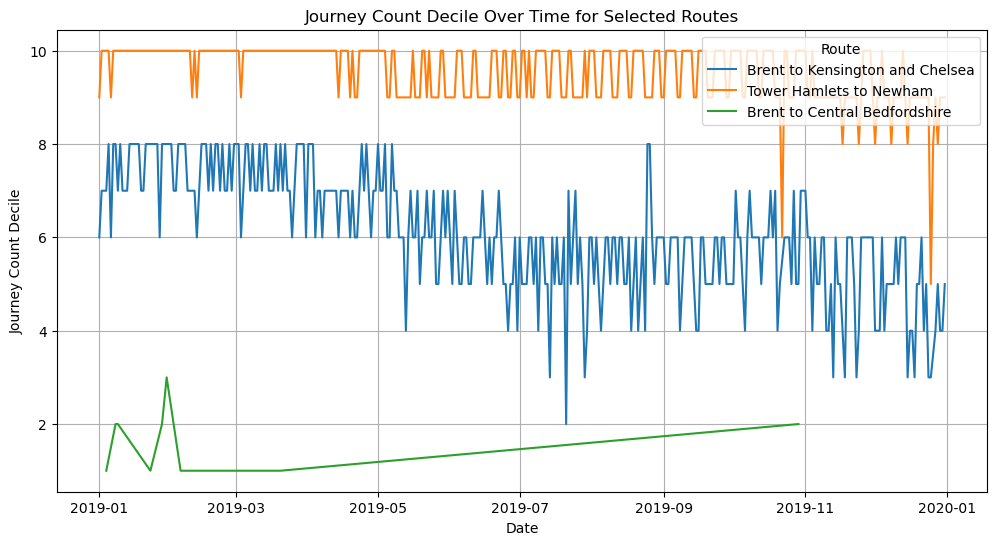
\includegraphics[keepaspectratio]{index_files/figure-pdf/fig-random_routes_deciles-output-1.png}}

}

\caption{\label{fig-random_routes_deciles}Line graph of journey count
decile for random routes}

\end{figure}%

A few important things can be deduced about the wider dataset:

\begin{itemize}
\tightlist
\item
  There is significant variation in the
  \texttt{\textquotesingle{}journey\_score,\textquotesingle{}}
  i.e.~som,e routes becoming both more and less popular over time ~ -
  There is less variation in the
  \texttt{\textquotesingle{}jouney\_count\_decile\textquotesingle{}}
  variable, which is likely a result of the aggregation process ~ - This
  will be critical for inferential design/feature selection, as the
  provided dataset suggested independent variables are all ``point in
  time'' rather than time series data
\item
  The routes are not constant over time, or there is data missing ~ ~-
  This is shown via ``Brent'' to ``Central Bedfordshire'', which does
  not show any data in December 2019
\item
  There are some irregularities, such as the ``Brent'' route flatlining,
  which could be a result of data collection/input errors
\end{itemize}

To get a bit more insight, we can look at the means:

\begin{Shaded}
\begin{Highlighting}[]
\NormalTok{means }\OperatorTok{=}\NormalTok{ LAcommute.groupby([}\StringTok{\textquotesingle{}area\_name\_origin\textquotesingle{}}\NormalTok{, }\StringTok{\textquotesingle{}area\_name\_dest\textquotesingle{}}\NormalTok{])[}\StringTok{\textquotesingle{}journey\_score\textquotesingle{}}\NormalTok{].mean()}
\NormalTok{route\_means }\OperatorTok{=} \BuiltInTok{round}\NormalTok{(means,}\DecValTok{3}\NormalTok{).reset\_index()}
\NormalTok{route\_means.columns }\OperatorTok{=}\NormalTok{ [}\StringTok{\textquotesingle{}area\_name\_origin\textquotesingle{}}\NormalTok{, }\StringTok{\textquotesingle{}area\_name\_dest\textquotesingle{}}\NormalTok{, }\StringTok{\textquotesingle{}mean\_journey\_score\textquotesingle{}}\NormalTok{]}

\NormalTok{route\_means}
\end{Highlighting}
\end{Shaded}

\begin{longtable}[]{@{}llll@{}}
\toprule\noalign{}
& area\_name\_origin & area\_name\_dest & mean\_journey\_score \\
\midrule\noalign{}
\endhead
\bottomrule\noalign{}
\endlastfoot
0 & Barking and Dagenham & Barking and Dagenham & 1.155 \\
1 & Barking and Dagenham & Brent & 0.000 \\
2 & Barking and Dagenham & Camden & 0.010 \\
3 & Barking and Dagenham & Enfield & 0.016 \\
4 & Barking and Dagenham & Greenwich & 0.030 \\
... & ... & ... & ... \\
1388 & Wolverhampton & Wolverhampton & 1.190 \\
1389 & York & East Riding of Yorkshire & 0.148 \\
1390 & York & Leeds & 0.161 \\
1391 & York & Wakefield & 0.000 \\
1392 & York & York & 1.200 \\
\end{longtable}

This shows the dataset is not standardised across routes, i.e.~not
reflecting relative popularity over time of the same route

From here on, information may be relevant to the analysis, so the file
will be saved and renamed ``LAcommute\_clean.csv.''

Geographical data will be dropped as it will be added later, where
relevant for feature additions rather than exploratory data analysis.

\begin{longtable}[]{@{}llllllllllllllllllllll@{}}
\toprule\noalign{}
& date & area\_name\_origin & area\_code\_origin & area\_name\_dest &
area\_code\_dest & journey\_score & journey\_count\_decile & distance &
population\_origin & population\_dest & ... & travel\_time\_dest &
gcse\_rate\_dest & life\_satisfaction\_dest & housing\_growth\_dest &
lat\_origin & long\_origin & lat\_dest & long\_dest & geometry\_origin &
geometry\_dest \\
\midrule\noalign{}
\endhead
\bottomrule\noalign{}
\endlastfoot
0 & 2019-01-01 & Hartlepool & E06000001 & Hartlepool & E06000001 &
1.4414 & 9 & 0.000000 & 92401 & 92401 & ... & 12.9 & 67.6 & 7.33 & 161 &
54.676140 & -1.27018 & 54.676140 & -1.27018 & POINT (-1.27018 54.67614)
& POINT (-1.27018 54.67614) \\
1 & 2019-01-01 & Hartlepool & E06000001 & County Durham & E06000047 &
-0.3129 & 3 & 37592.170378 & 92401 & 518562 & ... & 14.1 & 67.6 & 7.43 &
1343 & 54.676140 & -1.27018 & 54.685131 & -1.84050 & POINT (-1.27018
54.67614) & POINT (-1.84050 54.68513) \\
2 & 2019-01-01 & Middlesbrough & E06000002 & Middlesbrough & E06000002 &
1.0253 & 10 & 0.000000 & 142134 & 142134 & ... & 15.4 & 63.2 & 7.21 &
456 & 54.544670 & -1.21099 & 54.544670 & -1.21099 & POINT (-1.21099
54.54467) & POINT (-1.21099 54.54467) \\
3 & 2019-01-01 & Middlesbrough & E06000002 & Redcar and Cleveland &
E06000003 & 0.3086 & 7 & 13069.176565 & 142134 & 136699 & ... & 13.3 &
69.6 & 7.44 & 365 & 54.544670 & -1.21099 & 54.567520 & -1.00608 & POINT
(-1.21099 54.54467) & POINT (-1.00608 54.56752) \\
4 & 2019-01-01 & Middlesbrough & E06000002 & Stockton-on-Tees &
E06000004 & 0.3772 & 8 & 7379.212731 & 142134 & 196860 & ... & 13.2 &
69.5 & 7.40 & 616 & 54.544670 & -1.21099 & 54.556911 & -1.30664 & POINT
(-1.21099 54.54467) & POINT (-1.30664 54.55691) \\
... & ... & ... & ... & ... & ... & ... & ... & ... & ... & ... & ... &
... & ... & ... & ... & ... & ... & ... & ... & ... & ... \\
301022 & 2019-12-31 & Westminster & E09000033 & Sutton & E09000029 &
-0.6732 & 4 & 16964.439602 & 208415 & 208516 & ... & 9.0 & 82.0 & 7.36 &
313 & 51.512199 & -0.15295 & 51.357559 & -0.17227 & POINT (-0.15295
51.51220) & POINT (-0.17227 51.35756) \\
301023 & 2019-12-31 & Westminster & E09000033 & Tower Hamlets &
E09000030 & 1.3720 & 10 & 8616.142460 & 208415 & 305066 & ... & 4.4 &
72.4 & 7.13 & 3248 & 51.512199 & -0.15295 & 51.515541 & -0.03643 & POINT
(-0.15295 51.51220) & POINT (-0.03643 51.51554) \\
301024 & 2019-12-31 & Westminster & E09000033 & Waltham Forest &
E09000031 & -0.4483 & 6 & 13672.865893 & 208415 & 281015 & ... & 7.2 &
71.5 & 7.30 & 1263 & 51.512199 & -0.15295 & 51.594608 & -0.01881 & POINT
(-0.15295 51.51220) & POINT (-0.01881 51.59461) \\
301025 & 2019-12-31 & Westminster & E09000033 & Wandsworth & E09000032 &
0.1871 & 8 & 7117.584240 & 208415 & 334558 & ... & 6.2 & 74.2 & 7.34 &
1415 & 51.512199 & -0.15295 & 51.452400 & -0.20023 & POINT (-0.15295
51.51220) & POINT (-0.20023 51.45240) \\
301026 & 2019-12-31 & Westminster & E09000033 & Westminster & E09000033
& 1.6534 & 10 & 0.000000 & 208415 & 208415 & ... & 5.1 & 77.3 & 7.21 &
580 & 51.512199 & -0.15295 & 51.512199 & -0.15295 & POINT (-0.15295
51.51220) & POINT (-0.15295 51.51220) \\
\end{longtable}

\begin{Shaded}
\begin{Highlighting}[]
\NormalTok{LAcommute }\OperatorTok{=}\NormalTok{ LAcommute.drop(columns}\OperatorTok{=}\NormalTok{[}
                           \StringTok{\textquotesingle{}lat\_origin\textquotesingle{}}\NormalTok{, }\StringTok{\textquotesingle{}long\_origin\textquotesingle{}}\NormalTok{, }\StringTok{\textquotesingle{}lat\_dest\textquotesingle{}}\NormalTok{, }\StringTok{\textquotesingle{}long\_dest\textquotesingle{}}\NormalTok{, }\StringTok{\textquotesingle{}geometry\_origin\textquotesingle{}}\NormalTok{, }\StringTok{\textquotesingle{}geometry\_dest\textquotesingle{}}\NormalTok{])}

\NormalTok{LAcommute.to\_csv(}
\NormalTok{    os.path.join(base\_data\_dir, }\StringTok{"LAcommute\_clean.csv"}\NormalTok{), index}\OperatorTok{=}\VariableTok{True}
\NormalTok{)}
\end{Highlighting}
\end{Shaded}

\subsection{Appendix C: Centrality}\label{sec-centrality-appendix}

Exploring centrality using network graphs:

I will look at degree centrality for undirected networks, i.e.~who has
the most connections in terms of the number of links per node, although
there are other measures of centrality.

\begin{longtable}[]{@{}llllllllllllllllllllll@{}}
\toprule\noalign{}
& date & area\_name\_origin & area\_code\_origin & area\_name\_dest &
area\_code\_dest & journey\_score & journey\_count\_decile & distance &
population\_origin & population\_dest & ... & median\_weekly\_pay\_dest
& emp\_rate\_dest & travel\_time\_dest & gcse\_rate\_dest &
life\_satisfaction\_dest & housing\_growth\_dest & lat\_origin &
long\_origin & lat\_dest & long\_dest \\
\midrule\noalign{}
\endhead
\bottomrule\noalign{}
\endlastfoot
0 & 2019-01-02 & Hartlepool & E06000001 & Stockton-on-Tees & E06000004 &
1.5423 & 5 & 12951.008041 & 92401 & 196860 & ... & 469.4 & 74.8 & 13.2 &
69.5 & 7.40 & 616 & 54.676140 & -1.27018 & 54.556911 & -1.30664 \\
1 & 2019-01-02 & Hartlepool & E06000001 & County Durham & E06000047 &
1.5683 & 5 & 37592.170378 & 92401 & 518562 & ... & 469.4 & 71.4 & 14.1 &
67.6 & 7.43 & 1343 & 54.676140 & -1.27018 & 54.685131 & -1.84050 \\
2 & 2019-01-02 & Middlesbrough & E06000002 & Redcar and Cleveland &
E06000003 & 0.9239 & 8 & 13069.176565 & 142134 & 136699 & ... & 439.2 &
68.4 & 13.3 & 69.6 & 7.44 & 365 & 54.544670 & -1.21099 & 54.567520 &
-1.00608 \\
3 & 2019-01-02 & Middlesbrough & E06000002 & Stockton-on-Tees &
E06000004 & 1.8569 & 9 & 7379.212731 & 142134 & 196860 & ... & 469.4 &
74.8 & 13.2 & 69.5 & 7.40 & 616 & 54.544670 & -1.21099 & 54.556911 &
-1.30664 \\
4 & 2019-01-02 & Middlesbrough & E06000002 & County Durham & E06000047 &
-1.0400 & 1 & 43441.543055 & 142134 & 518562 & ... & 469.4 & 71.4 & 14.1
& 67.6 & 7.43 & 1343 & 54.544670 & -1.21099 & 54.685131 & -1.84050 \\
... & ... & ... & ... & ... & ... & ... & ... & ... & ... & ... & ... &
... & ... & ... & ... & ... & ... & ... & ... & ... & ... \\
188229 & 2019-12-31 & Westminster & E09000033 & Southwark & E09000028 &
1.0626 & 10 & 7319.207505 & 208415 & 312591 & ... & 631.9 & 79.4 & 6.1 &
71.0 & 7.17 & 1096 & 51.512199 & -0.15295 & 51.465919 & -0.07306 \\
188230 & 2019-12-31 & Westminster & E09000033 & Sutton & E09000029 &
-0.6732 & 4 & 16964.439602 & 208415 & 208516 & ... & 565.8 & 77.4 & 9.0
& 82.0 & 7.36 & 313 & 51.512199 & -0.15295 & 51.357559 & -0.17227 \\
188231 & 2019-12-31 & Westminster & E09000033 & Tower Hamlets &
E09000030 & 1.3720 & 10 & 8616.142460 & 208415 & 305066 & ... & 680.3 &
74.4 & 4.4 & 72.4 & 7.13 & 3248 & 51.512199 & -0.15295 & 51.515541 &
-0.03643 \\
188232 & 2019-12-31 & Westminster & E09000033 & Waltham Forest &
E09000031 & -0.4483 & 6 & 13672.865893 & 208415 & 281015 & ... & 624.7 &
71.5 & 7.2 & 71.5 & 7.30 & 1263 & 51.512199 & -0.15295 & 51.594608 &
-0.01881 \\
188233 & 2019-12-31 & Westminster & E09000033 & Wandsworth & E09000032 &
0.1871 & 8 & 7117.584240 & 208415 & 334558 & ... & 746.7 & 84.9 & 6.2 &
74.2 & 7.34 & 1415 & 51.512199 & -0.15295 & 51.452400 & -0.20023 \\
\end{longtable}

\begin{Shaded}
\begin{Highlighting}[]
\NormalTok{G }\OperatorTok{=}\NormalTok{ nx.Graph()}
\ControlFlowTok{for}\NormalTok{ \_, row }\KeywordTok{in}\NormalTok{ commute\_centr.iterrows():}
\NormalTok{    G.add\_edge(row[}\StringTok{\textquotesingle{}area\_name\_origin\textquotesingle{}}\NormalTok{], row[}\StringTok{\textquotesingle{}area\_name\_dest\textquotesingle{}}\NormalTok{])}
\end{Highlighting}
\end{Shaded}

\begin{Shaded}
\begin{Highlighting}[]
\NormalTok{plt.figure(figsize}\OperatorTok{=}\NormalTok{(}\DecValTok{24}\NormalTok{, }\DecValTok{24}\NormalTok{))}
\NormalTok{pos }\OperatorTok{=}\NormalTok{ nx.circular\_layout(G)}
\NormalTok{nx.draw(}
\NormalTok{    G, pos, with\_labels}\OperatorTok{=}\VariableTok{False}\NormalTok{,}
\NormalTok{    node\_size}\OperatorTok{=}\DecValTok{500}\NormalTok{, node\_color}\OperatorTok{=}\StringTok{\textquotesingle{}orange\textquotesingle{}}\NormalTok{,}
\NormalTok{    edge\_color}\OperatorTok{=}\StringTok{\textquotesingle{}gray\textquotesingle{}}
\NormalTok{)}
\ControlFlowTok{for}\NormalTok{ node, (x, y) }\KeywordTok{in}\NormalTok{ pos.items():}
\NormalTok{    angle }\OperatorTok{=}\NormalTok{ np.arctan2(y, x)}
\NormalTok{    rotation }\OperatorTok{=}\NormalTok{ np.degrees(angle)}
    \ControlFlowTok{if}\NormalTok{ x }\OperatorTok{\textless{}} \DecValTok{0}\NormalTok{:}
\NormalTok{        rotation }\OperatorTok{+=} \DecValTok{180}
\NormalTok{    plt.text(}
\NormalTok{        x, y, node,}
\NormalTok{        fontsize}\OperatorTok{=}\DecValTok{13}\NormalTok{, color}\OperatorTok{=}\StringTok{\textquotesingle{}black\textquotesingle{}}\NormalTok{,}
\NormalTok{        ha}\OperatorTok{=}\StringTok{\textquotesingle{}center\textquotesingle{}}\NormalTok{, va}\OperatorTok{=}\StringTok{\textquotesingle{}center\textquotesingle{}}\NormalTok{,}
\NormalTok{        rotation}\OperatorTok{=}\NormalTok{rotation, rotation\_mode}\OperatorTok{=}\StringTok{\textquotesingle{}anchor\textquotesingle{}}
\NormalTok{    )}
\NormalTok{plt.title(}\StringTok{\textquotesingle{}Network Graph of Commuting Routes\textquotesingle{}}\NormalTok{, fontsize}\OperatorTok{=}\DecValTok{28}\NormalTok{)}
\NormalTok{plt.show()}
\end{Highlighting}
\end{Shaded}

\begin{figure}[H]

\centering{

\pandocbounded{\includegraphics[keepaspectratio]{index_files/figure-pdf/fig-centr-output-1.png}}

}

\caption{\label{fig-centr}Network Graph of Commuting Routes}

\end{figure}%

\subsection{Appendix D: Data Diagnostics}\label{sec-data-diagnostics}

\begin{Shaded}
\begin{Highlighting}[]
\NormalTok{commute\_trans}
\end{Highlighting}
\end{Shaded}

\begin{longtable}[]{@{}llllllllllllllll@{}}
\toprule\noalign{}
& pairs & journey\_score & journey\_count\_decile & distance &
\textbar\_population\_diff\_\textbar{} &
\textbar\_value\_added\_hourly\_diff\_\textbar{} &
\textbar\_median\_weekly\_pay\_diff\_\textbar{} &
\textbar\_emp\_rate\_diff\_\textbar{} &
\textbar\_travel\_time\_diff\_\textbar{} &
\textbar\_gcse\_rate\_diff\_\textbar{} &
\textbar\_life\_satisfaction\_diff\_\textbar{} &
\textbar\_housing\_growth\_diff\_\textbar{} &
\textbar\_avg\_monthly\_rent\_diff\_\textbar{} &
\textbar\_centrality\_diff\_\textbar{} & route\_midpoint\_(geo) \\
\midrule\noalign{}
\endhead
\bottomrule\noalign{}
\endlastfoot
0 & Barking and Dagenham - Barnet & -0.010609 & 1.363636 & 25056.274464
& 171762 & 0.09 & 51.4 & 8.3 & 0.9 & 13.4 & 0.05 & 1202 & 150.0 &
0.017241 & POINT (-0.04437 51.57832) \\
1 & Barking and Dagenham - Brent & -0.397323 & 1.291667 & 27881.522854 &
128596 & 0.07 & 29.6 & 3.1 & 0.9 & 3.5 & 0.10 & 1356 & 252.0 & 0.068966
& POINT (-0.07310 51.55498) \\
2 & Barking and Dagenham - Camden & 0.112844 & 2.959443 & 20345.000863 &
1692 & 14.43 & 170.7 & 2.3 & 2.7 & 4.3 & 0.57 & 539 & 858.0 & 0.146552 &
POINT (-0.01671 51.54431) \\
3 & Barking and Dagenham - Enfield & -0.004368 & 2.500977 & 19482.245346
& 116323 & 5.36 & 15.6 & 2.5 & 0.1 & 0.7 & 0.49 & 251 & 50.0 & 0.000000
& POINT (0.02400 51.59722) \\
4 & Barking and Dagenham - Greenwich & 0.114385 & 2.973163 & 9642.046411
& 69377 & 1.56 & 95.4 & 8.3 & 0.0 & 0.8 & 0.13 & 6 & 150.0 & 0.051724 &
POINT (0.08979 51.50474) \\
... & ... & ... & ... & ... & ... & ... & ... & ... & ... & ... & ... &
... & ... & ... & ... \\
672 & West Berkshire - Wokingham & 0.163863 & 2.844894 & 29259.923429 &
10906 & 4.18 & 64.6 & 5.8 & 1.6 & 5.6 & 0.01 & 512 & 175.0 & 0.008621 &
POINT (-1.08649 51.43427) \\
673 & Westminster - Wiltshire & 0.075996 & 1.931034 & 126401.984988 &
294570 & 21.88 & 290.4 & 10.8 & 9.5 & 4.9 & 0.29 & 2266 & 1633.0 &
0.344828 & POINT (-1.03978 51.42052) \\
674 & Westminster - Windsor and Maidenhead & 0.026557 & 2.449654 &
37615.785116 & 54522 & 0.44 & 164.8 & 11.9 & 4.6 & 0.8 & 0.29 & 270 &
1183.0 & 0.318966 & POINT (-0.41418 51.49627) \\
675 & Westminster - Wokingham & -0.168467 & 1.416667 & 51144.513300 &
36626 & 4.76 & 113.0 & 10.0 & 6.8 & 3.1 & 0.12 & 549 & 1283.0 & 0.344828
& POINT (-0.52615 51.46758) \\
676 & Windsor and Maidenhead - Wokingham & 0.161748 & 2.881737 &
14209.316238 & 17896 & 5.20 & 51.8 & 1.9 & 2.2 & 2.3 & 0.17 & 819 &
100.0 & 0.025862 & POINT (-0.78738 51.45165) \\
\end{longtable}

To assess potential concerns in the data that might require
transformations, we can use histogram visualisations, scatter plots and
statistical tests:

\begin{Shaded}
\begin{Highlighting}[]
\NormalTok{numeric\_cols }\OperatorTok{=}\NormalTok{ commute\_trans.select\_dtypes(}
\NormalTok{    include}\OperatorTok{=}\NormalTok{[}\StringTok{\textquotesingle{}float64\textquotesingle{}}\NormalTok{, }\StringTok{\textquotesingle{}int64\textquotesingle{}}\NormalTok{]).columns}
\NormalTok{n\_cols }\OperatorTok{=} \DecValTok{3}
\NormalTok{n\_rows }\OperatorTok{=}\NormalTok{ (}\BuiltInTok{len}\NormalTok{(numeric\_cols) }\OperatorTok{+}\NormalTok{ n\_cols }\OperatorTok{{-}} \DecValTok{1}\NormalTok{) }\OperatorTok{//}\NormalTok{ n\_cols}

\NormalTok{fig, axes }\OperatorTok{=}\NormalTok{ plt.subplots(n\_rows, n\_cols, figsize}\OperatorTok{=}\NormalTok{(}\DecValTok{15}\NormalTok{, n\_rows }\OperatorTok{*} \DecValTok{5}\NormalTok{))}
\NormalTok{axes }\OperatorTok{=}\NormalTok{ axes.flatten()}

\NormalTok{palette }\OperatorTok{=}\NormalTok{ [}\StringTok{\textquotesingle{}\#69b3a2\textquotesingle{}}\NormalTok{]}
\NormalTok{sns.set\_theme(style}\OperatorTok{=}\StringTok{\textquotesingle{}darkgrid\textquotesingle{}}\NormalTok{)}

\ControlFlowTok{for}\NormalTok{ i, col }\KeywordTok{in} \BuiltInTok{enumerate}\NormalTok{(numeric\_cols):}
\NormalTok{    sns.histplot(commute\_trans[col], kde}\OperatorTok{=}\VariableTok{True}\NormalTok{,}
\NormalTok{                 color}\OperatorTok{=}\NormalTok{palette[}\DecValTok{0}\NormalTok{], bins}\OperatorTok{=}\DecValTok{30}\NormalTok{, ax}\OperatorTok{=}\NormalTok{axes[i])}
\NormalTok{    axes[i].set\_title(}\SpecialStringTok{f\textquotesingle{}Distribution of }\SpecialCharTok{\{}\NormalTok{col}\SpecialCharTok{\}}\SpecialStringTok{\textquotesingle{}}\NormalTok{)}
\NormalTok{    axes[i].set\_xlabel(col)}
\NormalTok{    axes[i].set\_ylabel(}\StringTok{\textquotesingle{}Frequency\textquotesingle{}}\NormalTok{)}

\ControlFlowTok{for}\NormalTok{ j }\KeywordTok{in} \BuiltInTok{range}\NormalTok{(}\BuiltInTok{len}\NormalTok{(numeric\_cols), }\BuiltInTok{len}\NormalTok{(axes)):}
\NormalTok{    fig.delaxes(axes[j])}

\NormalTok{plt.tight\_layout()}
\NormalTok{plt.show()}
\end{Highlighting}
\end{Shaded}

\begin{figure}[H]

\centering{

\pandocbounded{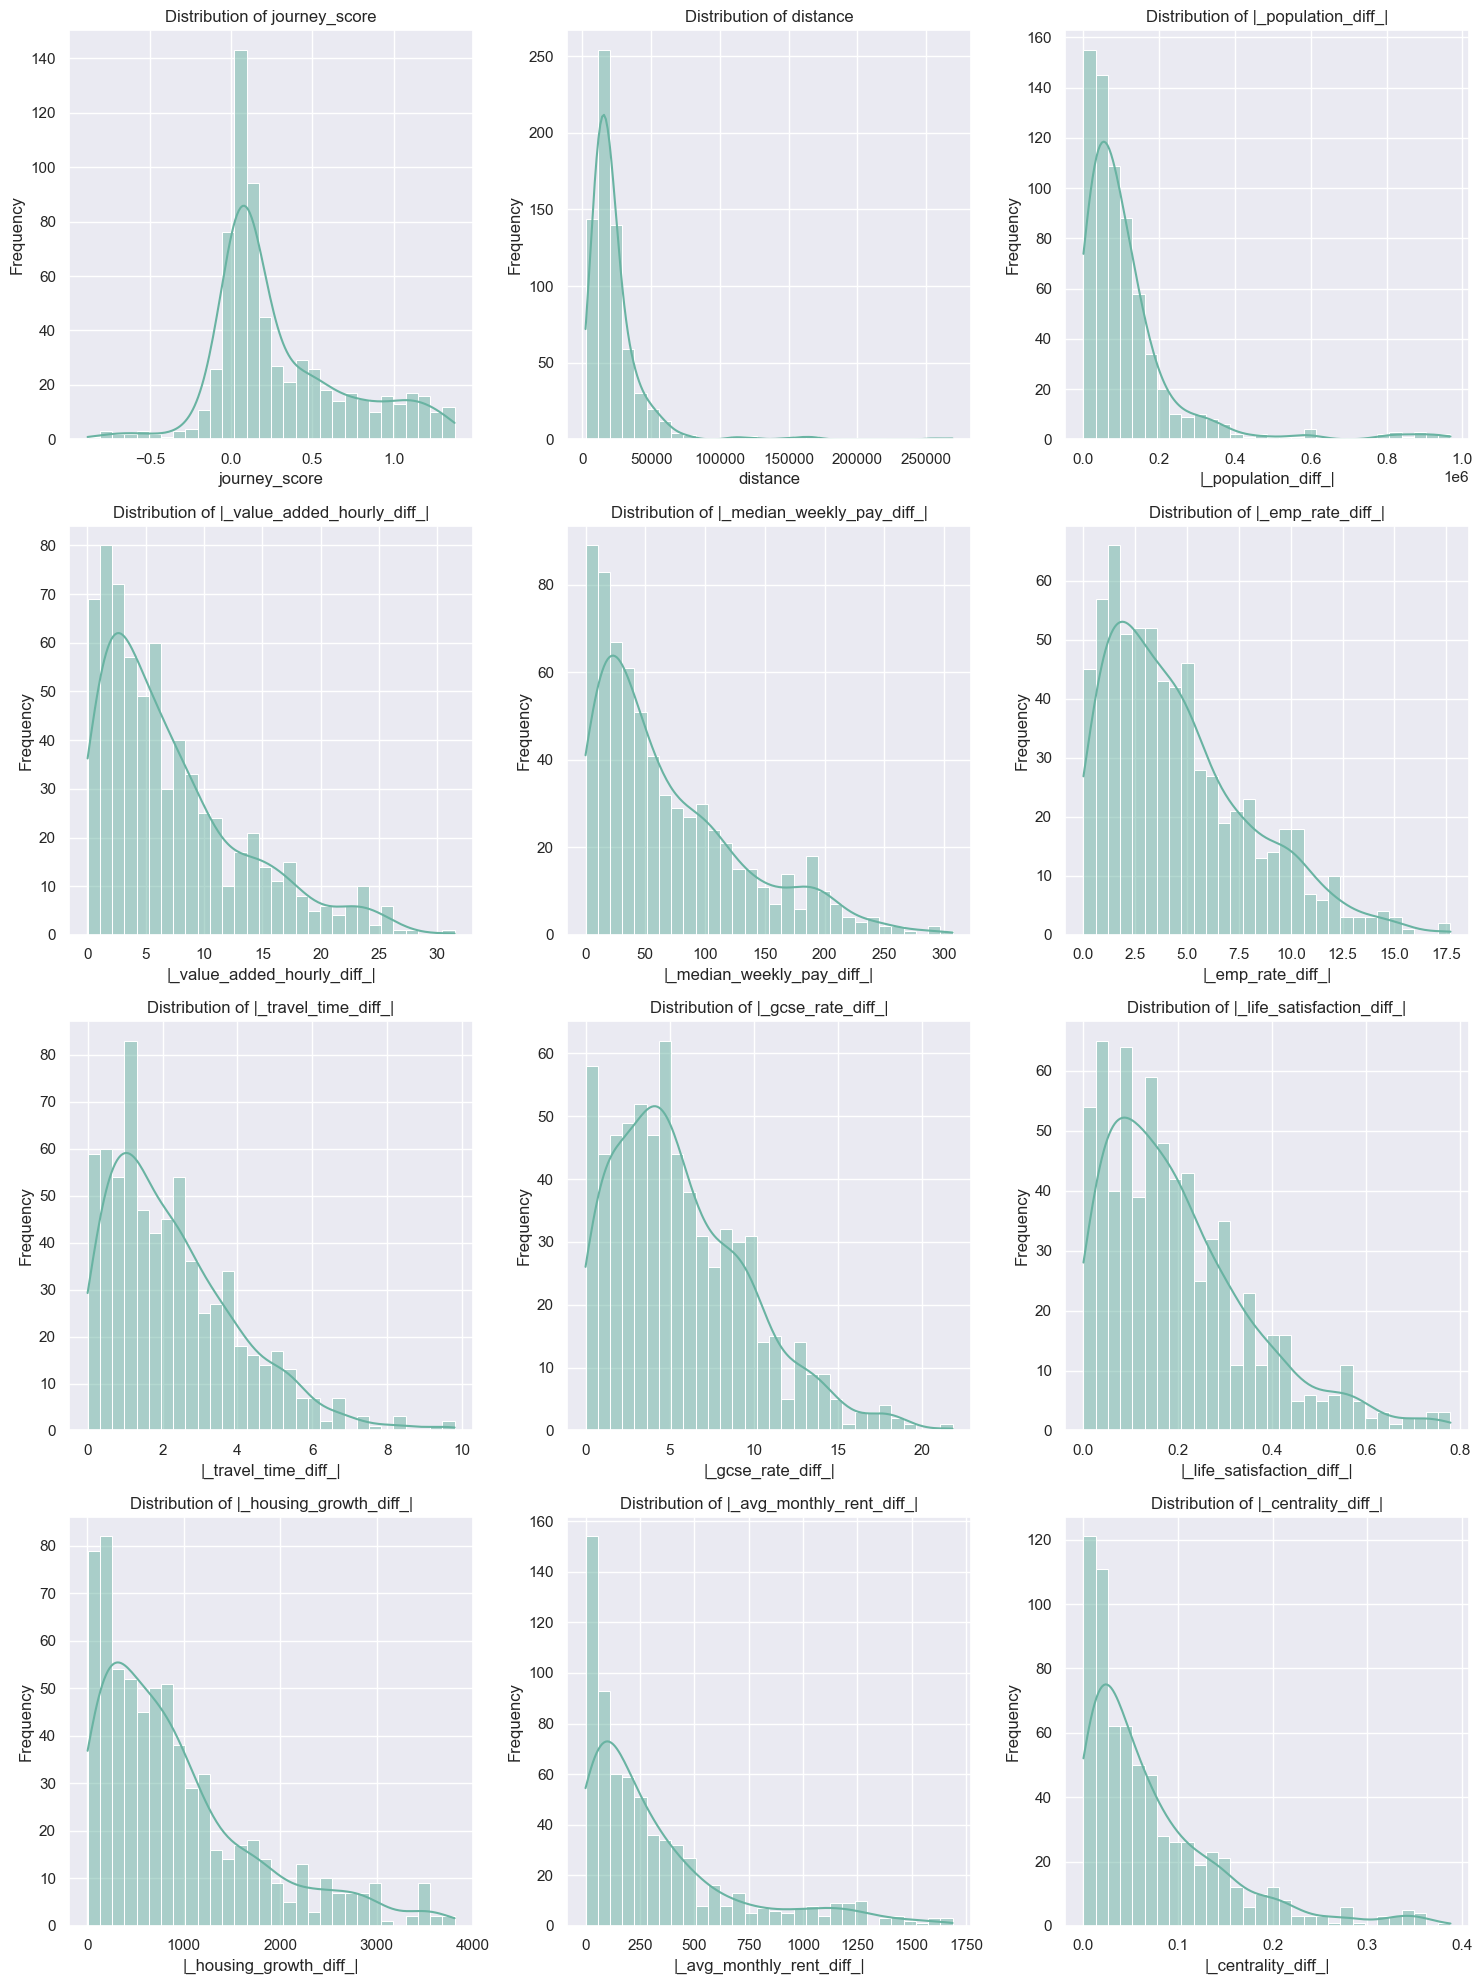
\includegraphics[keepaspectratio]{index_files/figure-pdf/fig-histogram-output-1.png}}

}

\caption{\label{fig-histogram}Histogram of distribution of commute data}

\end{figure}%

Almost all variables are rightly skewed which could be a concern for
OLS, as it violates assumptions of normality.

\begin{Shaded}
\begin{Highlighting}[]
\NormalTok{fig, axes }\OperatorTok{=}\NormalTok{ plt.subplots(n\_rows, n\_cols, figsize}\OperatorTok{=}\NormalTok{(}\DecValTok{15}\NormalTok{, n\_rows }\OperatorTok{*} \DecValTok{5}\NormalTok{))}
\NormalTok{axes }\OperatorTok{=}\NormalTok{ axes.flatten()}

\NormalTok{palette }\OperatorTok{=}\NormalTok{ [}\StringTok{\textquotesingle{}\#ffb347\textquotesingle{}}\NormalTok{]}
\NormalTok{sns.set\_theme(style}\OperatorTok{=}\StringTok{\textquotesingle{}darkgrid\textquotesingle{}}\NormalTok{)}

\ControlFlowTok{for}\NormalTok{ i, col }\KeywordTok{in} \BuiltInTok{enumerate}\NormalTok{(numeric\_cols):}
\NormalTok{    sns.boxplot(y}\OperatorTok{=}\NormalTok{commute\_trans[col], color}\OperatorTok{=}\NormalTok{palette[}\DecValTok{0}\NormalTok{], ax}\OperatorTok{=}\NormalTok{axes[i])}
\NormalTok{    axes[i].set\_title(}\SpecialStringTok{f\textquotesingle{}Box Plot of }\SpecialCharTok{\{}\NormalTok{col}\SpecialCharTok{\}}\SpecialStringTok{\textquotesingle{}}\NormalTok{)}
\NormalTok{    axes[i].set\_xlabel(}\StringTok{\textquotesingle{}\textquotesingle{}}\NormalTok{)}
\NormalTok{    axes[i].set\_ylabel(col)}

\ControlFlowTok{for}\NormalTok{ j }\KeywordTok{in} \BuiltInTok{range}\NormalTok{(}\BuiltInTok{len}\NormalTok{(numeric\_cols), }\BuiltInTok{len}\NormalTok{(axes)):}
\NormalTok{    fig.delaxes(axes[j])}

\NormalTok{plt.tight\_layout()}
\NormalTok{plt.show()}
\end{Highlighting}
\end{Shaded}

\begin{figure}[H]

\centering{

\pandocbounded{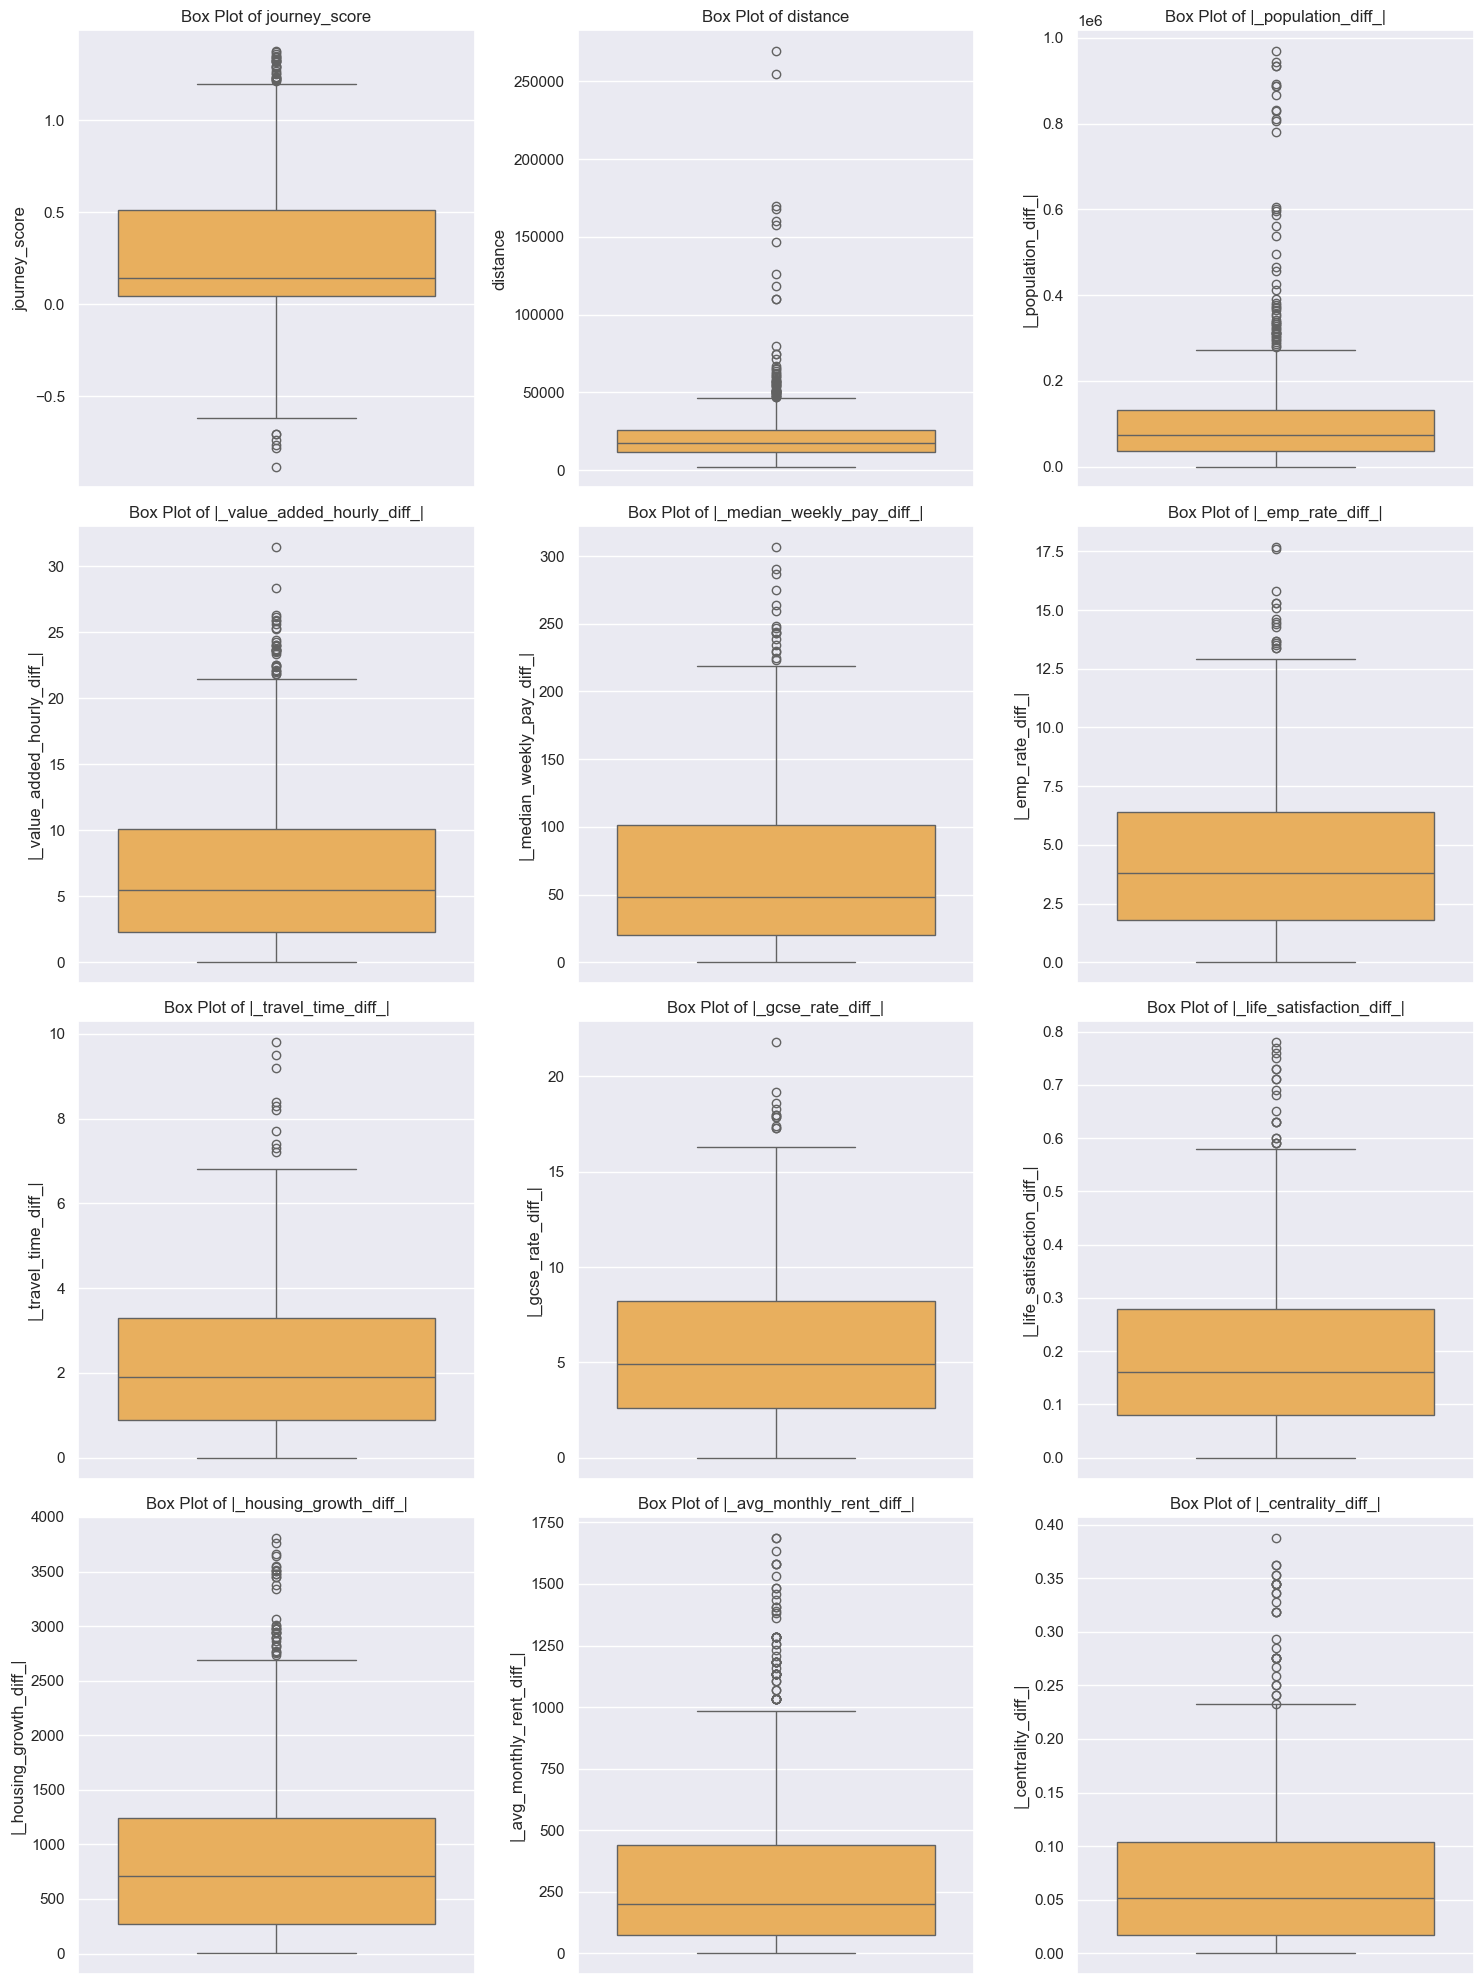
\includegraphics[keepaspectratio]{index_files/figure-pdf/fig-boxplot-output-1.png}}

}

\caption{\label{fig-boxplot}Box plot of distribution of commute data}

\end{figure}%

In addition we can look at the relationship between
\texttt{\textquotesingle{}journey\_score\textquotesingle{}} and the
other variables to assess linearity. This is important for OLS, as it
assumes a linear relationship between the dependent and independent
variables:

\begin{Shaded}
\begin{Highlighting}[]
\NormalTok{y\_sp }\OperatorTok{=} \StringTok{\textquotesingle{}journey\_score\textquotesingle{}}
\NormalTok{X\_sp }\OperatorTok{=}\NormalTok{ [col }\ControlFlowTok{for}\NormalTok{ col }\KeywordTok{in}\NormalTok{ numeric\_cols }\ControlFlowTok{if}\NormalTok{ col }\OperatorTok{!=}\NormalTok{ y\_sp]}

\NormalTok{fig, axes }\OperatorTok{=}\NormalTok{ plt.subplots(n\_rows, n\_cols, figsize}\OperatorTok{=}\NormalTok{(}\DecValTok{15}\NormalTok{, n\_rows }\OperatorTok{*} \DecValTok{5}\NormalTok{))}
\NormalTok{axes }\OperatorTok{=}\NormalTok{ axes.flatten()}

\NormalTok{palette }\OperatorTok{=}\NormalTok{ [}\StringTok{\textquotesingle{}\#ff6961\textquotesingle{}}\NormalTok{]}
\NormalTok{sns.set\_theme(style}\OperatorTok{=}\StringTok{\textquotesingle{}darkgrid\textquotesingle{}}\NormalTok{)}

\ControlFlowTok{for}\NormalTok{ i, col }\KeywordTok{in} \BuiltInTok{enumerate}\NormalTok{(X\_sp):}
\NormalTok{    sns.scatterplot(}
\NormalTok{        x}\OperatorTok{=}\NormalTok{commute\_trans[col], y}\OperatorTok{=}\NormalTok{commute\_trans[y\_sp], color}\OperatorTok{=}\NormalTok{palette[}\DecValTok{0}\NormalTok{], ax}\OperatorTok{=}\NormalTok{axes[i])}
\NormalTok{    axes[i].set\_title(}\SpecialStringTok{f\textquotesingle{}}\SpecialCharTok{\{}\NormalTok{col}\SpecialCharTok{\}}\SpecialStringTok{ vs }\SpecialCharTok{\{}\NormalTok{y\_sp}\SpecialCharTok{\}}\SpecialStringTok{\textquotesingle{}}\NormalTok{)}
\NormalTok{    axes[i].set\_xlabel(col)}
\NormalTok{    axes[i].set\_ylabel(y\_sp)}

\ControlFlowTok{for}\NormalTok{ j }\KeywordTok{in} \BuiltInTok{range}\NormalTok{(}\BuiltInTok{len}\NormalTok{(X\_sp), }\BuiltInTok{len}\NormalTok{(axes)):}
\NormalTok{    fig.delaxes(axes[j])}

\NormalTok{plt.tight\_layout()}
\NormalTok{plt.show()}
\end{Highlighting}
\end{Shaded}

\begin{figure}[H]

\centering{

\pandocbounded{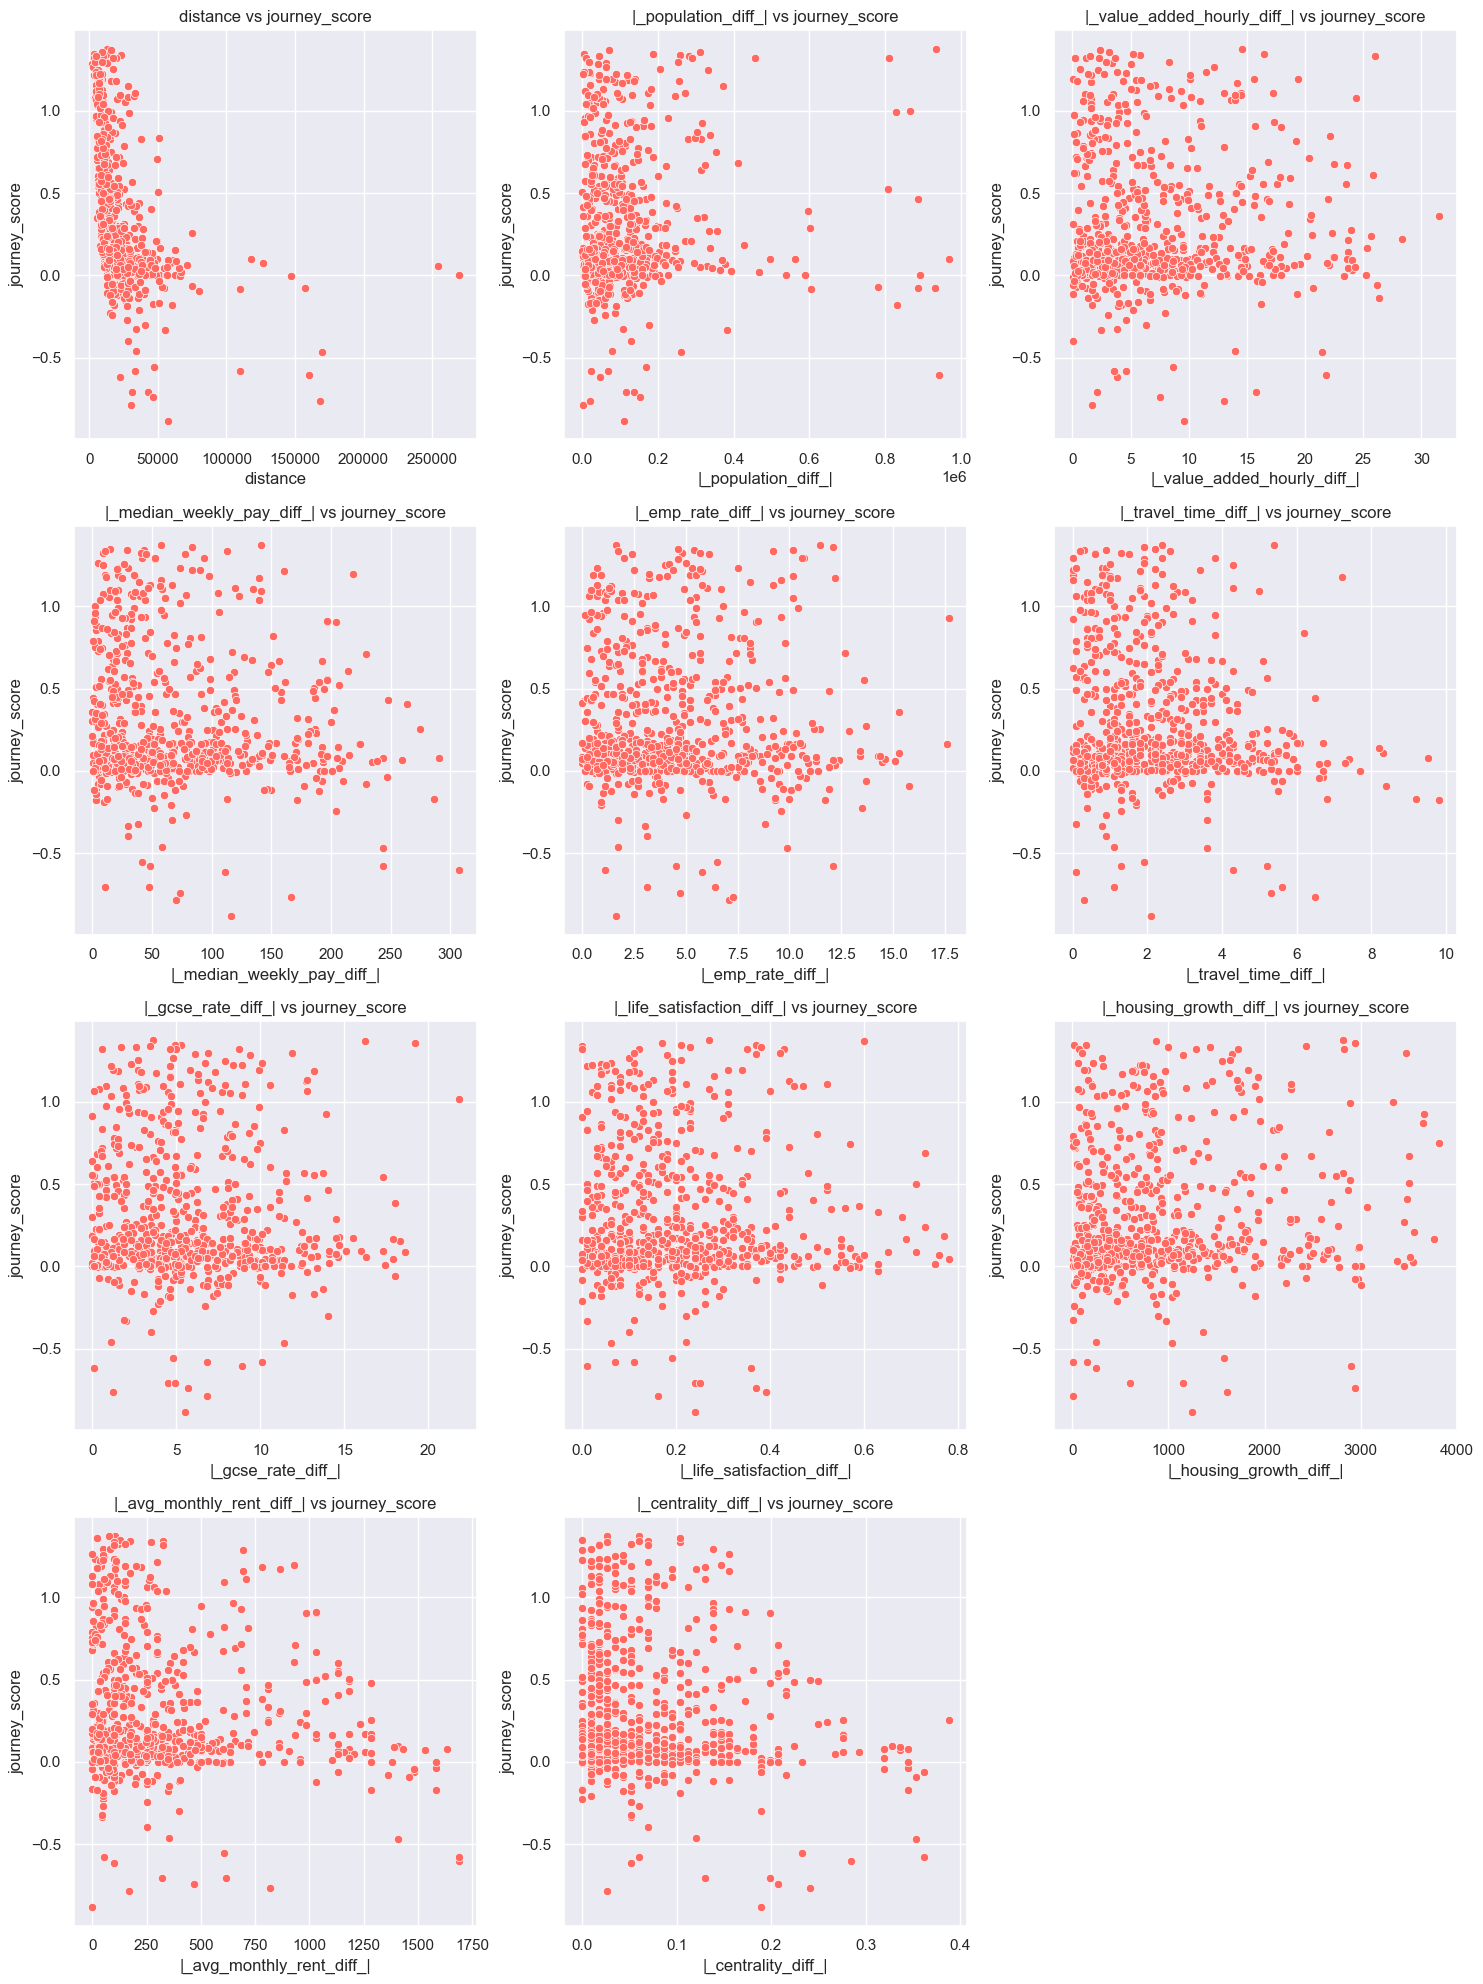
\includegraphics[keepaspectratio]{index_files/figure-pdf/fig-scatterplot-output-1.png}}

}

\caption{\label{fig-scatterplot}Scatterplot of distribution of commute
data}

\end{figure}%

\ldots{} the concerns around non-linearity are confirmed by the scatter
plot all plots show show variance of
\texttt{\textquotesingle{}journey\_score\textquotesingle{}} increasing
with X. This therefore violates a key OLS assumption.





\end{document}
